\documentclass{article}
\usepackage[utf8]{inputenc}
\usepackage{amsmath}
\usepackage{amssymb}
\usepackage{graphicx}
\usepackage{hyperref}
\usepackage{listings}
\usepackage{xcolor}
\usepackage{tikz}
\usepackage{float}
\usepackage{booktabs}
\usepackage{geometry}
\usepackage{fancyhdr}

% Define JSON language for listings
\lstdefinelanguage{JSON}{
    keywords={true,false,null},
    sensitive=true,
    comment=[l]{//},
    morecomment=[s]{/*}{*/},
    morestring=[b]",
    morestring=[d]'
}

% Set page geometry
\geometry{a4paper, margin=1in}

% Configure fancy headers
\pagestyle{fancy}
\fancyhf{}
\fancyhead[L]{Orthogonal Vectors Generator}
\fancyhead[R]{Generalized Implementation}
\fancyfoot[C]{\thepage}
\renewcommand{\headrulewidth}{0.4pt}
\renewcommand{\footrulewidth}{0.4pt}

% Define colors for code listings
\definecolor{codegreen}{rgb}{0,0.6,0}
\definecolor{codegray}{rgb}{0.5,0.5,0.5}
\definecolor{codepurple}{rgb}{0.58,0,0.82}
\definecolor{backcolour}{rgb}{0.95,0.95,0.92}

% Define code listing style
\lstdefinestyle{mystyle}{
    backgroundcolor=\color{backcolour},   
    commentstyle=\color{codegreen},
    keywordstyle=\color{magenta},
    numberstyle=\tiny\color{codegray},
    stringstyle=\color{codepurple},
    basicstyle=\ttfamily\footnotesize,
    breakatwhitespace=false,         
    breaklines=true,                 
    captionpos=b,                    
    keepspaces=true,                 
    numbers=left,                    
    numbersep=5pt,                  
    showspaces=false,                
    showstringspaces=false,
    showtabs=false,                  
    tabsize=2
}

% Set the code listing style
\lstset{style=mystyle}

% Set the graphics path
\graphicspath{{figures/}}

% Document information
\title{Generalized Orthogonal Vectors\\Generator and Visualizer}
\author{Technical Documentation}
\date{\today}

\begin{document}

\maketitle

\begin{abstract}
This document provides a comprehensive guide to the generalized implementation of the Orthogonal Vectors Generator and Visualizer. The implementation offers a modular and configurable approach to creating and visualizing three orthogonal vectors from a given origin point. This document covers the mathematical formulation, implementation details, API reference, usage examples, and visualization techniques.
\end{abstract}

\tableofcontents
\newpage

% Include the various sections from separate files
\section{Introduction}

In three-dimensional space, orthogonal vectors are perpendicular to each other, meaning their dot product equals zero. This document describes a generalized implementation for generating and visualizing three orthogonal vectors from a given origin point.

\subsection{Project Overview}

The Generalized Orthogonal Vectors Generator and Visualizer is a Python package that provides a modular and configurable approach to vector generation and visualization. It is designed to be flexible, extensible, and easy to use, both as a command-line tool and as a Python package.

\subsection{Key Features}

The generalized implementation offers the following key features:

\begin{itemize}
    \item \textbf{Modular Architecture}: The implementation is divided into separate modules for vector calculations, visualization, and configuration management.
    
    \item \textbf{Configurability}: All aspects of vector generation and visualization can be configured through a unified configuration system.
    
    \item \textbf{Command-line Interface}: A comprehensive command-line interface allows for easy use without writing Python code.
    
    \item \textbf{Configuration File Support}: Configurations can be saved to and loaded from JSON files.
    
    \item \textbf{Multiple Visualization Options}: Both 3D visualization and various 2D projections are supported.
    
    \item \textbf{Plot Saving}: Plots can be saved to files instead of being displayed interactively.
    
    \item \textbf{Python Package}: The implementation can be used as a Python package, allowing for integration into other projects.
\end{itemize}

\subsection{Package Structure}

The package is organized into the following modules:

\begin{itemize}
    \item \texttt{vector\_utils.py}: Contains functions for vector calculations, including the creation of orthogonal vectors and checking their orthogonality.
    
    \item \texttt{visualization.py}: Provides functions for visualizing vectors in 3D and 2D projections.
    
    \item \texttt{config.py}: Implements a configuration management system with the \texttt{VectorConfig} class.
    
    \item \texttt{main.py}: Provides a command-line interface for the package.
    
    \item \texttt{example.py}: Contains example scripts demonstrating different use cases.
    
    \item \texttt{\_\_init\_\_.py}: Package initialization and exports.
\end{itemize}

\subsection{Document Structure}

This document is organized as follows:

\begin{itemize}
    \item \textbf{Mathematical Formulation}: Explains the mathematical basis for generating orthogonal vectors.
    
    \item \textbf{Implementation}: Describes the implementation details of the package.
    
    \item \textbf{API Reference}: Provides a reference for the package's API.
    
    \item \textbf{Usage Examples}: Shows examples of how to use the package.
    
    \item \textbf{Visualization}: Explains the visualization techniques used.
    
    \item \textbf{Configuration}: Describes the configuration management system.
    
    \item \textbf{Command-line Interface}: Documents the command-line interface.
    
    \item \textbf{Example Results}: Shows example results for different configurations.
    
    \item \textbf{Conclusion}: Summarizes the document and discusses potential future work.
    
    \item \textbf{Appendix}: Contains additional information, including complete code listings.
\end{itemize}

\newpage
\section{Mathematical Formulation}

This section describes the mathematical basis for generating a single R vector orthogonal to the x=y=z line using basis vectors from a given origin point.

\subsection{Basis Vectors Formulation}

Let $\vec{R}_0$ be the origin vector in three-dimensional space. The R vector is calculated using basis vectors that are orthogonal to the (1,1,1) direction (the x=y=z line):

\begin{align}
\vec{R} = \vec{R}_0 + \vec{c}_1 + \vec{c}_2 + \vec{c}_3
\end{align}

where $\vec{c}_1$, $\vec{c}_2$, and $\vec{c}_3$ are component vectors calculated using two basis vectors:

\begin{align}
\vec{b}_1 &= [1, -1/2, -1/2] \quad \text{(First basis vector)} \\
\vec{b}_2 &= [0, -1/2, 1/2] \quad \text{(Second basis vector)}
\end{align}

These basis vectors are orthogonal to the (1,1,1) direction, which ensures that any linear combination of them will also be orthogonal to this direction.

The component vectors are calculated as:

\begin{align}
\vec{c}_1 &= d \cdot \cos(\theta) \cdot \sqrt{\frac{2}{3}} \cdot \vec{b}_1 \\
\vec{c}_2 &= d \cdot \frac{\cos(\theta)/\sqrt{3} + \sin(\theta)}{\sqrt{2}} \cdot \vec{b}_1 \\
\vec{c}_3 &= d \cdot \frac{\sin(\theta) - \cos(\theta)/\sqrt{3}}{\sqrt{2}} \cdot \vec{b}_2 \cdot \sqrt{2}
\end{align}

where:
\begin{itemize}
    \item $d$ is a distance parameter that scales the vector
    \item $\theta$ is an angle parameter that rotates the vector
\end{itemize}

The resulting vector $\vec{R}$ is guaranteed to be orthogonal to the (1,1,1) direction because it is constructed using basis vectors that are orthogonal to this direction.

\subsection{Perfect Orthogonal Circle Method}

In addition to the basis vectors formulation described above, we have implemented a more direct method for generating a perfect circle in the plane orthogonal to the x=y=z line. This method uses normalized basis vectors to ensure that all points are exactly at the specified distance from the origin and perfectly orthogonal to the (1,1,1) direction.

\subsubsection{Normalized Basis Vectors}

We start with the same basis vectors as before:

\begin{align}
\vec{b}_1 &= [1, -1/2, -1/2] \\
\vec{b}_2 &= [0, -1/2, 1/2]
\end{align}

But now we normalize them to ensure they have unit length:

\begin{align}
\hat{b}_1 &= \frac{\vec{b}_1}{\|\vec{b}_1\|} \\
\hat{b}_2 &= \frac{\vec{b}_2}{\|\vec{b}_2\|}
\end{align}

\subsubsection{Parametric Circle Equation}

We then use the parametric equation of a circle to generate points at a fixed distance $d$ from the origin $\vec{R}_0$:

\begin{align}
\vec{R}(\theta) = \vec{R}_0 + d \cdot (\cos(\theta) \cdot \hat{b}_1 + \sin(\theta) \cdot \hat{b}_2)
\end{align}

where $\theta$ is the angle parameter that varies from 0 to $2\pi$ to generate a full circle.

\subsubsection{Mathematical Properties}

This formulation has several important mathematical properties:

\paragraph{Exact Distance} Since $\hat{b}_1$ and $\hat{b}_2$ are unit vectors and are orthogonal to each other, the term $(\cos(\theta) \cdot \hat{b}_1 + \sin(\theta) \cdot \hat{b}_2)$ has a constant magnitude of 1 for all values of $\theta$. This ensures that all points are exactly at distance $d$ from the origin $\vec{R}_0$.

\paragraph{Perfect Orthogonality} Both $\hat{b}_1$ and $\hat{b}_2$ are orthogonal to the (1,1,1) direction, so any linear combination of them will also be orthogonal to this direction. This ensures that all points on the circle are perfectly orthogonal to the x=y=z line.

\paragraph{Perfect Circle} The use of $\cos(\theta)$ and $\sin(\theta)$ with orthogonal unit vectors ensures that the points form a perfect circle in the plane spanned by $\hat{b}_1$ and $\hat{b}_2$, which is orthogonal to the (1,1,1) direction.

\subsection{Mathematical Properties}

The basis vectors formulation has several important mathematical properties:

\subsubsection{Orthogonality to the x=y=z Line}

The key feature of this formulation is that it generates vectors that are orthogonal to the x=y=z line (the (1,1,1) direction). This is achieved by using basis vectors that are orthogonal to this direction:

\begin{align}
\vec{b}_1 \cdot [1,1,1] &= 1 \cdot 1 + (-1/2) \cdot 1 + (-1/2) \cdot 1 = 1 - 1/2 - 1/2 = 0 \\
\vec{b}_2 \cdot [1,1,1] &= 0 \cdot 1 + (-1/2) \cdot 1 + (1/2) \cdot 1 = 0 - 1/2 + 1/2 = 0
\end{align}

Since any linear combination of these basis vectors will also be orthogonal to the (1,1,1) direction, the resulting vector $\vec{R} - \vec{R}_0$ will be orthogonal to this direction regardless of the values of $d$, $\theta$, or $\vec{R}_0$.

\subsubsection{Invariance to Origin}

The behavior of the vector generation is predictable with respect to the origin point $\vec{R}_0$. The formula automatically adjusts for the origin position.

\subsubsection{Invariance to Rotation}

The parameter $\theta$ allows for rotation of the generated vector around the origin. This rotation parameter provides flexibility in generating different vector orientations.

\subsubsection{Scaling}

The parameter $d$ scales the vector magnitude, allowing for adjusting the size of the vector without changing its direction properties.

\subsection{Geometric Interpretation}

Geometrically, the basis vectors formulation generates vectors that lie in a plane orthogonal to the x=y=z line. This plane is spanned by the two basis vectors $\vec{b}_1 = [1, -1/2, -1/2]$ and $\vec{b}_2 = [0, -1/2, 1/2]$.

The parameter $d$ controls the scale of the vector, while $\theta$ controls the orientation within this orthogonal plane. As $\theta$ varies from 0 to $2\pi$, the vector traces a circle in this plane, always maintaining orthogonality to the x=y=z line.

\subsection{Circle and Sphere Generation}

One interesting application of this vector generation formula is the creation of circle and sphere-like patterns that are orthogonal to the x=y=z line. By keeping $d$ constant and varying $\theta$ from 0 to $2\pi$, the resulting endpoints of the $\vec{R}$ vectors form a pattern that lies on a circle in the plane orthogonal to the x=y=z line.

This behavior can be observed in the example scripts provided with the system:

\begin{itemize}
    \item \texttt{example\_circle.py} - Demonstrates the circle pattern orthogonal to the x=y=z line generated by varying $\theta$
    \item \texttt{example\_circle\_xy.py} - Creates a traditional circle in the XY plane for comparison
    \item \texttt{example\_orthogonal\_circle.py} - Provides improved visualization of the circle orthogonal to the x=y=z line
    \item \texttt{perfect\_orthogonal\_circle.py} - Implements the perfect circle generation with enhanced visualization
    \item \texttt{perfect\_circle\_distance\_range.py} - Demonstrates multiple perfect circles at different distances with enhanced visualization
\end{itemize}

The mathematical reason for this behavior is that the basis vectors formulation ensures that all generated vectors are orthogonal to the x=y=z line. When $\theta$ is varied, the vector traces a circle in the plane orthogonal to this line. This is fundamentally different from a traditional circle in the XY plane, which is not generally orthogonal to the x=y=z line.

The orthogonality to the x=y=z line is guaranteed by the use of basis vectors $\vec{b}_1 = [1, -1/2, -1/2]$ and $\vec{b}_2 = [0, -1/2, 1/2]$, which form a basis for the plane orthogonal to the (1,1,1) direction.

\subsection{Enhanced Visualization Techniques}

To better understand the spatial relationships and properties of these orthogonal vectors, we have implemented enhanced visualization techniques that provide clearer representation of the three-dimensional space:

\subsubsection{Color-coded Coordinate System}

The visualization uses a color-coded coordinate system to help with spatial orientation:

\begin{itemize}
    \item X-axis: Red
    \item Y-axis: Green
    \item Z-axis: Blue
\end{itemize}

This color coding follows standard conventions in computer graphics and makes it easier to identify the orientation of the three-dimensional space.

\subsubsection{Coordinate Labels and Tick Marks}

Integer coordinate values are displayed along each axis, color-matched to the axis color. Small tick marks are also added along each axis for better spatial reference. This helps in understanding the scale and position of the vectors in the three-dimensional space.

\subsubsection{Data-driven Scaling}

The axis limits are dynamically adjusted based on the actual data points, ensuring that all vectors are visible while minimizing unused space. This is particularly important when visualizing multiple vectors or circles with different parameters.

\subsubsection{Equal Aspect Ratio}

The 3D plots maintain an equal aspect ratio for accurate spatial representation. This ensures that the visualization does not distort the geometric properties of the vectors and circles, which is crucial for understanding their orthogonality and other mathematical properties.

These enhanced visualization techniques significantly improve the visual representation of the orthogonal vectors, making it easier to understand their spatial relationships and properties. They are particularly useful for visualizing the perfect orthogonal circles and their relationship to the x=y=z line.

\section{Implementation}

The generalized implementation of the Orthogonal Vectors Generator and Visualizer is designed to be modular, configurable, and easy to use. This section describes the implementation details of the package.

\subsection{Modular Architecture}

The package is organized into the following modules:

\begin{itemize}
    \item \texttt{vector\_utils.py}: Contains functions for vector calculations.
    \item \texttt{visualization.py}: Provides functions for visualizing vectors.
    \item \texttt{config.py}: Implements a configuration management system.
    \item \texttt{main.py}: Provides a command-line interface.
    \item \texttt{example.py}: Contains example scripts.
    \item \texttt{\_\_init\_\_.py}: Package initialization and exports.
\end{itemize}

This modular architecture allows for easy maintenance, extension, and reuse of the code.

\subsection{Vector Utilities}

The \texttt{vector\_utils.py} module provides functions for vector calculations, including:

\begin{itemize}
    \item \texttt{create\_orthogonal\_vectors}: Creates three orthogonal vectors from a given origin point.
    \item \texttt{check\_orthogonality}: Checks if a set of vectors is orthogonal.
    \item \texttt{calculate\_displacement\_vectors}: Calculates the displacement vectors from the origin.
    \item \texttt{calculate\_dot\_products}: Calculates the dot products between vectors.
\end{itemize}

The \texttt{create\_orthogonal\_vectors} function implements the mathematical formulation described in the previous section. It takes the origin point, distance parameter, and angle parameter as inputs and returns the three orthogonal vectors.

\subsection{Visualization}

The \texttt{visualization.py} module provides functions for visualizing vectors, including:

\begin{itemize}
    \item \texttt{plot\_vectors\_3d}: Plots vectors in 3D space.
    \item \texttt{plot\_vectors\_2d}: Plots vectors in various 2D projections.
    \item \texttt{plot\_vectors}: A high-level function that plots vectors in either 3D or 2D, depending on the configuration.
\end{itemize}

The visualization functions use Matplotlib to create the plots. The 3D visualization shows the vectors in three-dimensional space, while the 2D visualizations show projections onto the XY, XZ, and YZ planes, as well as a projection onto the plane containing the origin point.

\subsection{Configuration Management}

The \texttt{config.py} module implements a configuration management system with the \texttt{VectorConfig} class. This class provides a unified way to configure all aspects of vector generation and visualization, including:

\begin{itemize}
    \item Origin point
    \item Distance parameter
    \item Angle parameter
    \item Visualization type (3D or 2D)
    \item Plot title and labels
    \item Plot saving options
\end{itemize}

The \texttt{VectorConfig} class also provides methods for saving configurations to and loading configurations from JSON files, making it easy to reuse configurations across different runs.

\subsection{Command-line Interface}

The \texttt{main.py} module provides a command-line interface for the package. This interface allows users to generate and visualize orthogonal vectors without writing Python code. The command-line interface supports all the configuration options provided by the \texttt{VectorConfig} class, as well as additional options for controlling the behavior of the program.

\subsection{Package Initialization}

The \texttt{\_\_init\_\_.py} module initializes the package and exports the key functions and classes, making them available when the package is imported. This makes it easy to use the package in other Python projects.

\subsection{Example Scripts}

The \texttt{example.py} module contains example scripts demonstrating different use cases of the package. These examples serve as a starting point for users who want to use the package in their own projects.

\subsection{Dependencies}

The package depends on the following Python libraries:

\begin{itemize}
    \item \texttt{numpy}: For numerical computations
    \item \texttt{matplotlib}: For visualization
    \item \texttt{json}: For configuration file handling
    \item \texttt{argparse}: For command-line interface
\end{itemize}

These dependencies are specified in the \texttt{requirements.txt} file, making it easy to install them using pip.

\section{API Reference}

This section provides a reference for the API of the Generalized Orthogonal Vectors Generator and Visualizer package. It describes the functions and classes provided by each module.

\subsection{vector\_utils Module}

\subsubsection{create\_orthogonal\_vectors}

\begin{lstlisting}[language=Python]
def create_orthogonal_vectors(origin, d=1.0, theta=math.pi/4):
    """
    Create three orthogonal vectors from a given origin point.
    
    Args:
        origin (list or numpy.ndarray): The origin point as a 3D vector [x, y, z]
        d (float, optional): Distance parameter. Defaults to 1.0.
        theta (float, optional): Angle parameter in radians. Defaults to pi/4.
        
    Returns:
        tuple: Three orthogonal vectors (R1, R2, R3) as numpy arrays
    """
\end{lstlisting}

This function creates three orthogonal vectors from a given origin point using the mathematical formulation described in the Mathematical Formulation section. It takes the origin point, distance parameter, and angle parameter as inputs and returns the three orthogonal vectors.

\subsubsection{check\_orthogonality}

\begin{lstlisting}[language=Python]
def check_orthogonality(vectors, origin=None, tolerance=1e-10):
    """
    Check if a set of vectors is orthogonal.
    
    Args:
        vectors (list): List of vectors to check
        origin (list or numpy.ndarray, optional): Origin point. If provided, 
                                                 checks orthogonality of 
                                                 displacement vectors.
        tolerance (float, optional): Tolerance for floating-point comparison. 
                                    Defaults to 1e-10.
        
    Returns:
        bool: True if vectors are orthogonal, False otherwise
    """
\end{lstlisting}

This function checks if a set of vectors is orthogonal by calculating the dot products between them. If an origin point is provided, it checks the orthogonality of the displacement vectors from the origin. It returns True if the vectors are orthogonal (within the specified tolerance) and False otherwise.

\subsubsection{calculate\_displacement\_vectors}

\begin{lstlisting}[language=Python]
def calculate_displacement_vectors(vectors, origin):
    """
    Calculate the displacement vectors from the origin.
    
    Args:
        vectors (list): List of vectors
        origin (list or numpy.ndarray): Origin point
        
    Returns:
        list: List of displacement vectors
    """
\end{lstlisting}

This function calculates the displacement vectors from the origin to each of the given vectors. It takes a list of vectors and an origin point as inputs and returns a list of displacement vectors.

\subsubsection{calculate\_dot\_products}

\begin{lstlisting}[language=Python]
def calculate_dot_products(vectors):
    """
    Calculate the dot products between all pairs of vectors.
    
    Args:
        vectors (list): List of vectors
        
    Returns:
        list: List of dot products
    """
\end{lstlisting}

This function calculates the dot products between all pairs of vectors in the given list. It takes a list of vectors as input and returns a list of dot products.

\subsection{visualization Module}

\subsubsection{plot\_vectors\_3d}

\begin{lstlisting}[language=Python]
def plot_vectors_3d(vectors, origin=None, title="Orthogonal Vectors (3D)", 
                   show_plot=True, save_path=None):
    """
    Plot vectors in 3D space.
    
    Args:
        vectors (list): List of vectors to plot
        origin (list or numpy.ndarray, optional): Origin point. 
                                                 Defaults to [0, 0, 0].
        title (str, optional): Plot title. Defaults to "Orthogonal Vectors (3D)".
        show_plot (bool, optional): Whether to show the plot. Defaults to True.
        save_path (str, optional): Path to save the plot. Defaults to None.
        
    Returns:
        matplotlib.figure.Figure: The figure object
    """
\end{lstlisting}

This function plots vectors in 3D space using Matplotlib. It takes a list of vectors, an optional origin point, a title, and options for showing and saving the plot as inputs. It returns the Matplotlib figure object.

\subsubsection{plot\_vectors\_2d}

\begin{lstlisting}[language=Python]
def plot_vectors_2d(vectors, origin=None, 
                   title="Orthogonal Vectors (2D Projections)", 
                   show_plot=True, save_path=None):
    """
    Plot vectors in various 2D projections.
    
    Args:
        vectors (list): List of vectors to plot
        origin (list or numpy.ndarray, optional): Origin point. 
                                                 Defaults to [0, 0, 0].
        title (str, optional): Plot title. 
                              Defaults to "Orthogonal Vectors (2D Projections)".
        show_plot (bool, optional): Whether to show the plot. Defaults to True.
        save_path (str, optional): Path to save the plot. Defaults to None.
        
    Returns:
        matplotlib.figure.Figure: The figure object
    """
\end{lstlisting}

This function plots vectors in various 2D projections using Matplotlib. It creates four subplots showing projections onto the XY, XZ, and YZ planes, as well as a projection onto the plane containing the origin point. It takes a list of vectors, an optional origin point, a title, and options for showing and saving the plot as inputs. It returns the Matplotlib figure object.

\subsubsection{plot\_vectors}

\begin{lstlisting}[language=Python]
def plot_vectors(vectors, origin=None, plot_type="3d", title=None, 
                show_plot=True, save_path=None):
    """
    Plot vectors in either 3D or 2D, depending on the plot_type.
    
    Args:
        vectors (list): List of vectors to plot
        origin (list or numpy.ndarray, optional): Origin point. 
                                                 Defaults to [0, 0, 0].
        plot_type (str, optional): Type of plot, either "3d" or "2d". 
                                  Defaults to "3d".
        title (str, optional): Plot title. Defaults to None.
        show_plot (bool, optional): Whether to show the plot. Defaults to True.
        save_path (str, optional): Path to save the plot. Defaults to None.
        
    Returns:
        matplotlib.figure.Figure: The figure object
    """
\end{lstlisting}

This function is a high-level function that plots vectors in either 3D or 2D, depending on the specified plot type. It calls either \texttt{plot\_vectors\_3d} or \texttt{plot\_vectors\_2d} based on the \texttt{plot\_type} parameter. It takes a list of vectors, an optional origin point, a plot type, a title, and options for showing and saving the plot as inputs. It returns the Matplotlib figure object.

\subsection{config Module}

\subsubsection{VectorConfig Class}

\begin{lstlisting}[language=Python]
class VectorConfig:
    """
    Configuration class for vector generation and visualization.
    """
    
    def __init__(self, origin=None, d=1.0, theta=math.pi/4, plot_type="3d", 
                title=None, show_plot=True, save_path=None):
        """
        Initialize the configuration.
        
        Args:
            origin (list or numpy.ndarray, optional): Origin point. 
                                                     Defaults to [0, 0, 0].
            d (float, optional): Distance parameter. Defaults to 1.0.
            theta (float, optional): Angle parameter in radians. 
                                    Defaults to pi/4.
            plot_type (str, optional): Type of plot, either "3d" or "2d". 
                                      Defaults to "3d".
            title (str, optional): Plot title. Defaults to None.
            show_plot (bool, optional): Whether to show the plot. 
                                       Defaults to True.
            save_path (str, optional): Path to save the plot. Defaults to None.
        """
\end{lstlisting}

This class provides a unified way to configure all aspects of vector generation and visualization. It stores the configuration parameters and provides methods for saving configurations to and loading configurations from JSON files.

\subsubsection{VectorConfig.save\_to\_file}

\begin{lstlisting}[language=Python]
def save_to_file(self, file_path):
    """
    Save the configuration to a JSON file.
    
    Args:
        file_path (str): Path to save the configuration file
        
    Returns:
        bool: True if successful, False otherwise
    """
\end{lstlisting}

This method saves the configuration to a JSON file. It takes a file path as input and returns True if the save was successful and False otherwise.

\subsubsection{VectorConfig.load\_from\_file}

\begin{lstlisting}[language=Python]
@classmethod
def load_from_file(cls, file_path):
    """
    Load the configuration from a JSON file.
    
    Args:
        file_path (str): Path to the configuration file
        
    Returns:
        VectorConfig: The loaded configuration
    """
\end{lstlisting}

This class method loads a configuration from a JSON file. It takes a file path as input and returns a new \texttt{VectorConfig} object with the loaded configuration.

\subsection{main Module}

\subsubsection{main Function}

\begin{lstlisting}[language=Python]
def main():
    """
    Main function for the command-line interface.
    """
\end{lstlisting}

This function is the entry point for the command-line interface. It parses command-line arguments, creates a configuration, generates orthogonal vectors, and visualizes them.

\subsection{\_\_init\_\_ Module}

The \texttt{\_\_init\_\_.py} module exports the key functions and classes from the package, making them available when the package is imported:

\begin{lstlisting}[language=Python]
from .vector_utils import create_orthogonal_vectors, check_orthogonality
from .visualization import plot_vectors, plot_vectors_3d, plot_vectors_2d
from .config import VectorConfig

__all__ = [
    'create_orthogonal_vectors',
    'check_orthogonality',
    'plot_vectors',
    'plot_vectors_3d',
    'plot_vectors_2d',
    'VectorConfig'
]
\end{lstlisting}

\section{Usage Examples}

This section provides examples of how to use the Generalized Orthogonal Vectors Generator and Visualizer package. It includes examples of using the package as a Python module and as a command-line tool.

\subsection{Basic Usage as a Python Module}

The following example shows how to use the package as a Python module to generate and visualize orthogonal vectors with default parameters:

\begin{lstlisting}[language=Python]
import numpy as np
from generalized import create_orthogonal_vectors, plot_vectors

# Generate orthogonal vectors with default parameters
# (origin at [0, 0, 0], d=1.0, theta=pi/4)
vectors = create_orthogonal_vectors(origin=[0, 0, 0])

# Plot the vectors in 3D
plot_vectors(vectors, origin=[0, 0, 0])
\end{lstlisting}

\subsection{Customizing Vector Generation}

The following example shows how to customize the vector generation by specifying the origin, distance parameter, and angle parameter:

\begin{lstlisting}[language=Python]
import numpy as np
import math
from generalized import create_orthogonal_vectors, plot_vectors

# Generate orthogonal vectors with custom parameters
origin = [1, 1, 1]
d = 2.0
theta = math.pi / 3

vectors = create_orthogonal_vectors(origin=origin, d=d, theta=theta)

# Plot the vectors in 3D
plot_vectors(vectors, origin=origin, title=f"Orthogonal Vectors (Origin={origin}, d={d}, theta={theta})")
\end{lstlisting}

\subsection{Using the VectorConfig Class}

The following example shows how to use the \texttt{VectorConfig} class to configure vector generation and visualization:

\begin{lstlisting}[language=Python]
import numpy as np
import math
from generalized import create_orthogonal_vectors, plot_vectors, VectorConfig

# Create a configuration
config = VectorConfig(
    origin=[0, 0, 2],
    d=1.5,
    theta=math.pi / 6,
    plot_type="2d",
    title="Custom Configuration",
    save_path="custom_config.png"
)

# Generate orthogonal vectors using the configuration
vectors = create_orthogonal_vectors(
    origin=config.origin,
    d=config.d,
    theta=config.theta
)

# Plot the vectors using the configuration
plot_vectors(
    vectors,
    origin=config.origin,
    plot_type=config.plot_type,
    title=config.title,
    show_plot=config.show_plot,
    save_path=config.save_path
)
\end{lstlisting}

\subsection{Saving and Loading Configurations}

The following example shows how to save a configuration to a file and load it later:

\begin{lstlisting}[language=Python]
import numpy as np
import math
from generalized import VectorConfig, create_orthogonal_vectors, plot_vectors

# Create a configuration
config = VectorConfig(
    origin=[0, 0, 2],
    d=1.5,
    theta=math.pi / 6,
    plot_type="2d",
    title="Custom Configuration"
)

# Save the configuration to a file
config.save_to_file("config.json")

# Later, load the configuration from the file
loaded_config = VectorConfig.load_from_file("config.json")

# Generate orthogonal vectors using the loaded configuration
vectors = create_orthogonal_vectors(
    origin=loaded_config.origin,
    d=loaded_config.d,
    theta=loaded_config.theta
)

# Plot the vectors using the loaded configuration
plot_vectors(
    vectors,
    origin=loaded_config.origin,
    plot_type=loaded_config.plot_type,
    title=loaded_config.title,
    show_plot=loaded_config.show_plot,
    save_path=loaded_config.save_path
)
\end{lstlisting}

\subsection{Checking Orthogonality}

The following example shows how to check if a set of vectors is orthogonal:

\begin{lstlisting}[language=Python]
import numpy as np
from generalized import create_orthogonal_vectors, check_orthogonality

# Generate orthogonal vectors
vectors = create_orthogonal_vectors(origin=[0, 0, 0])

# Check if the vectors are orthogonal
is_orthogonal = check_orthogonality(vectors, origin=[0, 0, 0])

print(f"Vectors are orthogonal: {is_orthogonal}")
\end{lstlisting}

\subsection{Using the Command-line Interface}

The following examples show how to use the command-line interface to generate and visualize orthogonal vectors:

\subsubsection{Basic Usage}

\begin{lstlisting}[language=bash]
python -m generalized.main
\end{lstlisting}

This command generates and visualizes orthogonal vectors with default parameters (origin at [0, 0, 0], d=1.0, theta=pi/4).

\subsubsection{Customizing Vector Generation}

\begin{lstlisting}[language=bash]
python -m generalized.main --origin 1 1 1 --d 2.0 --theta 1.047
\end{lstlisting}

This command generates and visualizes orthogonal vectors with custom parameters (origin at [1, 1, 1], d=2.0, theta=pi/3).

\subsubsection{Customizing Visualization}

\begin{lstlisting}[language=bash]
python -m generalized.main --plot-type 2d --title "Custom Visualization" --save-path custom.png
\end{lstlisting}

This command generates orthogonal vectors with default parameters and visualizes them with custom visualization options (2D plot, custom title, save to file).

\subsubsection{Using a Configuration File}

\begin{lstlisting}[language=bash]
python -m generalized.main --config config.json
\end{lstlisting}

This command loads a configuration from a file and uses it to generate and visualize orthogonal vectors.

\subsubsection{Saving a Configuration File}

\begin{lstlisting}[language=bash]
python -m generalized.main --origin 1 1 1 --d 2.0 --theta 1.047 --save-config config.json
\end{lstlisting}

This command generates and visualizes orthogonal vectors with custom parameters and saves the configuration to a file.

\subsection{Complete Example Script}

The following is a complete example script that demonstrates various features of the package:

\begin{lstlisting}[language=Python]
import numpy as np
import math
import matplotlib.pyplot as plt
from generalized import create_orthogonal_vectors, check_orthogonality, plot_vectors, VectorConfig

def main():
    # Create configurations for different examples
    configs = [
        VectorConfig(
            origin=[0, 0, 0],
            d=1.0,
            theta=math.pi / 4,
            plot_type="3d",
            title="Default Configuration",
            save_path="default.png"
        ),
        VectorConfig(
            origin=[1, 1, 1],
            d=2.0,
            theta=math.pi / 3,
            plot_type="3d",
            title="Custom Configuration 1",
            save_path="custom1.png"
        ),
        VectorConfig(
            origin=[0, 0, 2],
            d=1.5,
            theta=math.pi / 6,
            plot_type="2d",
            title="Custom Configuration 2",
            save_path="custom2.png"
        )
    ]
    
    # Process each configuration
    for i, config in enumerate(configs):
        print(f"Processing configuration {i+1}/{len(configs)}")
        
        # Generate orthogonal vectors
        vectors = create_orthogonal_vectors(
            origin=config.origin,
            d=config.d,
            theta=config.theta
        )
        
        # Check orthogonality
        is_orthogonal = check_orthogonality(vectors, origin=config.origin)
        print(f"  Vectors are orthogonal: {is_orthogonal}")
        
        # Plot vectors
        plot_vectors(
            vectors,
            origin=config.origin,
            plot_type=config.plot_type,
            title=config.title,
            show_plot=False,
            save_path=config.save_path
        )
        print(f"  Plot saved to {config.save_path}")
        
        # Save configuration
        config_file = f"config{i+1}.json"
        config.save_to_file(config_file)
        print(f"  Configuration saved to {config_file}")
    
    # Show all plots
    plt.show()

if __name__ == "__main__":
    main()
\end{lstlisting}

This script creates three different configurations, generates orthogonal vectors for each, checks their orthogonality, plots them, and saves both the plots and configurations to files. Finally, it displays all the plots.

\section{Visualization}

The Generalized Orthogonal Vectors Generator and Visualizer package provides various visualization options for the generated vectors. This section describes the visualization techniques used by the package.

\subsection{3D Visualization}

The 3D visualization shows the vectors in three-dimensional space. It uses Matplotlib's 3D plotting capabilities to create a 3D plot with the following features:

\begin{itemize}
    \item The origin point is shown as a black dot.
    \item The vectors are shown as arrows from the origin point.
    \item Each vector is assigned a different color for easy identification.
    \item The plot includes a legend identifying each vector.
    \item The plot includes labels for the X, Y, and Z axes.
    \item The plot includes a title, which can be customized.
\end{itemize}

The 3D visualization provides a complete view of the vectors in three-dimensional space, allowing for a better understanding of their spatial relationships.

\begin{figure}[H]
    \centering
    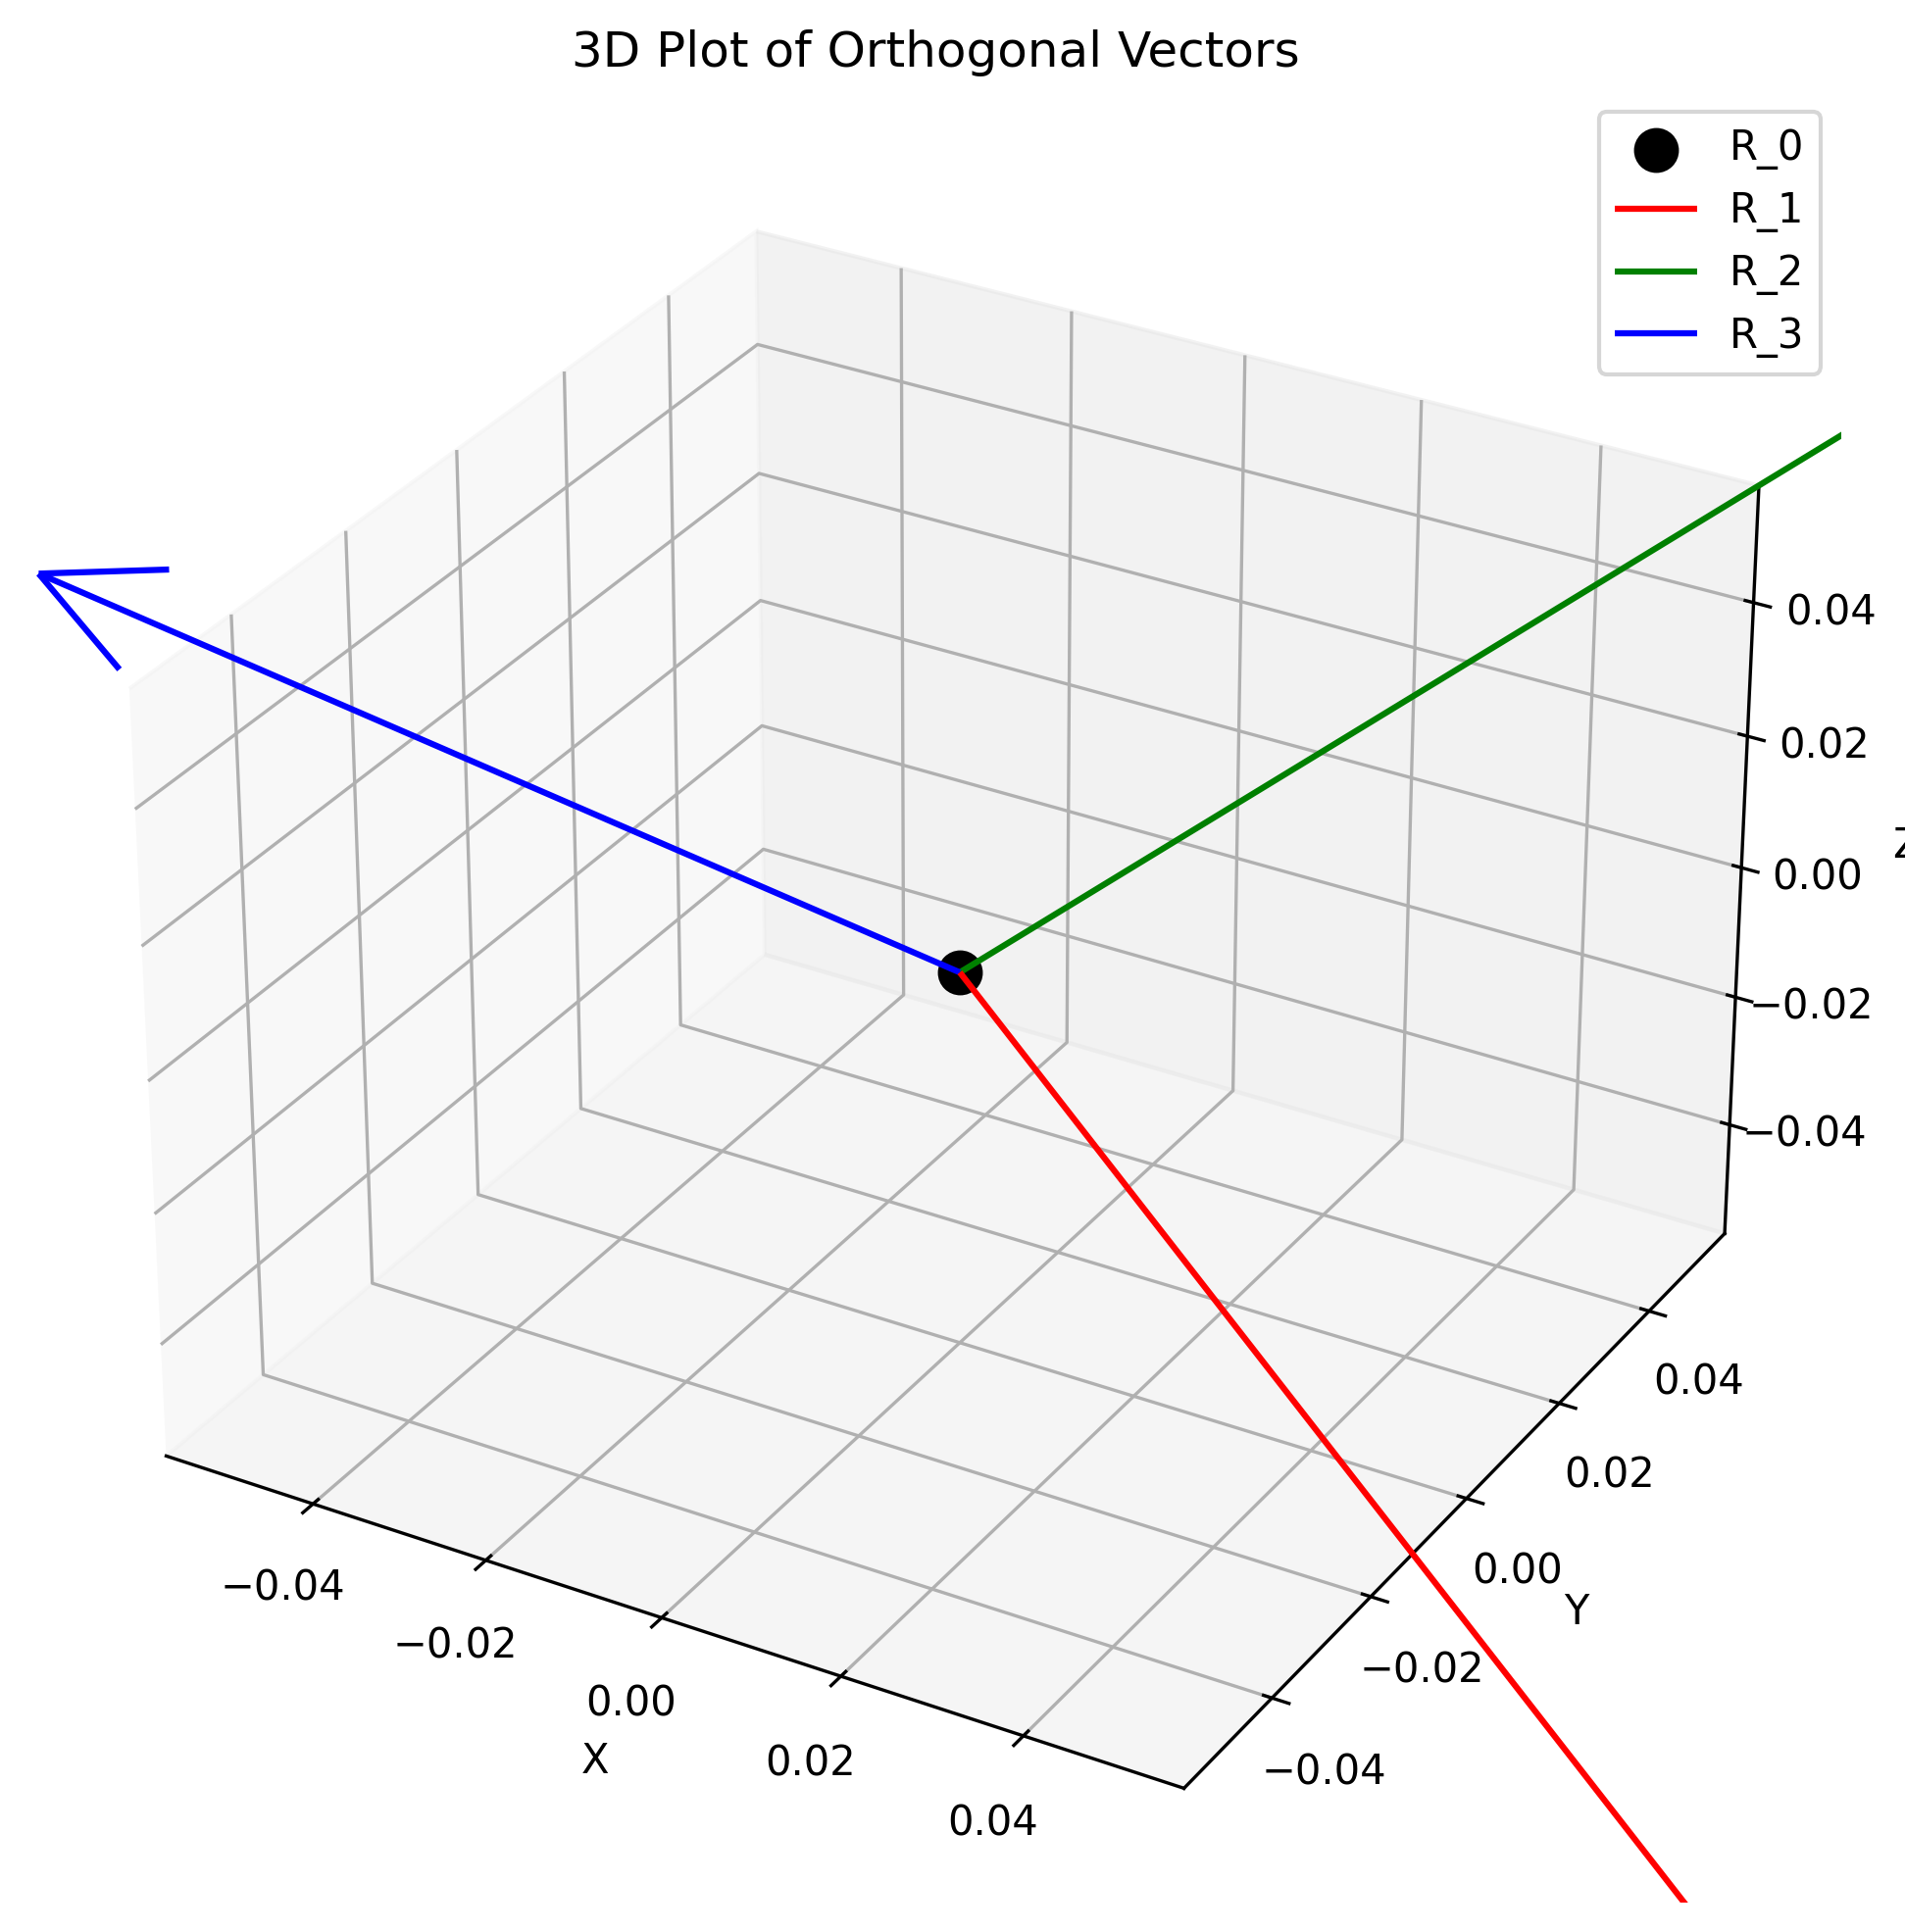
\includegraphics[width=0.8\textwidth]{figures/3d_plot.png}
    \caption{Example of 3D visualization}
    \label{fig:vis_3d_plot}
\end{figure}

\subsection{2D Projections}

The 2D visualization shows projections of the vectors onto various planes. It creates four subplots showing the following projections:

\begin{itemize}
    \item XY Plane: Shows the projection of the vectors onto the XY plane (Z=0).
    \item XZ Plane: Shows the projection of the vectors onto the XZ plane (Y=0).
    \item YZ Plane: Shows the projection of the vectors onto the YZ plane (X=0).
    \item R0 Plane: Shows the projection of the vectors onto the plane perpendicular to the vector from the global origin to $R_0$. This provides a clear view of the orthogonality of the vectors in the plane normal to the origin direction. The projection uses two orthogonal basis vectors in this plane:
        \begin{itemize}
            \item If $R_0$ is the origin (0,0,0), the basis vectors are derived from $R_1$ and $R_2$ after orthogonalization.
            \item Otherwise, the first basis vector is computed as the cross product of the normalized $R_0$ vector with either [1,0,0] or [0,1,0] (whichever is not parallel to $R_0$).
            \item The second basis vector is computed as the cross product of the normalized $R_0$ vector with the first basis vector, ensuring a perfectly orthogonal basis.
        \end{itemize}
\end{itemize}

Each subplot includes the following features:

\begin{itemize}
    \item The origin point is shown as a black dot.
    \item The vectors are shown as arrows from the origin point.
    \item Each vector is assigned a different color for easy identification.
    \item The subplot includes a legend identifying each vector.
    \item The subplot includes labels for the axes.
    \item The subplot includes a title indicating the plane of projection.
\end{itemize}

The 2D projections provide different perspectives on the vectors, allowing for a better understanding of their projections onto different planes.

\begin{figure}[H]
    \centering
    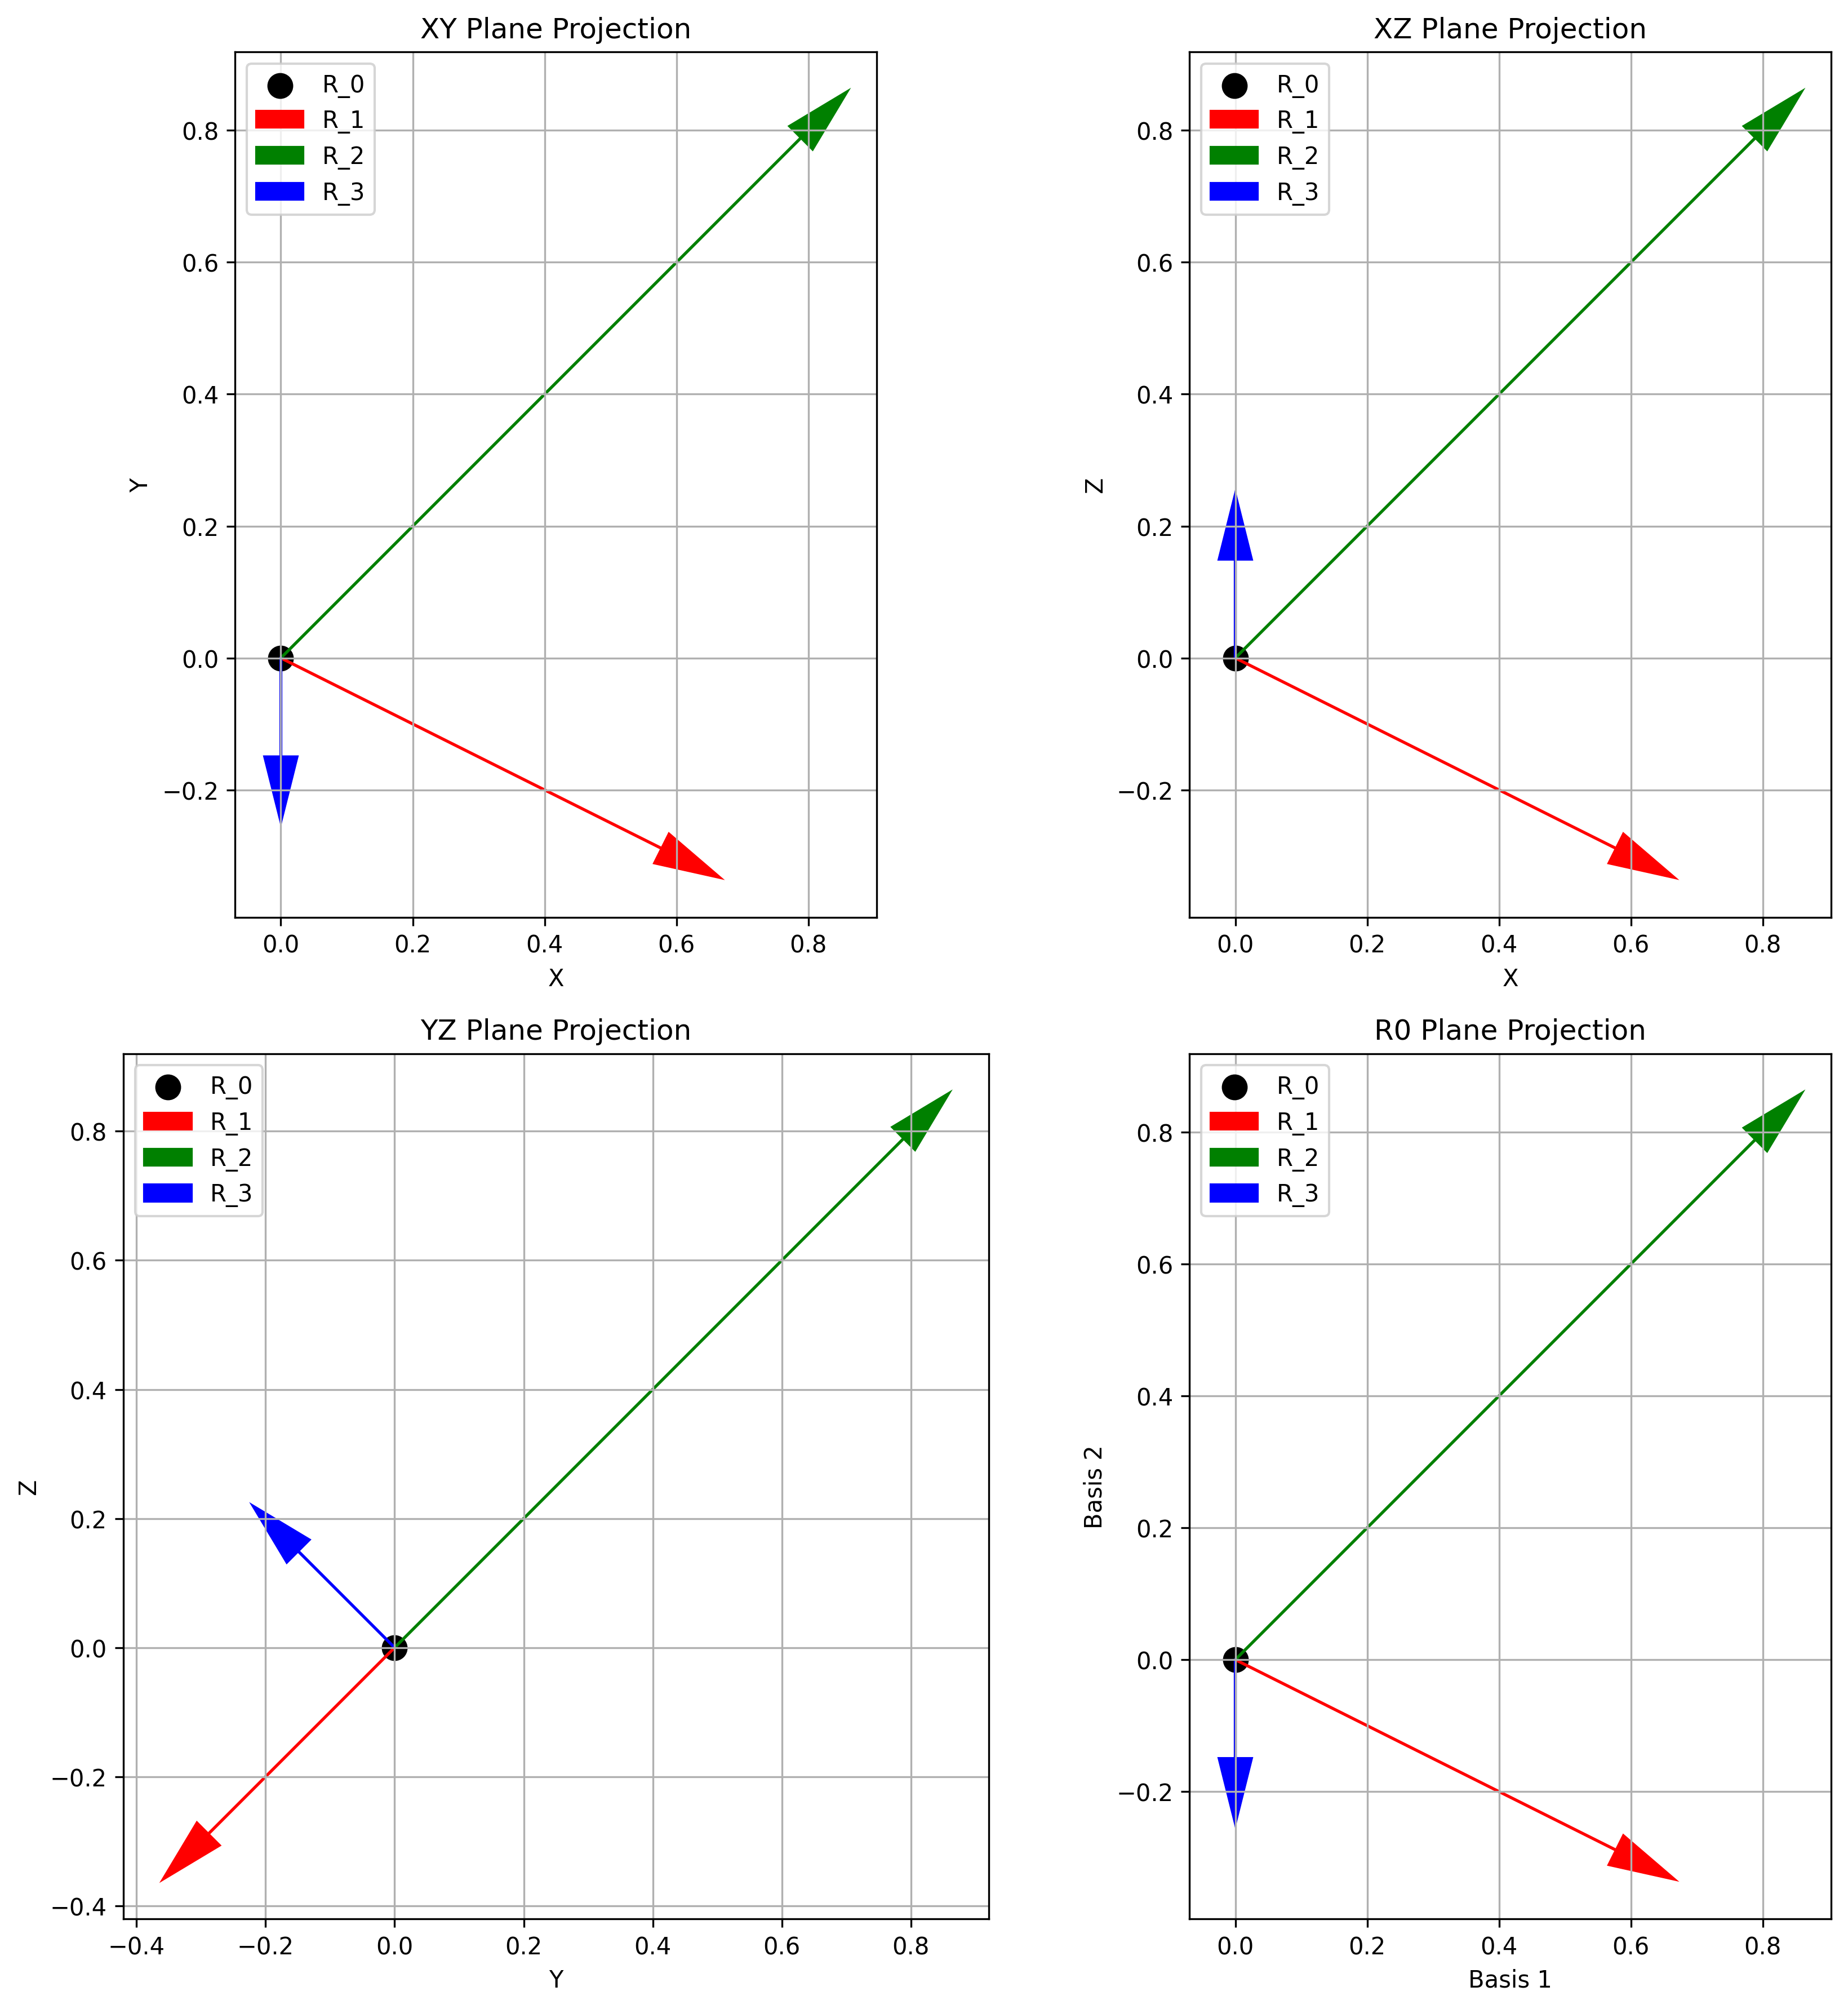
\includegraphics[width=0.8\textwidth]{figures/2d_projections.png}
    \caption{Example of 2D projections}
    \label{fig:vis_2d_projections}
\end{figure}

\subsection{Customization Options}

The visualization functions provide various customization options, including:

\begin{itemize}
    \item Plot title: The title of the plot can be customized.
    \item Show plot: The plot can be displayed interactively or not.
    \item Save path: The plot can be saved to a file instead of being displayed interactively.
\end{itemize}

These options can be specified directly when calling the visualization functions or through the \texttt{VectorConfig} class.

\subsection{R0 Plane Projections}

The package includes specialized scripts for generating R0 plane projections, which provide a clear view of the orthogonality of the vectors in the plane perpendicular to the origin direction:

\begin{itemize}
    \item \texttt{generate\_r0\_projections.py}: Generates R0 plane projections for various configurations with improved axis handling, symmetric axis limits, and better legend placement.
    \item \texttt{generate\_combined\_views.py}: Generates combined 3D and R0 plane projection figures, showing both perspectives side by side.
    \item \texttt{generate\_specific\_r0\_projections.py}: Generates R0 plane projections specifically for the three combined effect configurations (origins at $(0,0,0)$, $(1,1,1)$, and $(0,0,2)$).
\end{itemize}

These projections include the following enhancements:
\begin{itemize}
    \item Dynamic axis limit calculation with a 20\% margin to ensure all vector projections are visible
    \item Symmetric axis limits for better visual representation
    \item Improved grid for better readability
    \item Enhanced legend placement
\end{itemize}

\begin{figure}[H]
    \centering
    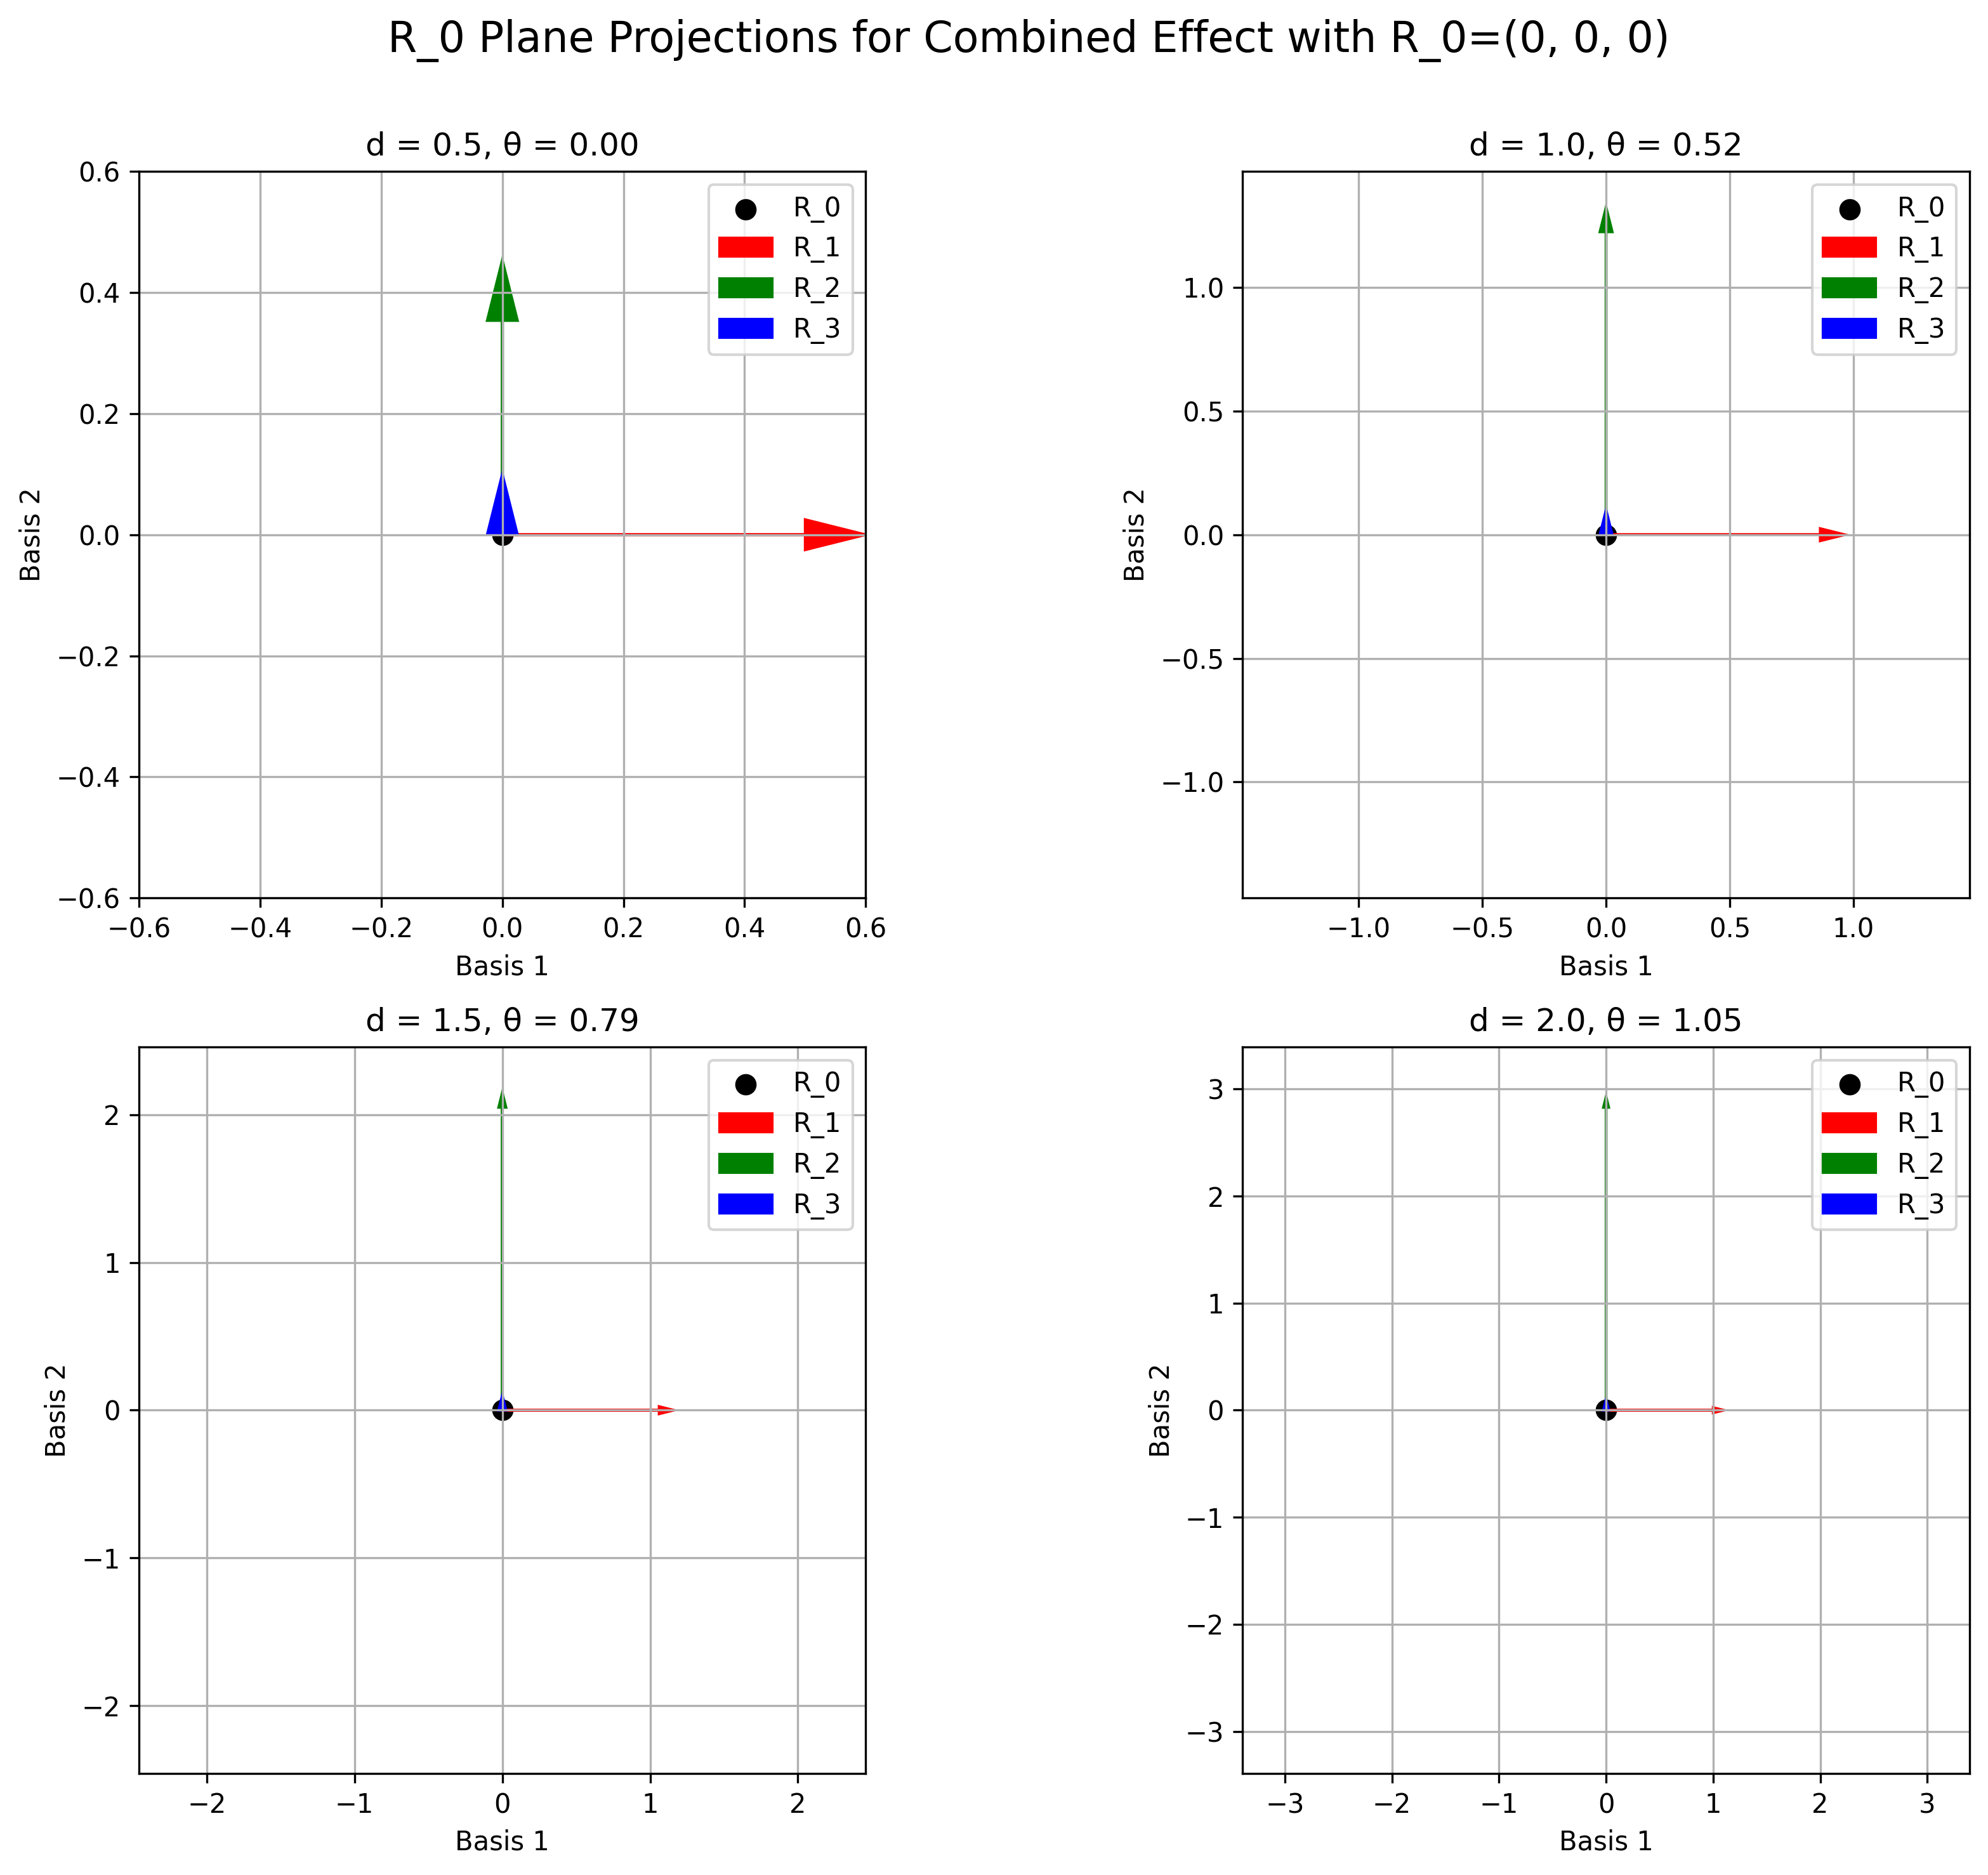
\includegraphics[width=0.8\textwidth]{figures/r0_projections_combined_effect_R0_0_0_0.png}
    \caption{Example of R0 plane projections}
    \label{fig:vis_r0_projections}
\end{figure}

\subsection{Implementation Details}

The visualization functions use Matplotlib to create the plots. The 3D visualization uses Matplotlib's \texttt{Axes3D} class, while the 2D visualizations use regular Matplotlib axes.

The vectors are plotted using Matplotlib's \texttt{quiver} function, which creates arrows from a starting point to an ending point. The origin point is plotted using Matplotlib's \texttt{scatter} function.

The colors of the vectors are assigned using Matplotlib's default color cycle, ensuring that each vector has a different color.

The legends are created using Matplotlib's \texttt{legend} function, with labels for each vector.

The plots are saved using Matplotlib's \texttt{savefig} function, which supports various file formats, including PNG, JPEG, and PDF.

\subsection{Visualization in the Command-line Interface}

The command-line interface provides options for controlling the visualization, including:

\begin{itemize}
    \item \texttt{--plot-type}: Specifies the type of plot, either "3d" or "2d".
    \item \texttt{--title}: Specifies the title of the plot.
    \item \texttt{--no-show}: Prevents the plot from being displayed interactively.
    \item \texttt{--save-path}: Specifies the path to save the plot.
\end{itemize}

These options allow users to customize the visualization without modifying the code.

\newpage
\section{Configuration}

The Generalized Orthogonal Vectors Generator and Visualizer package provides a flexible configuration system that allows users to customize all aspects of vector generation and visualization. This section describes the configuration system and its features.

\subsection{VectorConfig Class}

The configuration system is implemented through the \texttt{VectorConfig} class, which provides a unified way to configure all aspects of vector generation and visualization. The class has the following attributes:

\begin{itemize}
    \item \texttt{origin}: The origin point for vector generation (default: [0, 0, 0]).
    \item \texttt{d}: The distance parameter for vector generation (default: 1.0).
    \item \texttt{theta}: The angle parameter for vector generation (default: $\pi/4$).
    \item \texttt{plot\_type}: The type of plot, either "3d" or "2d" (default: "3d").
    \item \texttt{title}: The title of the plot (default: None, which uses a default title based on the plot type).
    \item \texttt{show\_plot}: Whether to show the plot interactively (default: True).
    \item \texttt{save\_path}: The path to save the plot (default: None, which doesn't save the plot).
    \item \texttt{enhanced\_visualization}: Whether to use enhanced visualization features (default: True).
    \item \texttt{axis\_colors}: Custom colors for the X, Y, and Z axes (default: ['r', 'g', 'b']).
    \item \texttt{show\_coordinate\_labels}: Whether to show coordinate labels on the axes (default: True).
    \item \texttt{equal\_aspect\_ratio}: Whether to maintain an equal aspect ratio for 3D plots (default: True).
\end{itemize}

The class provides methods for initializing the configuration, saving it to a file, and loading it from a file.

\subsection{Initializing a Configuration}

A configuration can be initialized with default values or with custom values:

\begin{lstlisting}[language=Python]
# Initialize with default values
config = VectorConfig()

# Initialize with custom values
config = VectorConfig(
    origin=[1, 1, 1],
    d=2.0,
    theta=math.pi / 3,
    plot_type="2d",
    title="Vector Configuration",
    show_plot=False,
    save_path="custom.png",
    enhanced_visualization=True,
    axis_colors=['red', 'green', 'blue'],
    show_coordinate_labels=True,
    equal_aspect_ratio=True
)
\end{lstlisting}

\subsection{Using a Configuration}

A configuration can be used to generate and visualize orthogonal vectors:

\begin{lstlisting}[language=Python]
# Generate orthogonal vectors using the configuration
vectors = create_orthogonal_vectors(
    origin=config.origin,
    d=config.d,
    theta=config.theta
)

# Plot the vectors using the configuration
plot_vectors(
    vectors,
    origin=config.origin,
    plot_type=config.plot_type,
    title=config.title,
    show_plot=config.show_plot,
    save_path=config.save_path
)
\end{lstlisting}

\subsection{Saving a Configuration to a File}

A configuration can be saved to a JSON file for later use:

\begin{lstlisting}[language=Python]
# Save the configuration to a file
config.save_to_file("config.json")
\end{lstlisting}

The saved file will contain all the configuration parameters in JSON format:

\begin{lstlisting}[language=JSON]
{
    "origin": [1, 1, 1],
    "d": 2.0,
    "theta": 1.0471975511965976,
    "plot_type": "2d",
    "title": "Custom Configuration",
    "show_plot": false,
    "save_path": "custom.png"
}
\end{lstlisting}

\subsection{Loading a Configuration from a File}

A configuration can be loaded from a JSON file:

\begin{lstlisting}[language=Python]
# Load the configuration from a file
config = VectorConfig.load_from_file("config.json")
\end{lstlisting}

This creates a new \texttt{VectorConfig} object with the parameters specified in the file.

\subsection{Configuration in the Command-line Interface}

The command-line interface provides options for configuring vector generation and visualization:

\begin{itemize}
    \item \texttt{--origin}: Specifies the origin point as three space-separated values.
    \item \texttt{--d}: Specifies the distance parameter.
    \item \texttt{--theta}: Specifies the angle parameter in radians.
    \item \texttt{--plot-type}: Specifies the type of plot, either "3d" or "2d".
    \item \texttt{--title}: Specifies the title of the plot.
    \item \texttt{--no-show}: Prevents the plot from being displayed interactively.
    \item \texttt{--save-path}: Specifies the path to save the plot.
    \item \texttt{--config}: Specifies a configuration file to load.
    \item \texttt{--save-config}: Specifies a file to save the configuration to.
    \item \texttt{--no-enhanced-visualization}: Disables enhanced visualization features.
    \item \texttt{--axis-colors}: Specifies custom colors for the X, Y, and Z axes as three space-separated values.
    \item \texttt{--no-coordinate-labels}: Disables coordinate labels on the axes.
    \item \texttt{--no-equal-aspect-ratio}: Disables equal aspect ratio for 3D plots.
\end{itemize}

These options allow users to customize the configuration without modifying the code.

\subsection{Configuration File Format}

The configuration file is a JSON file with the following structure:

\begin{lstlisting}[language=JSON]
{
    "origin": [x, y, z],
    "d": float,
    "theta": float,
    "plot_type": "3d" or "2d",
    "title": string or null,
    "show_plot": boolean,
    "save_path": string or null,
    "enhanced_visualization": boolean,
    "axis_colors": ["r", "g", "b"],
    "show_coordinate_labels": boolean,
    "equal_aspect_ratio": boolean
}
\end{lstlisting}

All fields are optional and will use default values if not specified.

\subsection{Default Configuration}

The default configuration is as follows:

\begin{itemize}
    \item \texttt{origin}: [0, 0, 0]
    \item \texttt{d}: 1.0
    \item \texttt{theta}: $\pi/4$ (approximately 0.7853981633974483)
    \item \texttt{plot\_type}: "3d"
    \item \texttt{title}: None (uses a default title based on the plot type)
    \item \texttt{show\_plot}: True
    \item \texttt{save\_path}: None (doesn't save the plot)
    \item \texttt{enhanced\_visualization}: True
    \item \texttt{axis\_colors}: ['r', 'g', 'b']
    \item \texttt{show\_coordinate\_labels}: True
    \item \texttt{equal\_aspect\_ratio}: True
\end{itemize}

This configuration generates three orthogonal vectors from the origin [0, 0, 0] with a distance parameter of 1.0 and an angle parameter of $\pi/4$, and visualizes them in 3D.

\section{Command-line Interface}

The Generalized Orthogonal Vectors Generator and Visualizer package provides a command-line interface that allows users to generate and visualize orthogonal vectors without writing Python code. This section describes the command-line interface and its features.

\subsection{Basic Usage}

The command-line interface can be accessed by running the \texttt{main.py} module:

\begin{lstlisting}[language=bash]
python -m generalized.main
\end{lstlisting}

This command generates and visualizes orthogonal vectors with default parameters (origin at [0, 0, 0], d=1.0, theta=pi/4).

You can also access detailed help information by running:

\begin{lstlisting}[language=bash]
python -m generalized.main help
\end{lstlisting}

This will display comprehensive information about all available commands, parameters, and usage examples.

\subsection{Command-line Options}

The command-line interface provides various options for configuring vector generation and visualization:

\begin{itemize}
    \item \texttt{--origin X Y Z}, \texttt{-R X Y Z}: Specifies the origin point as three space-separated values. Default: 0 0 0.
    \item \texttt{--distance D}, \texttt{-d D}: Specifies the distance parameter. Default: 1.0.
    \item \texttt{--angle THETA}, \texttt{-a THETA}: Specifies the angle parameter in radians. Default: 0.7853981633974483 (pi/4).
    \item \texttt{--plot-type TYPE}: Specifies the type of plot, either "3d" or "2d". Default: "3d".
    \item \texttt{--title TITLE}: Specifies the title of the plot. Default: None (uses a default title based on the plot type).
    \item \texttt{--no-show}: Prevents the plot from being displayed interactively. Default: False (shows the plot).
    \item \texttt{--save-path PATH}: Specifies the path to save the plot. Default: None (doesn't save the plot).
    \item \texttt{--config FILE}: Specifies a configuration file to load. Default: None (uses command-line options).
    \item \texttt{--save-config FILE}: Specifies a file to save the configuration to. Default: None (doesn't save the configuration).
    \item \texttt{--check-orthogonality}: Checks if the generated vectors are orthogonal and prints the result. Default: False (doesn't check).
    \item \texttt{--verbose}: Enables verbose output, including vector coordinates and dot products. Default: False (minimal output).
    \item \texttt{--help}: Shows the help message and exits.
\end{itemize}

\subsection{Examples}

\subsubsection{Customizing Vector Generation}

\begin{lstlisting}[language=bash]
python -m generalized.main -R 1 1 1 -d 2.0 -a 1.047
\end{lstlisting}

This command generates and visualizes orthogonal vectors with custom parameters (origin at [1, 1, 1], d=2.0, theta=pi/3). Note the use of shorter flags (-R, -d, -a) for more concise commands.

\subsubsection{Customizing Visualization}

\begin{lstlisting}[language=bash]
python -m generalized.main --plot-type 2d --title "Custom Visualization" --save-path custom.png
\end{lstlisting}

This command generates orthogonal vectors with default parameters and visualizes them with custom visualization options (2D plot, custom title, save to file).

\subsubsection{Using a Configuration File}

\begin{lstlisting}[language=bash]
python -m generalized.main --config config.json
\end{lstlisting}

This command loads a configuration from a file and uses it to generate and visualize orthogonal vectors.

\subsubsection{Saving a Configuration File}

\begin{lstlisting}[language=bash]
python -m generalized.main --origin 1 1 1 --d 2.0 --theta 1.047 --save-config config.json
\end{lstlisting}

This command generates and visualizes orthogonal vectors with custom parameters and saves the configuration to a file.

\subsubsection{Checking Orthogonality}

\begin{lstlisting}[language=bash]
python -m generalized.main --check-orthogonality
\end{lstlisting}

This command generates orthogonal vectors with default parameters, visualizes them, and checks if they are orthogonal.

\subsubsection{Verbose Output}

\begin{lstlisting}[language=bash]
python -m generalized.main --verbose
\end{lstlisting}

This command generates orthogonal vectors with default parameters, visualizes them, and prints verbose output, including vector coordinates and dot products.

\subsection{Implementation Details}

The command-line interface is implemented in the \texttt{main.py} module using the \texttt{argparse} module from the Python standard library. The module defines a \texttt{main} function that parses command-line arguments, creates a configuration, generates orthogonal vectors, and visualizes them.

The command-line interface follows these steps:

\begin{enumerate}
    \item Parse command-line arguments using \texttt{argparse}.
    \item If a configuration file is specified, load the configuration from the file.
    \item Override the configuration with any command-line options that are specified.
    \item Generate orthogonal vectors using the configuration.
    \item If requested, check if the vectors are orthogonal and print the result.
    \item If verbose output is enabled, print vector coordinates and dot products.
    \item Visualize the vectors using the configuration.
    \item If requested, save the configuration to a file.
\end{enumerate}

\subsection{Error Handling}

The command-line interface includes error handling for various scenarios, including:

\begin{itemize}
    \item Invalid command-line arguments (e.g., non-numeric values for numeric options).
    \item Invalid configuration file (e.g., file not found, invalid JSON).
    \item Invalid configuration parameters (e.g., negative distance parameter).
\end{itemize}

When an error occurs, the command-line interface prints an error message and exits with a non-zero exit code.

\subsection{Help Message}

The command-line interface provides a help message that can be displayed using the \texttt{--help} option:

\begin{lstlisting}[language=bash]
python -m generalized.main --help
\end{lstlisting}

The help message includes a description of the program, a list of all available options, and examples of how to use the program.

\section{Example Results}

This section presents example results for different configurations of the Generalized Orthogonal Vectors Generator and Visualizer. It shows the generated vectors and their visualizations for various parameter values.

\subsection{Default Configuration}

The default configuration generates three orthogonal vectors from the origin [0, 0, 0] with a distance parameter of 1.0 and an angle parameter of $\pi/4$.

\subsubsection{Vector Coordinates}

The coordinates of the generated vectors are:

\begin{align}
\vec{R}_1 &= \begin{pmatrix} 0.8165 \\ -0.4082 \\ -0.4082 \end{pmatrix} \\
\vec{R}_2 &= \begin{pmatrix} 0.5774 \\ 0.5774 \\ 0.5774 \end{pmatrix} \\
\vec{R}_3 &= \begin{pmatrix} 0 \\ -0.7071 \\ 0.7071 \end{pmatrix}
\end{align}

\subsubsection{Dot Products}

The dot products between the displacement vectors are:

\begin{align}
\vec{v}_1 \cdot \vec{v}_2 &= 0 \\
\vec{v}_1 \cdot \vec{v}_3 &= 0 \\
\vec{v}_2 \cdot \vec{v}_3 &= 0
\end{align}

These dot products confirm that the vectors are orthogonal.

\subsubsection{3D Visualization}

\begin{figure}[H]
    \centering
    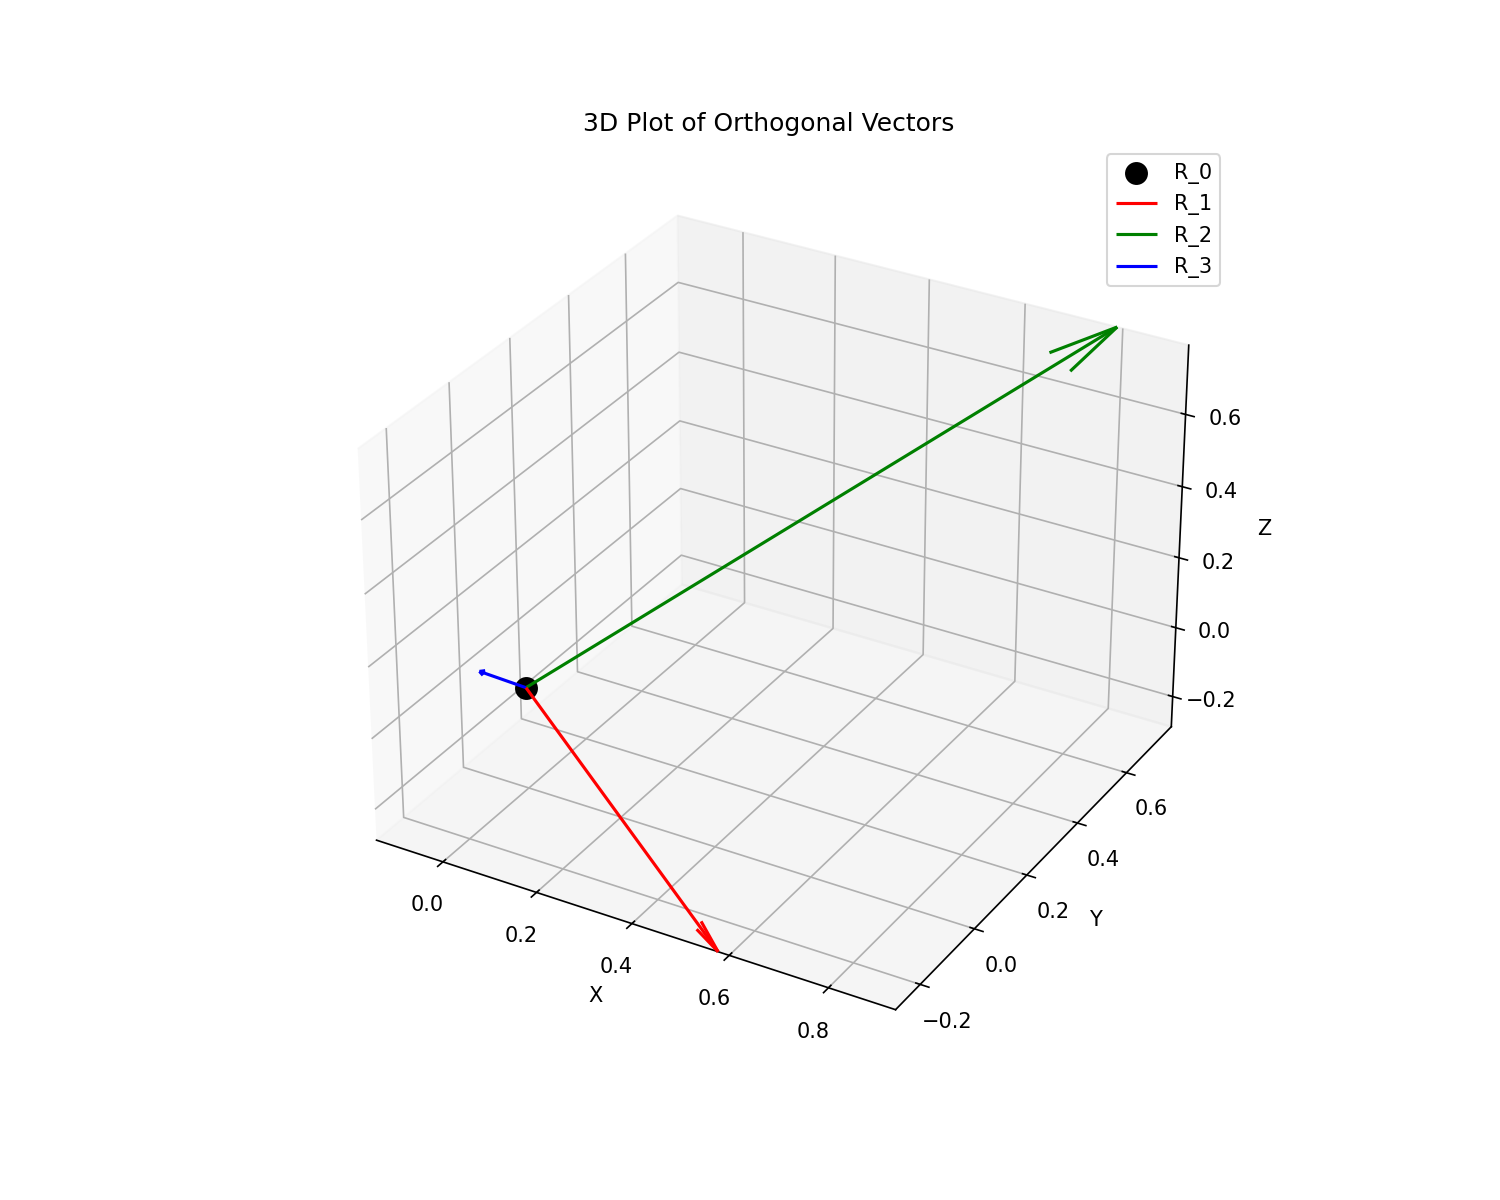
\includegraphics[width=0.8\textwidth]{figures/default_3d.png}
    \caption{3D visualization of the default configuration}
    \label{fig:example_default_3d}
\end{figure}

\subsubsection{2D Projections}

\begin{figure}[H]
    \centering
    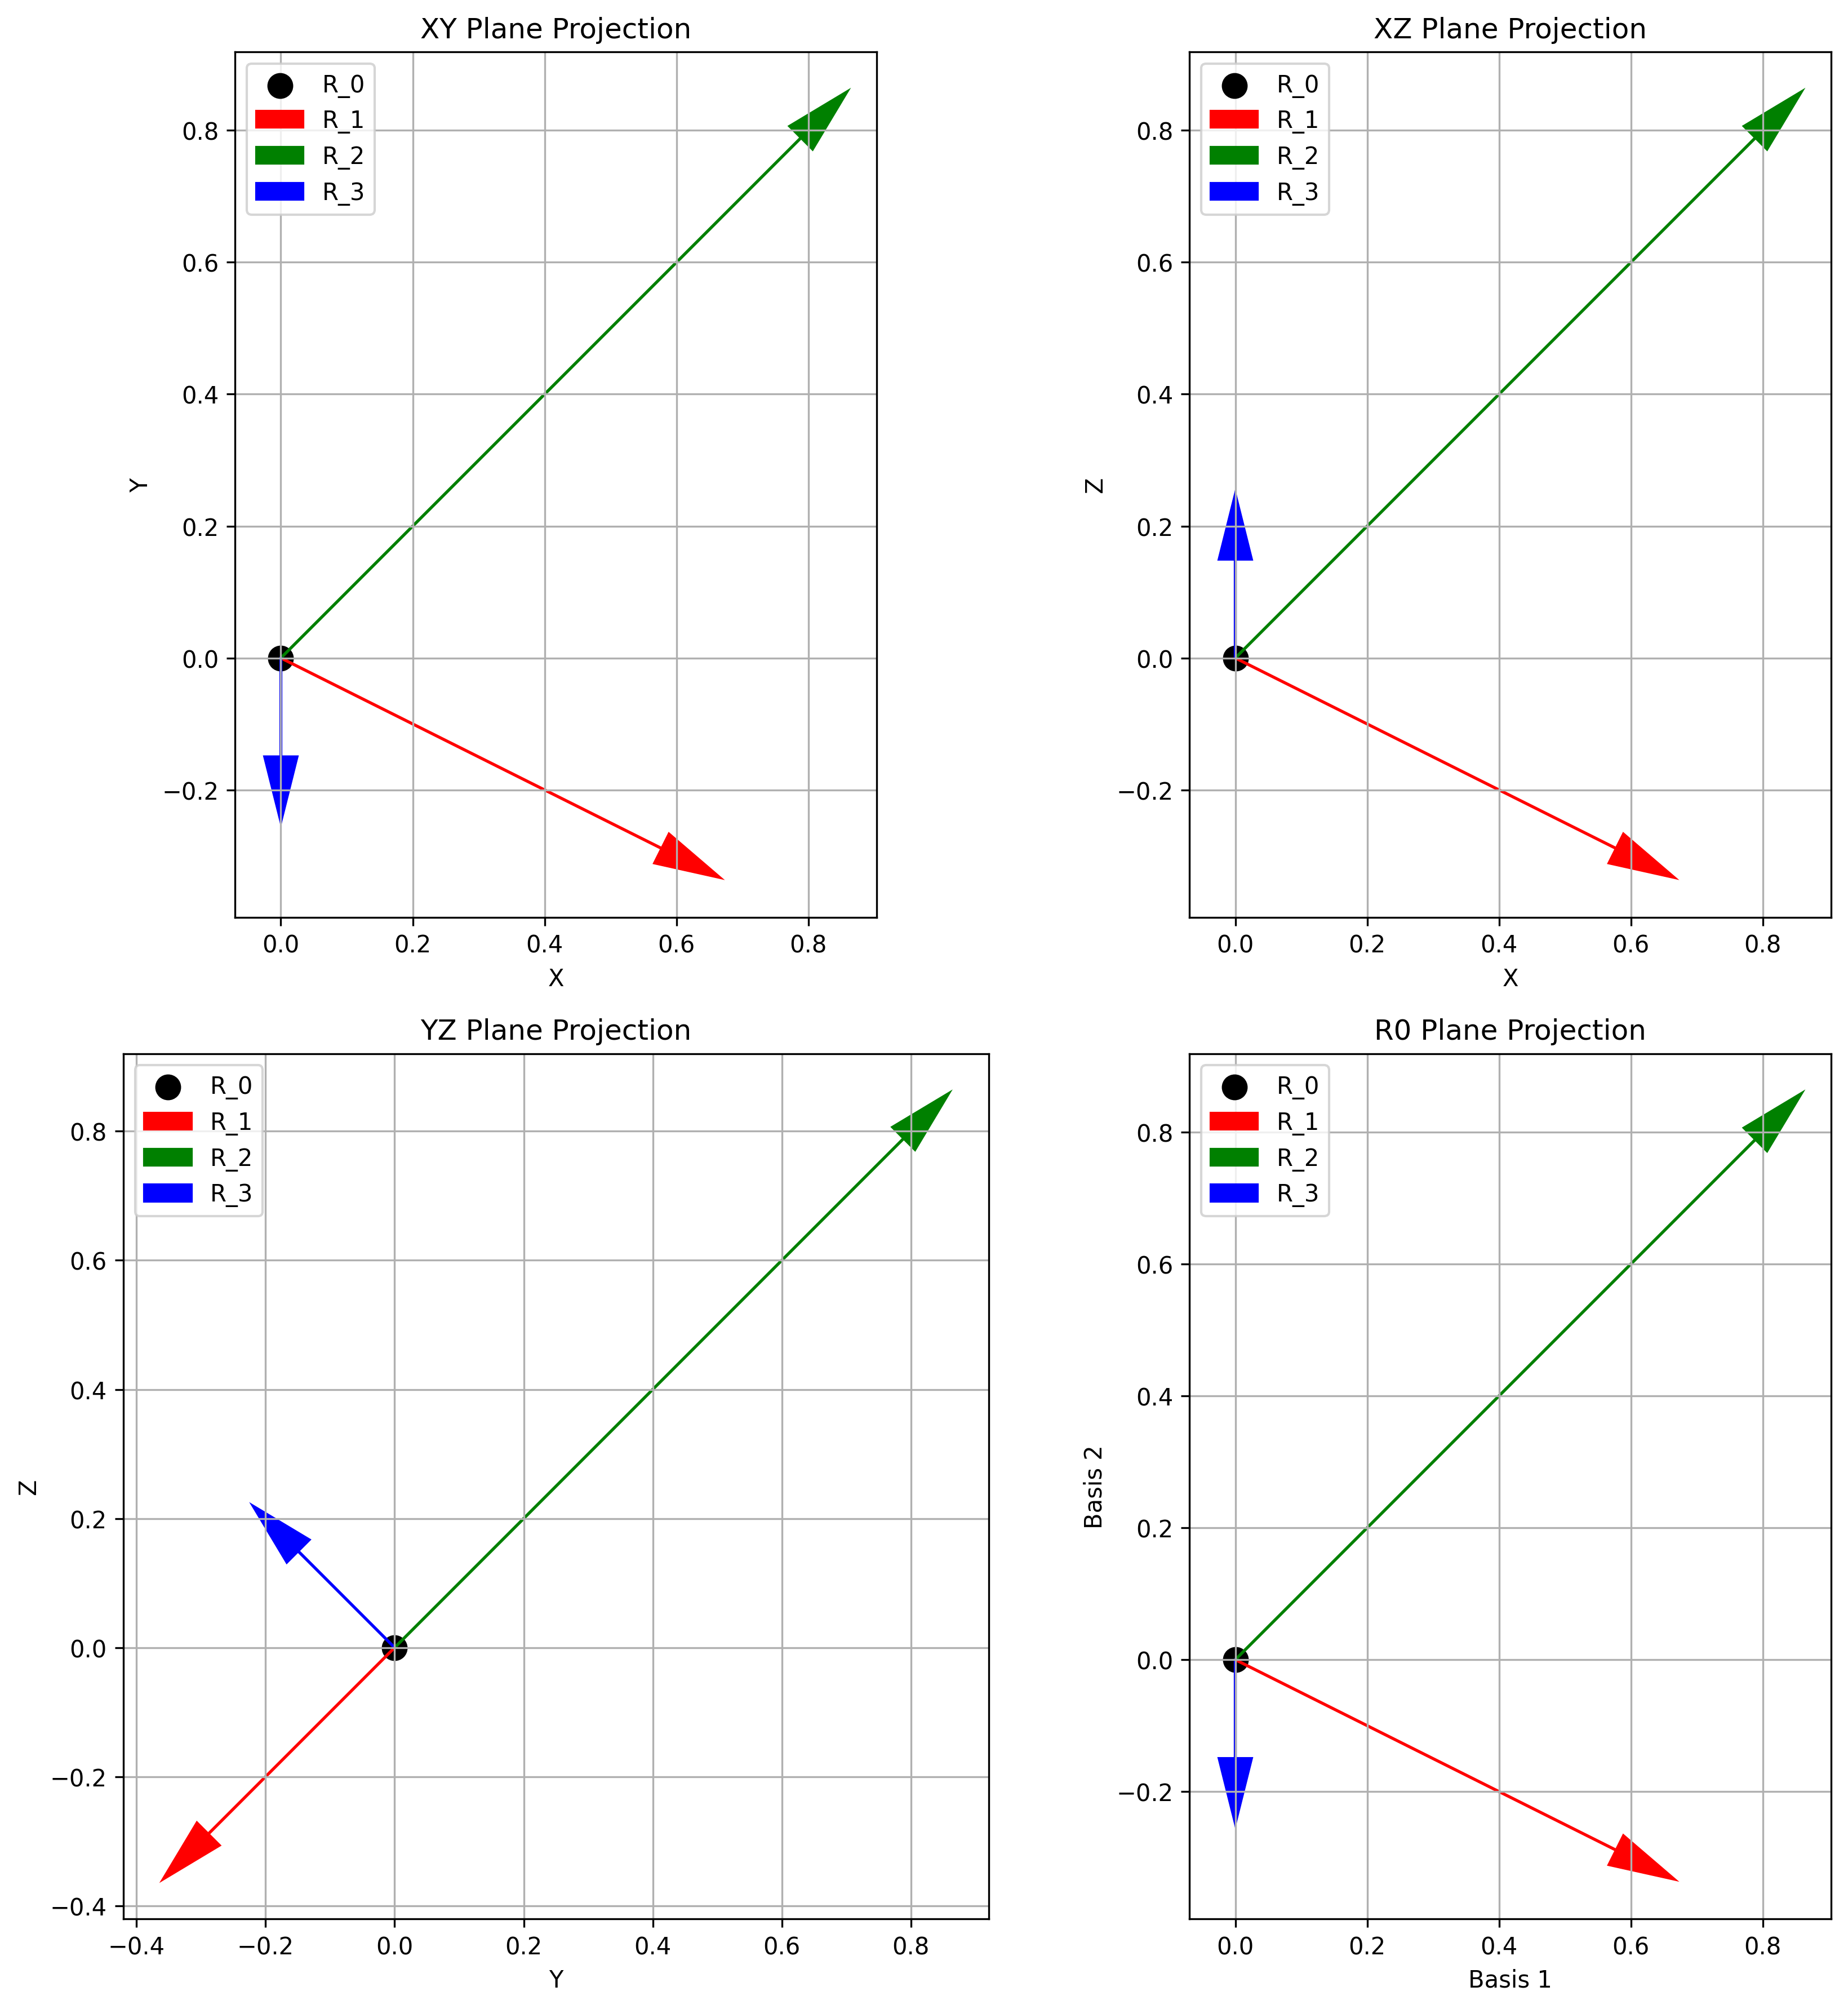
\includegraphics[width=0.8\textwidth]{figures/2d_projections.png}
    \caption{2D projections of the default configuration}
    \label{fig:example_default_2d}
\end{figure}

\subsection{Custom Configuration 1}

This configuration generates three orthogonal vectors from the origin [1, 1, 1] with a distance parameter of 2.0 and an angle parameter of $\pi/3$.

\subsubsection{Vector Coordinates}

The coordinates of the generated vectors are:

\begin{align}
\vec{R}_1 &= \begin{pmatrix} 2.6330 \\ 0.3165 \\ 0.3165 \end{pmatrix} \\
\vec{R}_2 &= \begin{pmatrix} 1.6667 \\ 1.6667 \\ 1.6667 \end{pmatrix} \\
\vec{R}_3 &= \begin{pmatrix} 1 \\ -0.1547 \\ 2.1547 \end{pmatrix}
\end{align}

\subsubsection{Dot Products}

The dot products between the displacement vectors are:

\begin{align}
\vec{v}_1 \cdot \vec{v}_2 &= 0 \\
\vec{v}_1 \cdot \vec{v}_3 &= 0 \\
\vec{v}_2 \cdot \vec{v}_3 &= 0
\end{align}

These dot products confirm that the vectors are orthogonal.

\subsubsection{3D Visualization}

\begin{figure}[H]
    \centering
    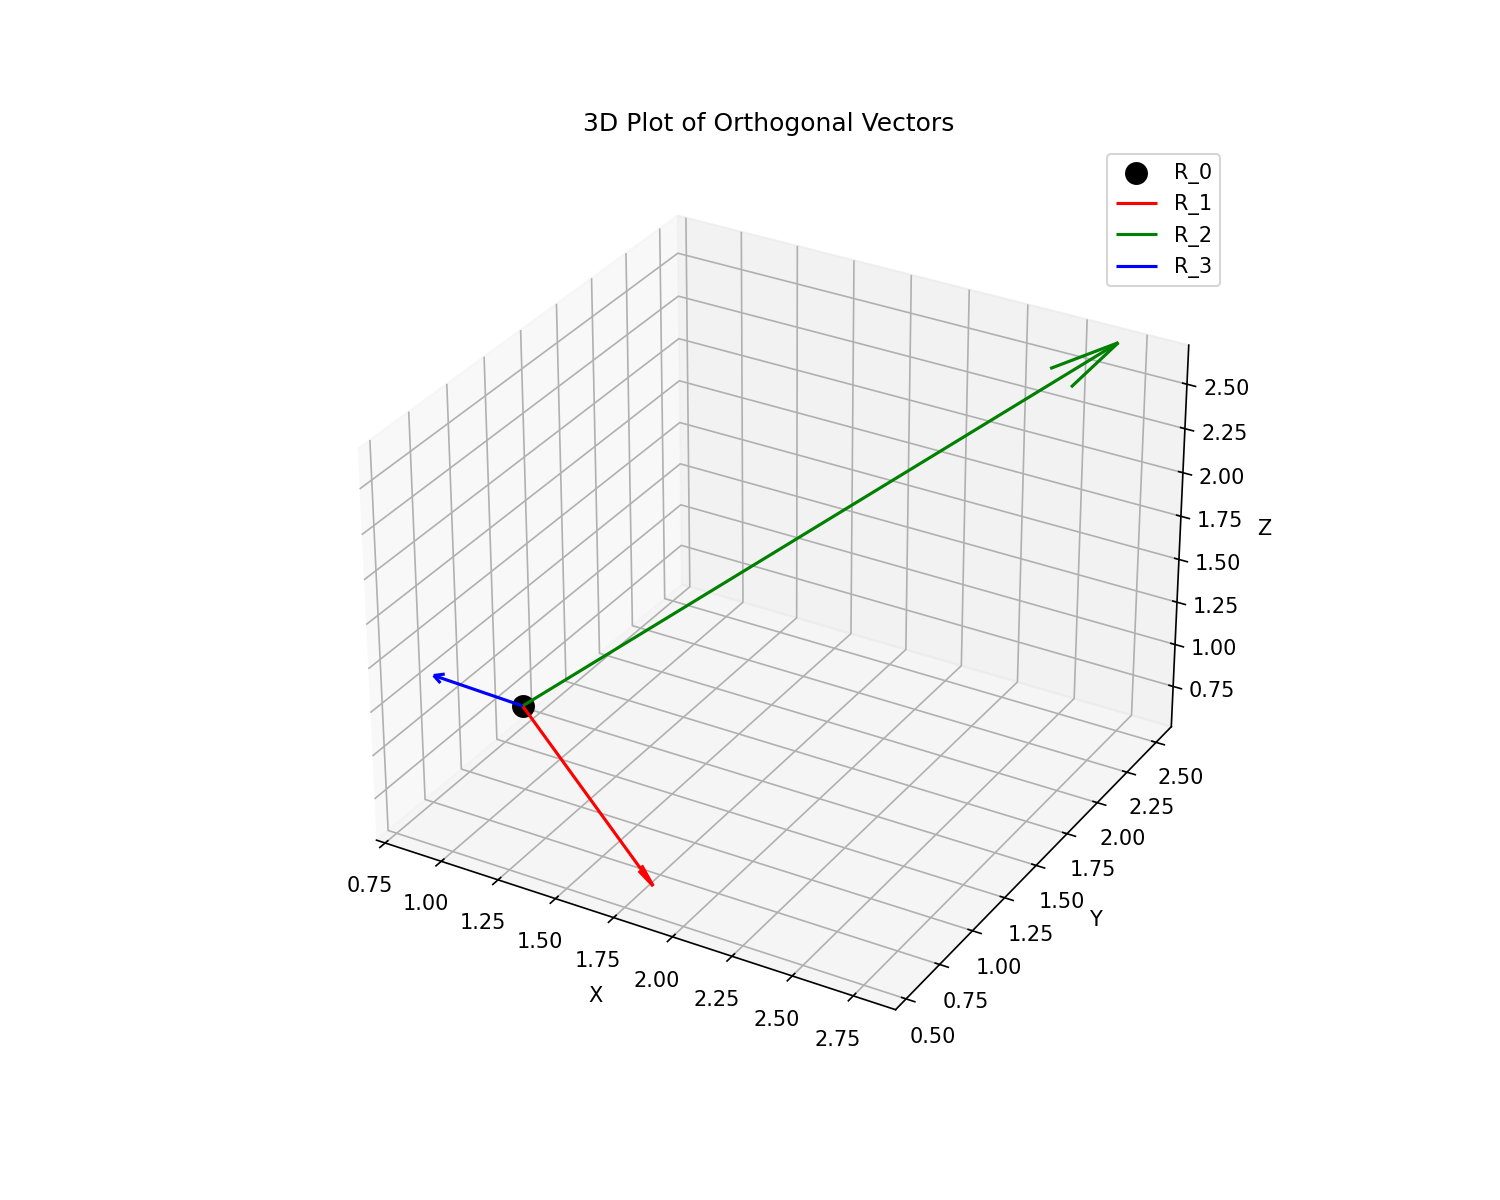
\includegraphics[width=0.8\textwidth]{figures/custom1_3d.png}
    \caption{3D visualization of custom configuration 1}
    \label{fig:example_custom1_3d}
\end{figure}

\subsubsection{2D Projections}

\begin{figure}[H]
    \centering
    \begin{minipage}{0.48\textwidth}
        \centering
        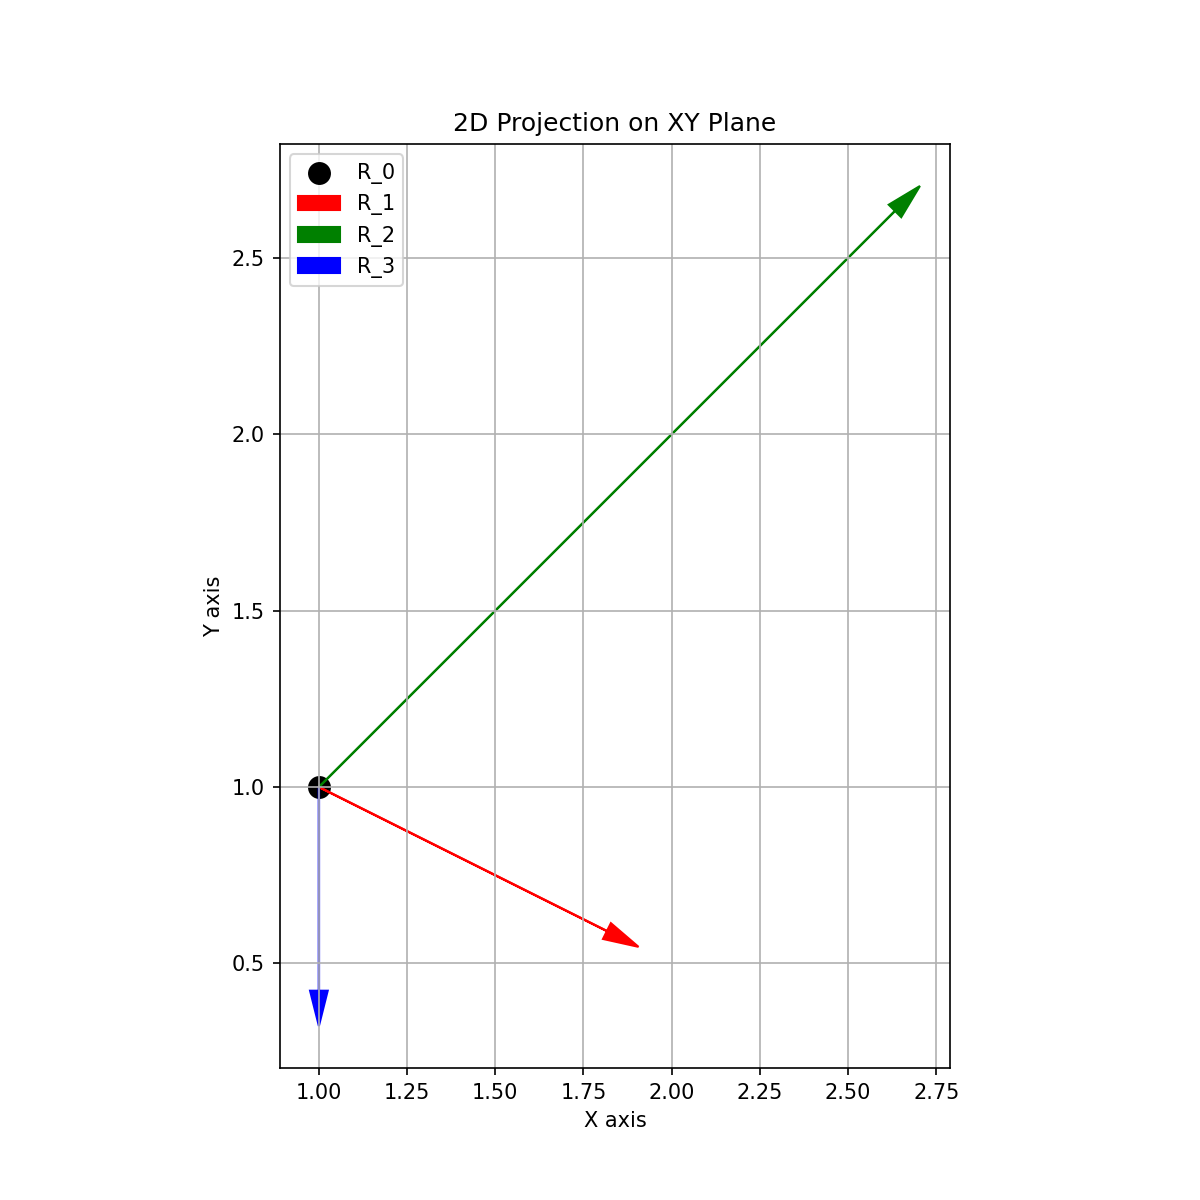
\includegraphics[width=\textwidth]{figures/custom1_xy.png}
        \caption*{XY Projection}
    \end{minipage}\hfill
    \begin{minipage}{0.48\textwidth}
        \centering
        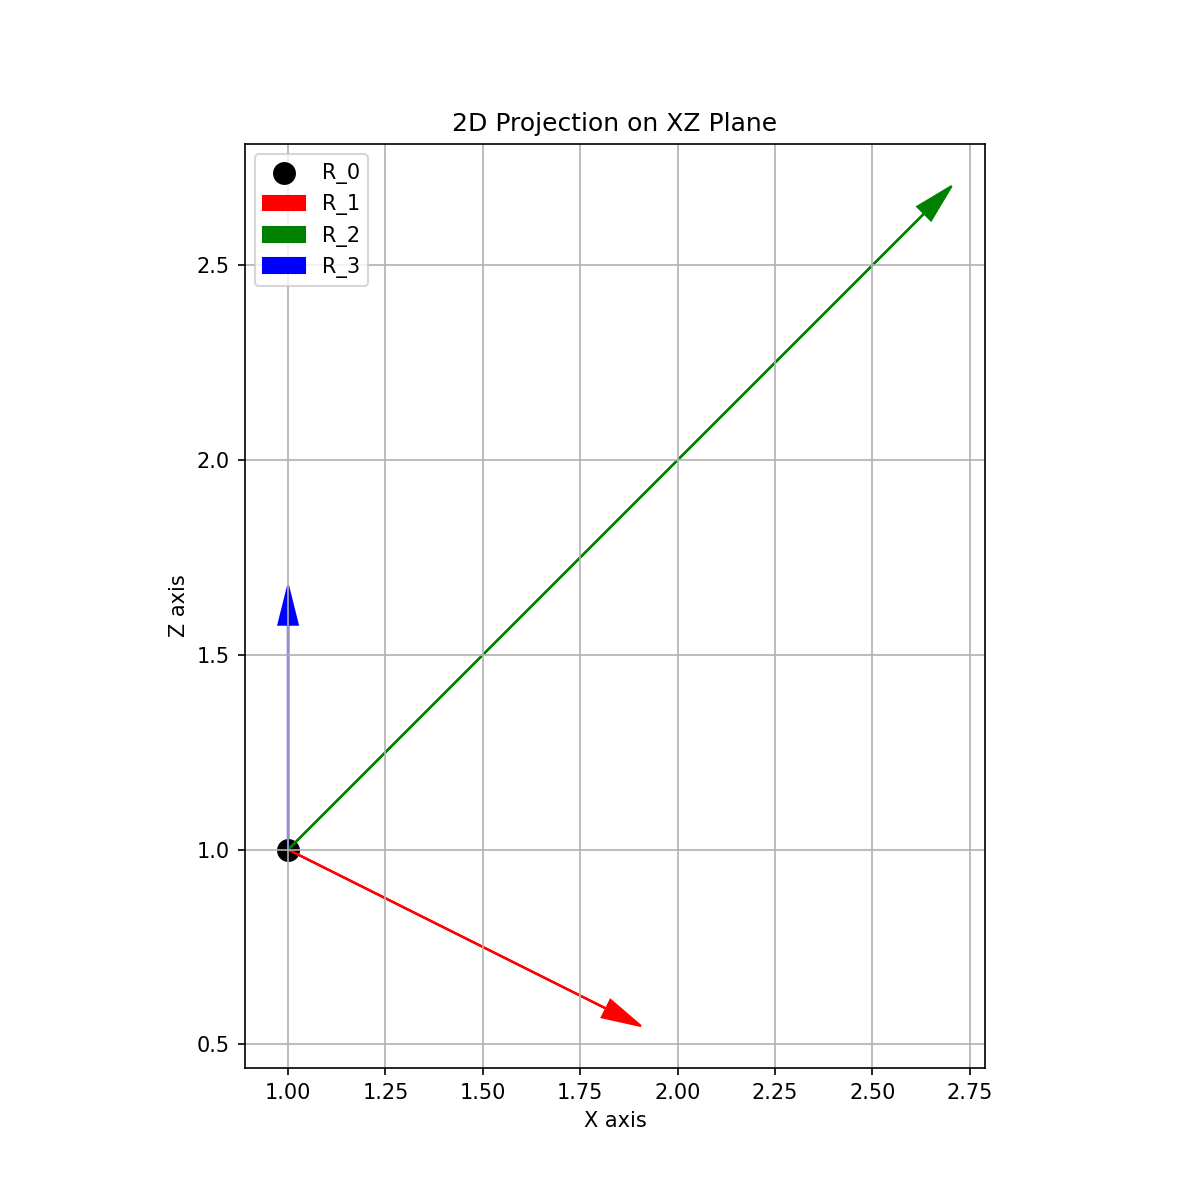
\includegraphics[width=\textwidth]{figures/custom1_xz.png}
        \caption*{XZ Projection}
    \end{minipage}
    
    \begin{minipage}{0.48\textwidth}
        \centering
        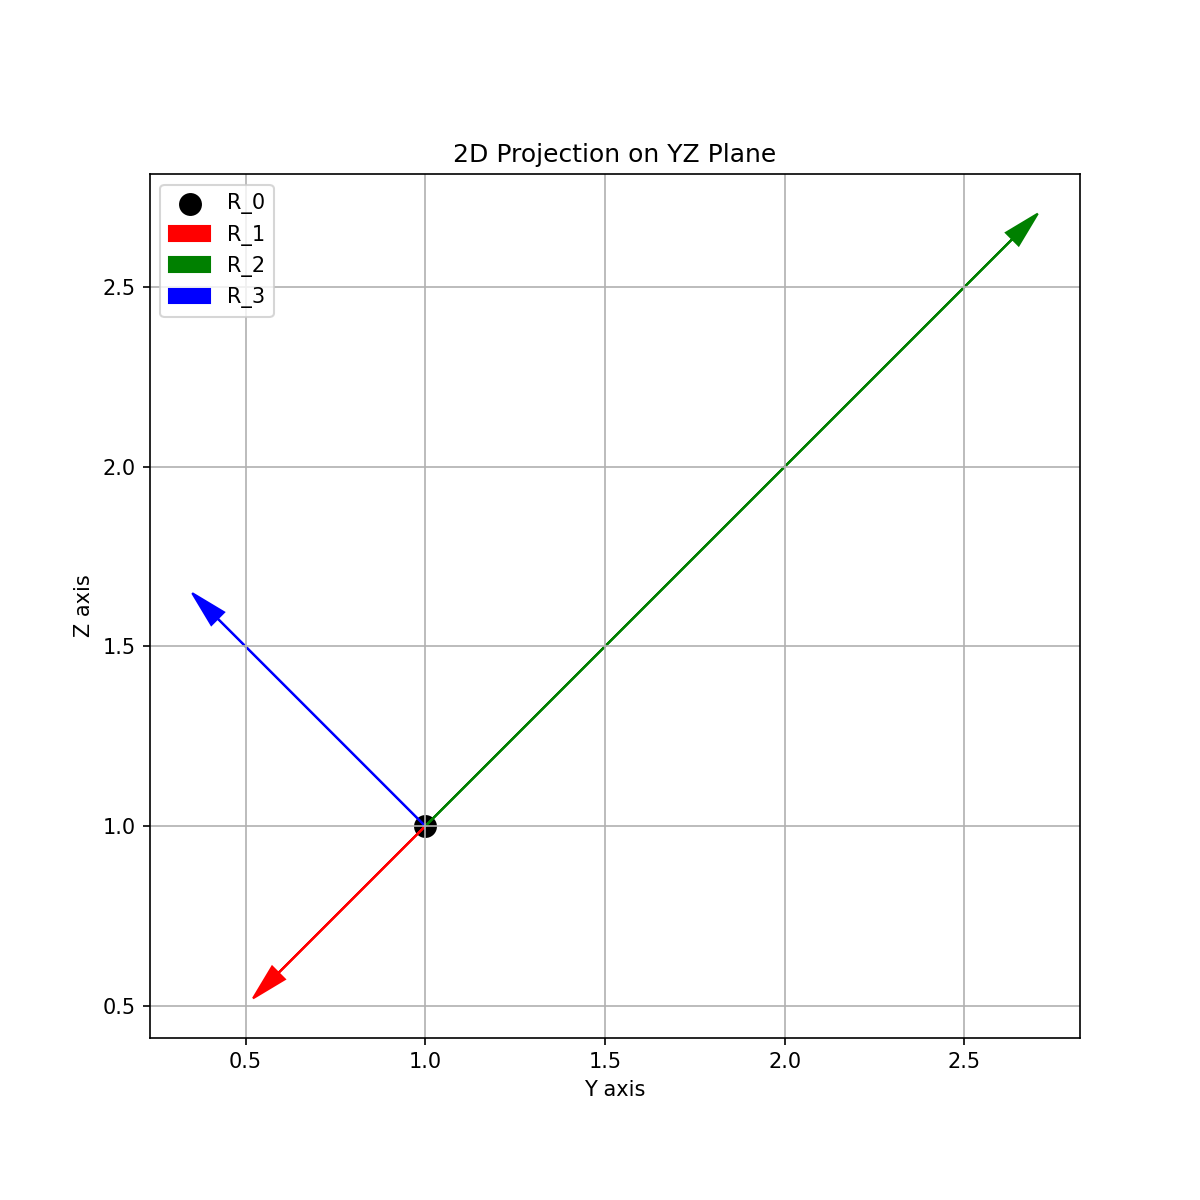
\includegraphics[width=\textwidth]{figures/custom1_yz.png}
        \caption*{YZ Projection}
    \end{minipage}\hfill
    \begin{minipage}{0.48\textwidth}
        \centering
        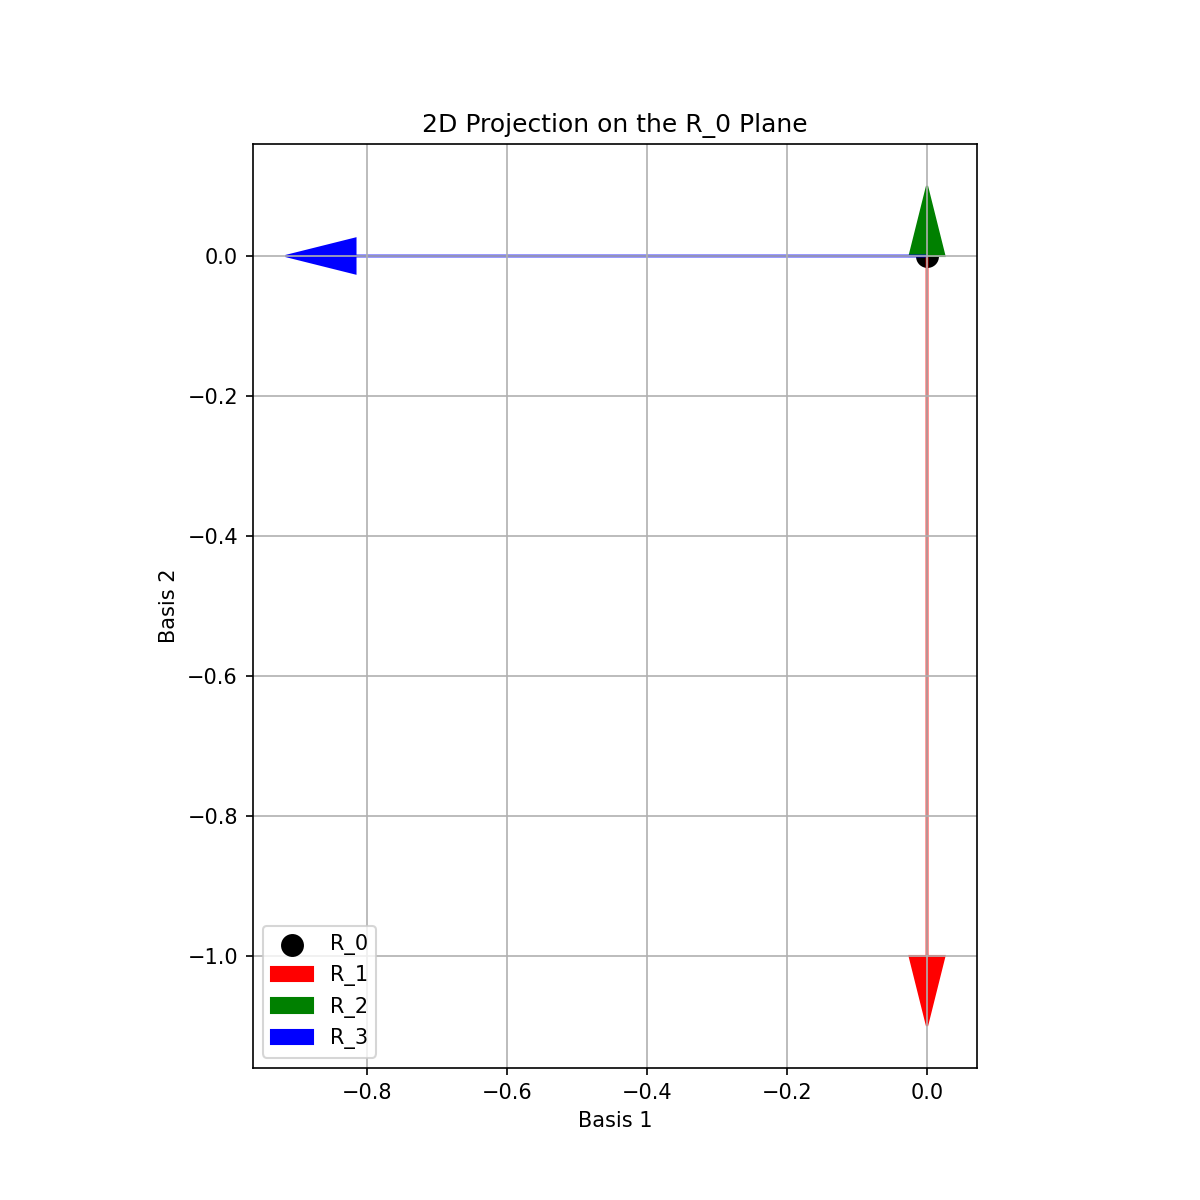
\includegraphics[width=\textwidth]{figures/custom1_r0.png}
        \caption*{R0 Projection}
    \end{minipage}
    \caption{2D projections of custom configuration 1}
    \label{fig:example_custom1_2d}
\end{figure}

\subsection{Custom Configuration 2}

This configuration generates three orthogonal vectors from the origin [0, 0, 2] with a distance parameter of 1.5 and an angle parameter of $\pi/6$.

\subsubsection{Vector Coordinates}

The coordinates of the generated vectors are:

\begin{align}
\vec{R}_1 &= \begin{pmatrix} 1.2990 \\ -0.6495 \\ 1.3505 \end{pmatrix} \\
\vec{R}_2 &= \begin{pmatrix} 0.7217 \\ 0.7217 \\ 2.7217 \end{pmatrix} \\
\vec{R}_3 &= \begin{pmatrix} 0 \\ -0.3750 \\ 2.3750 \end{pmatrix}
\end{align}

\subsubsection{Dot Products}

The dot products between the displacement vectors are:

\begin{align}
\vec{v}_1 \cdot \vec{v}_2 &= 0 \\
\vec{v}_1 \cdot \vec{v}_3 &= 0 \\
\vec{v}_2 \cdot \vec{v}_3 &= 0
\end{align}

These dot products confirm that the vectors are orthogonal.

\subsubsection{3D Visualization}

\begin{figure}[H]
    \centering
    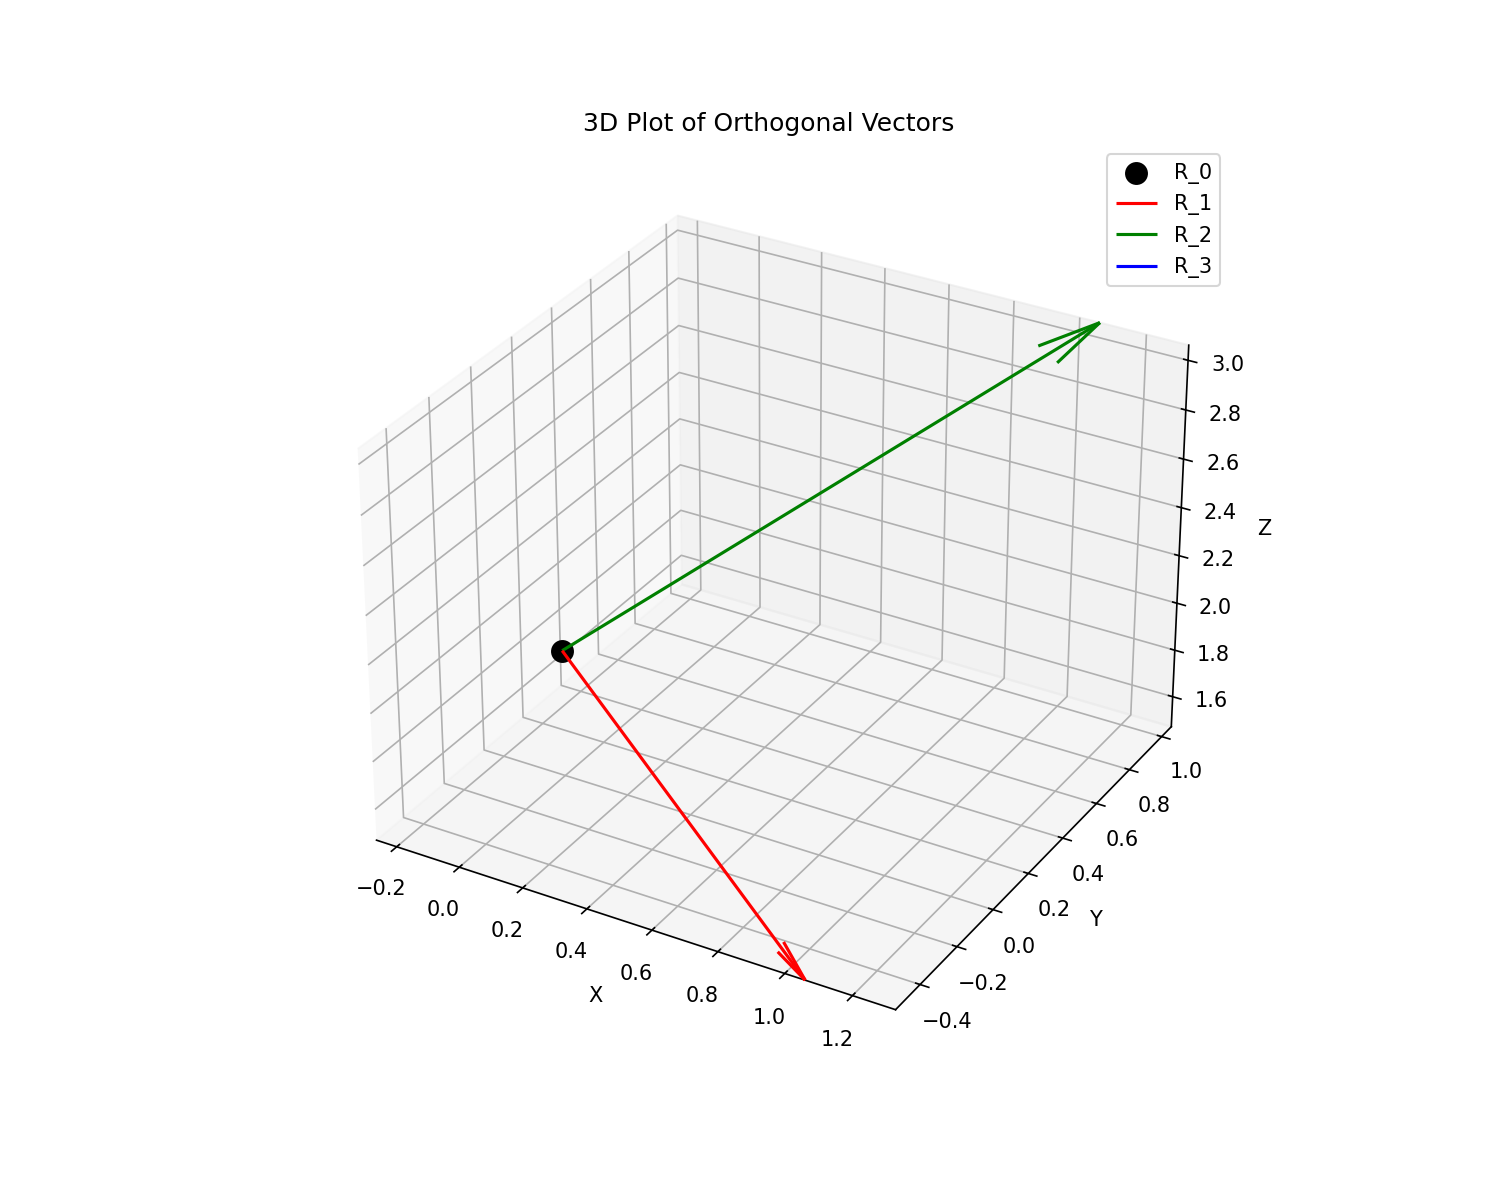
\includegraphics[width=0.8\textwidth]{figures/custom2_3d.png}
    \caption{3D visualization of custom configuration 2}
    \label{fig:example_custom2_3d}
\end{figure}

\subsubsection{2D Projections}

\begin{figure}[H]
    \centering
    \begin{minipage}{0.48\textwidth}
        \centering
        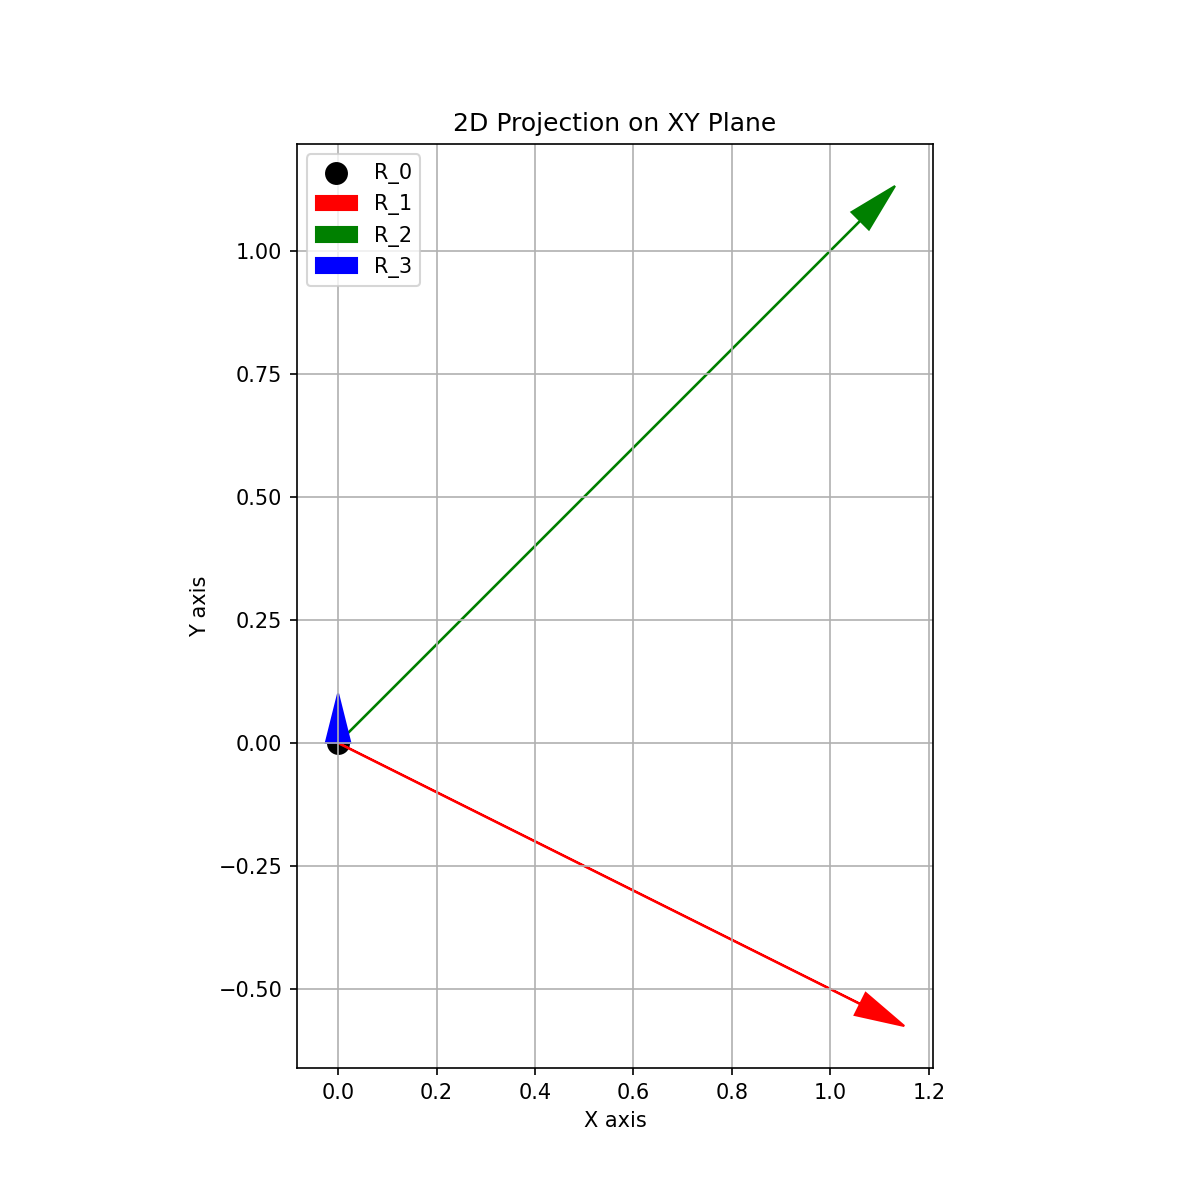
\includegraphics[width=\textwidth]{figures/custom2_xy.png}
        \caption*{XY Projection}
    \end{minipage}\hfill
    \begin{minipage}{0.48\textwidth}
        \centering
        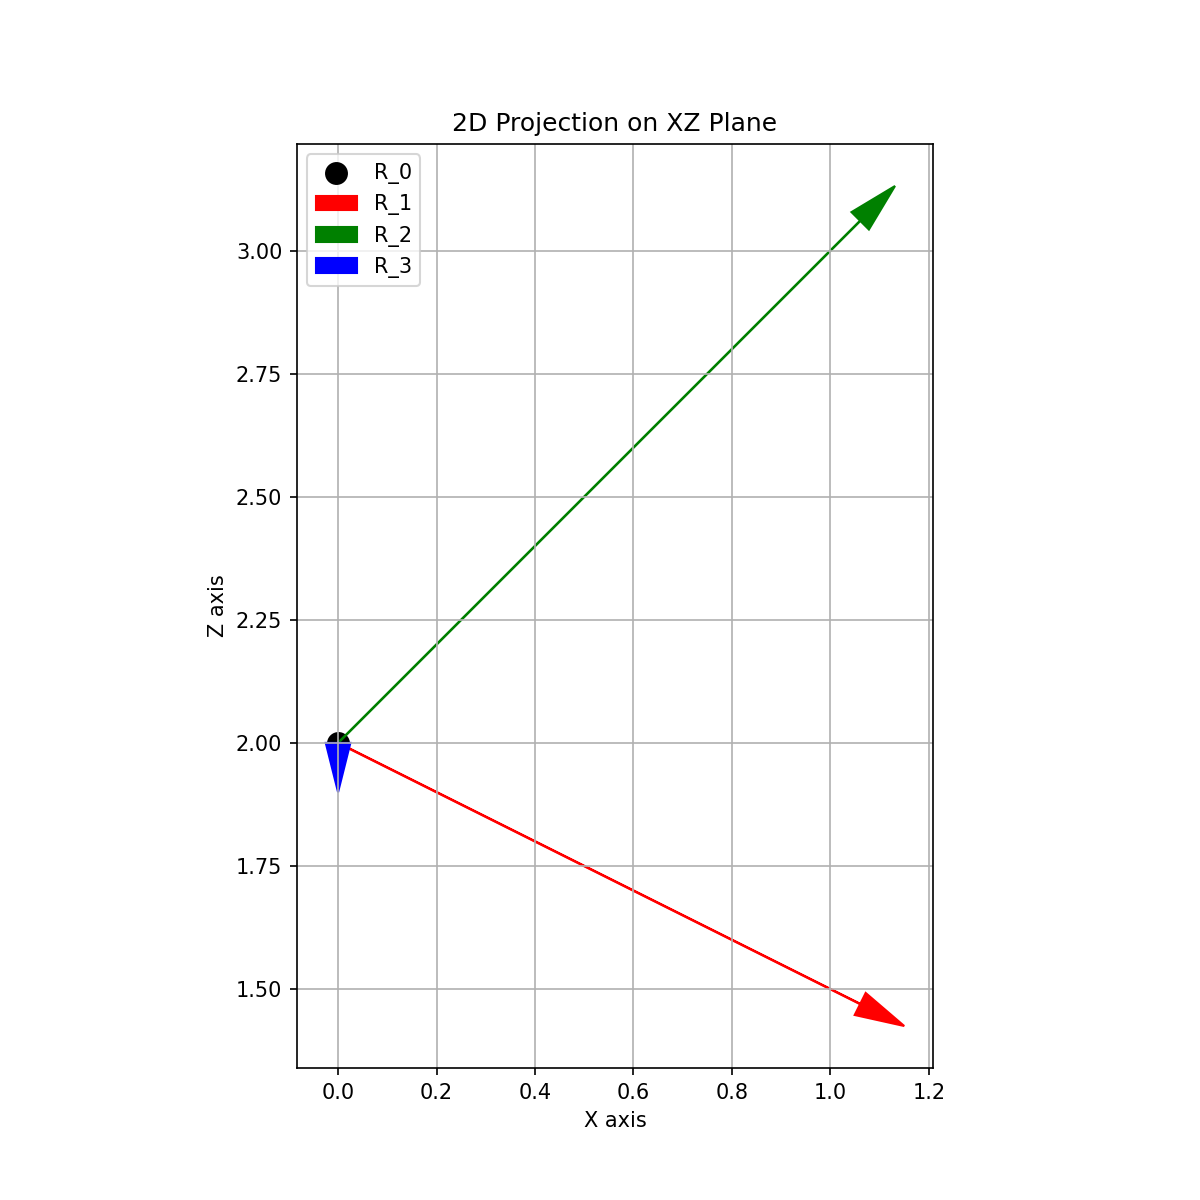
\includegraphics[width=\textwidth]{figures/custom2_xz.png}
        \caption*{XZ Projection}
    \end{minipage}
    
    \begin{minipage}{0.48\textwidth}
        \centering
        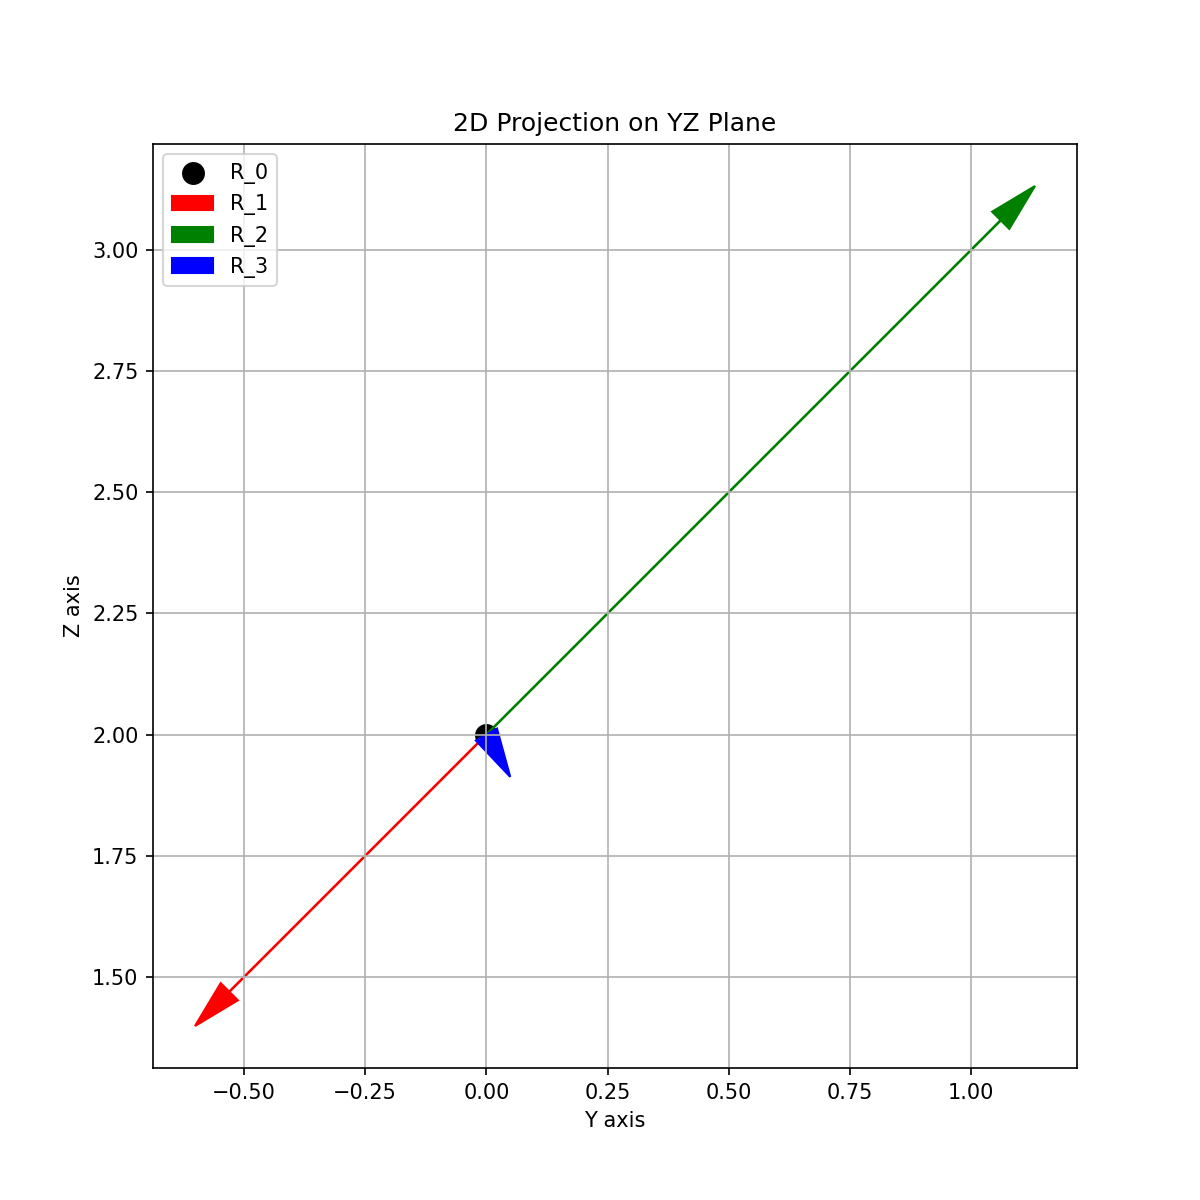
\includegraphics[width=\textwidth]{figures/custom2_yz.png}
        \caption*{YZ Projection}
    \end{minipage}\hfill
    \begin{minipage}{0.48\textwidth}
        \centering
        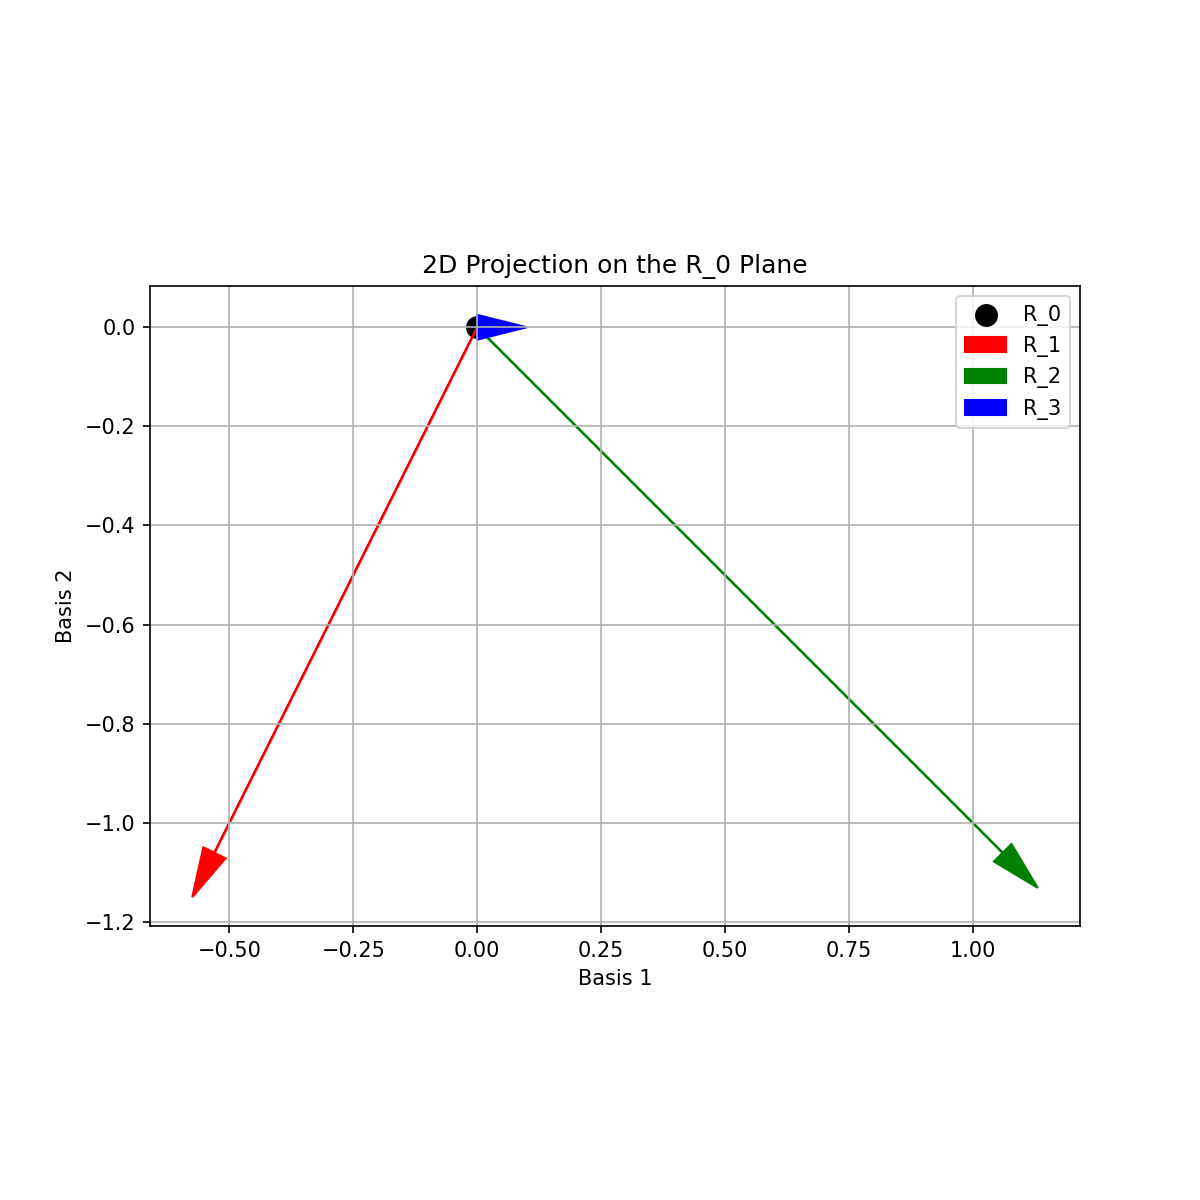
\includegraphics[width=\textwidth]{figures/custom2_r0.png}
        \caption*{R0 Projection}
    \end{minipage}
    \caption{2D projections of custom configuration 2}
    \label{fig:example_custom2_2d}
\end{figure}

\subsection{Effect of Distance Parameter}

The distance parameter $d$ scales the vectors equally, preserving their orthogonality. Increasing $d$ increases the distance of the vectors from the origin, while decreasing $d$ decreases the distance.

\begin{figure}[H]
    \centering
    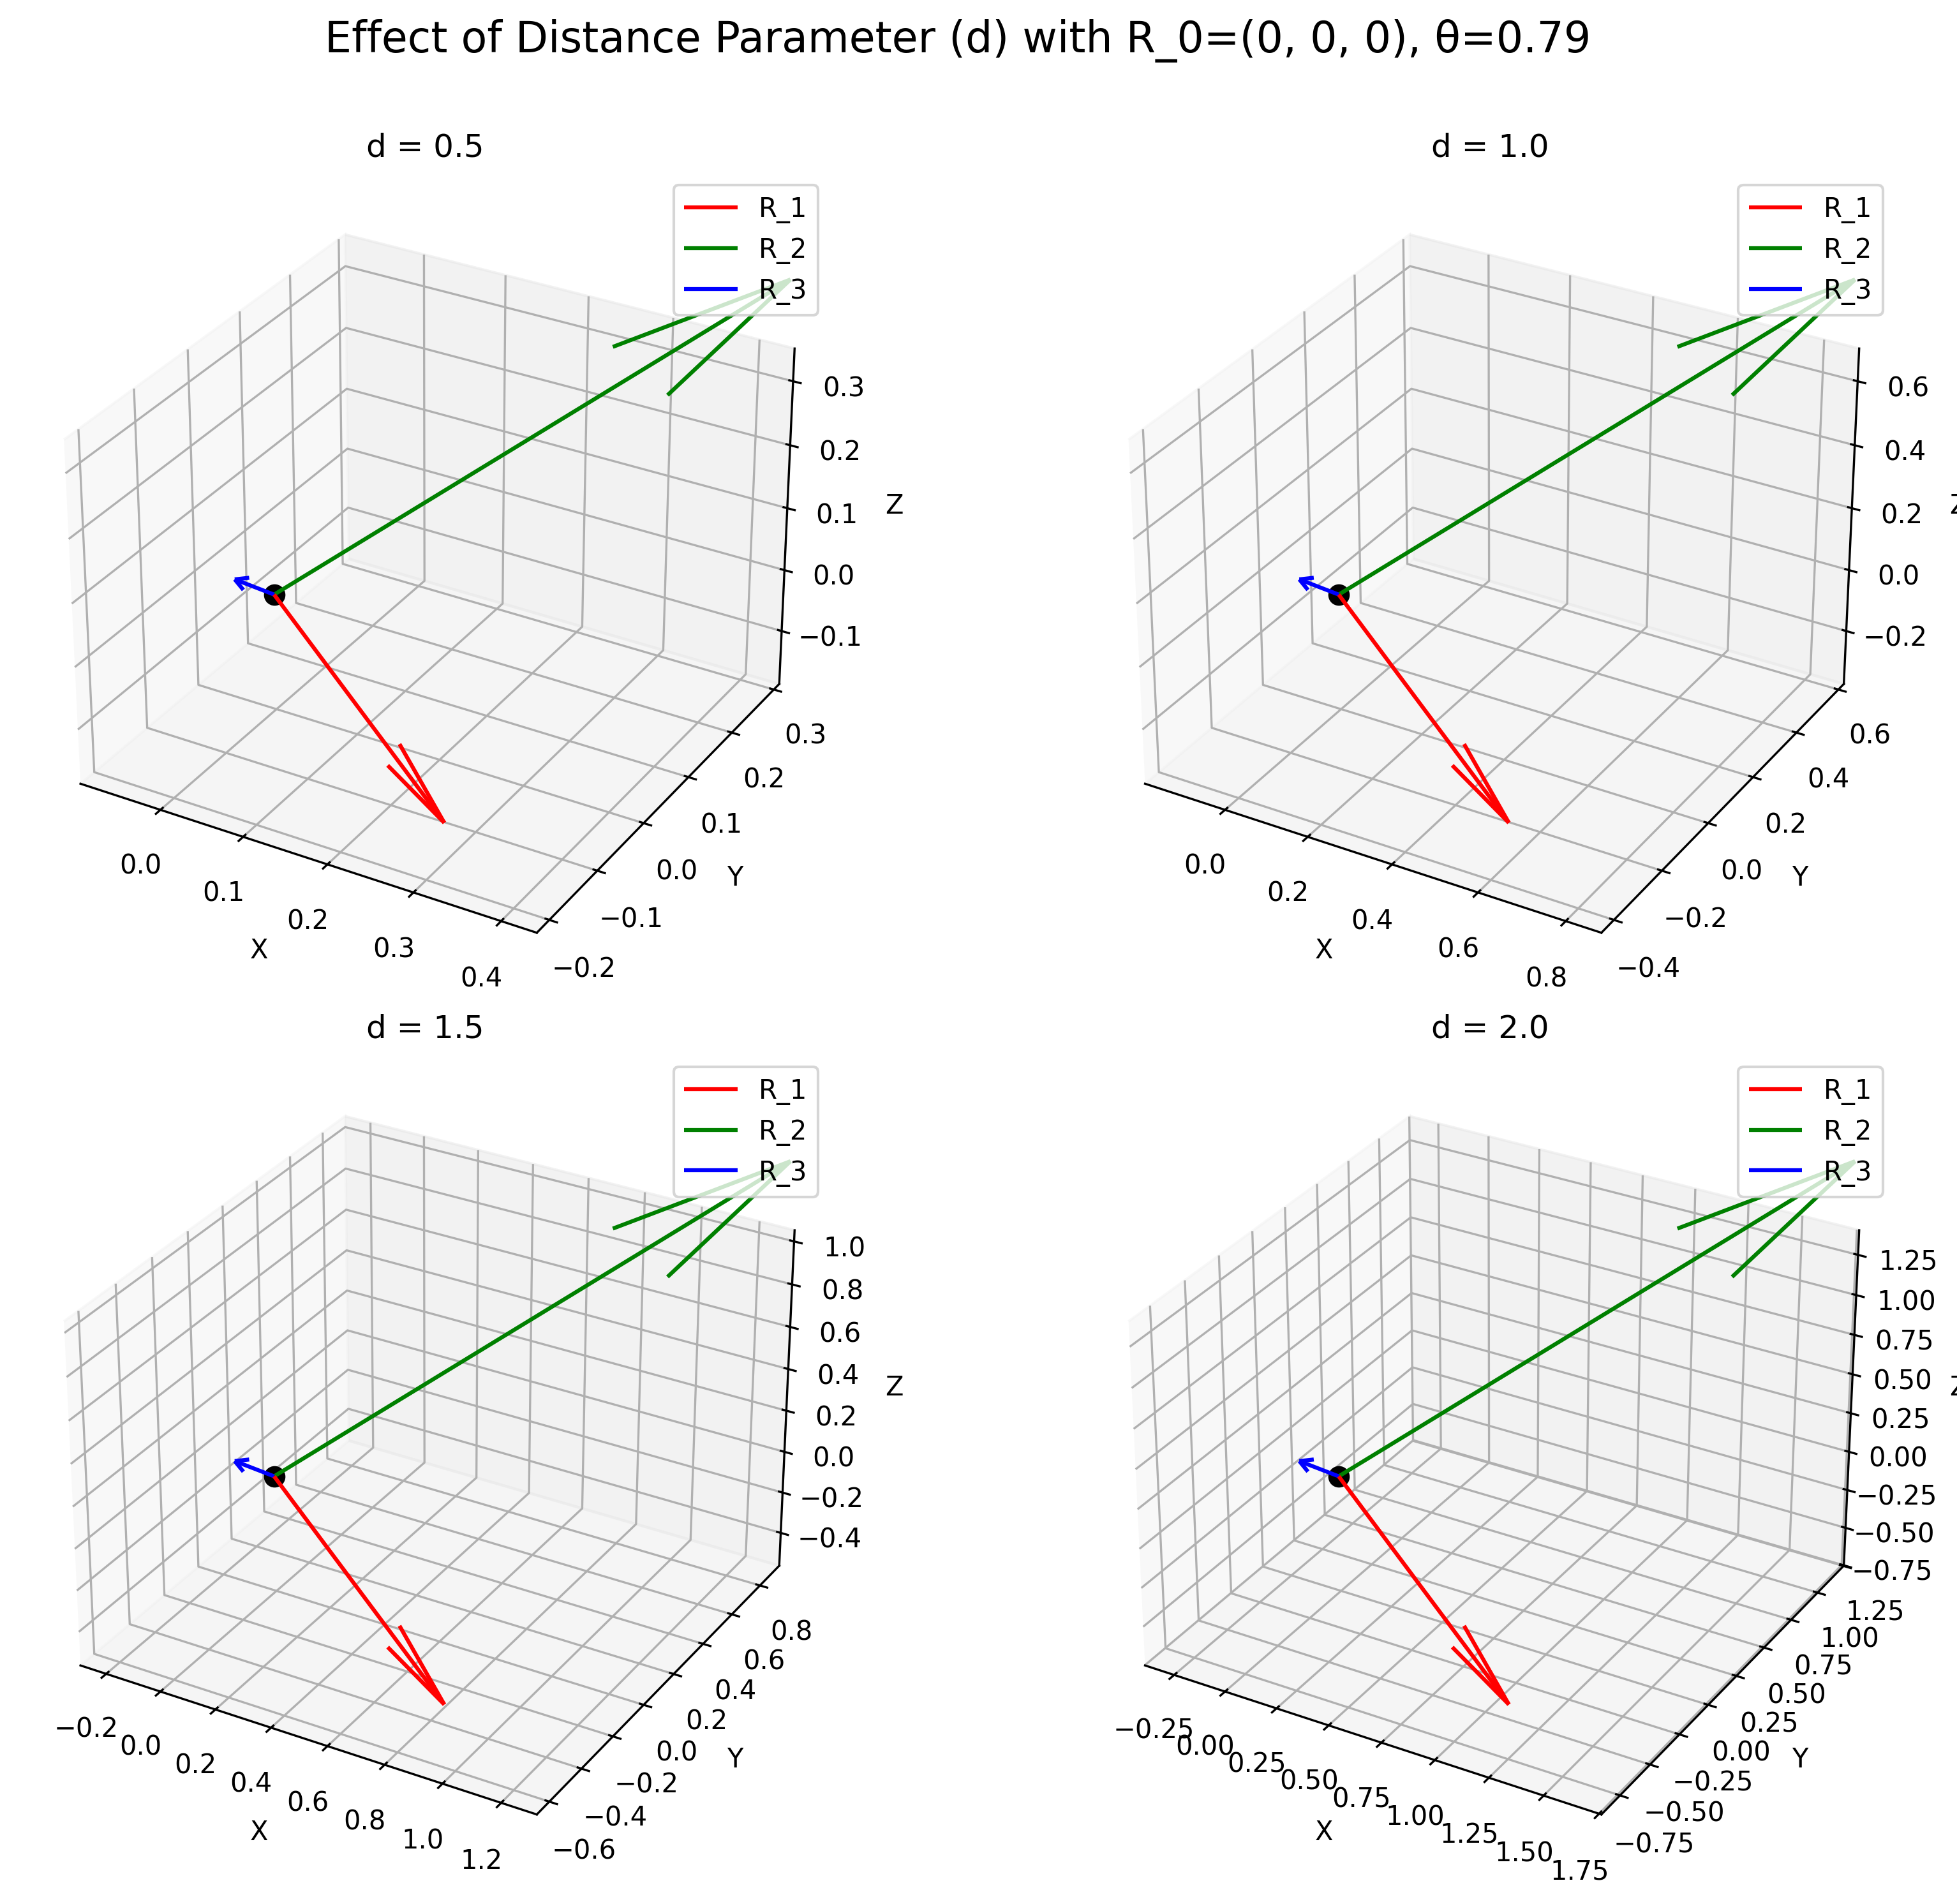
\includegraphics[width=0.9\textwidth]{figures/d_effect_R0_0_0_0.png}
    \caption{Effect of distance parameter on vector visualization with origin at $(0,0,0)$}
    \label{fig:example_distance_effect_default}
\end{figure}

\begin{figure}[H]
    \centering
    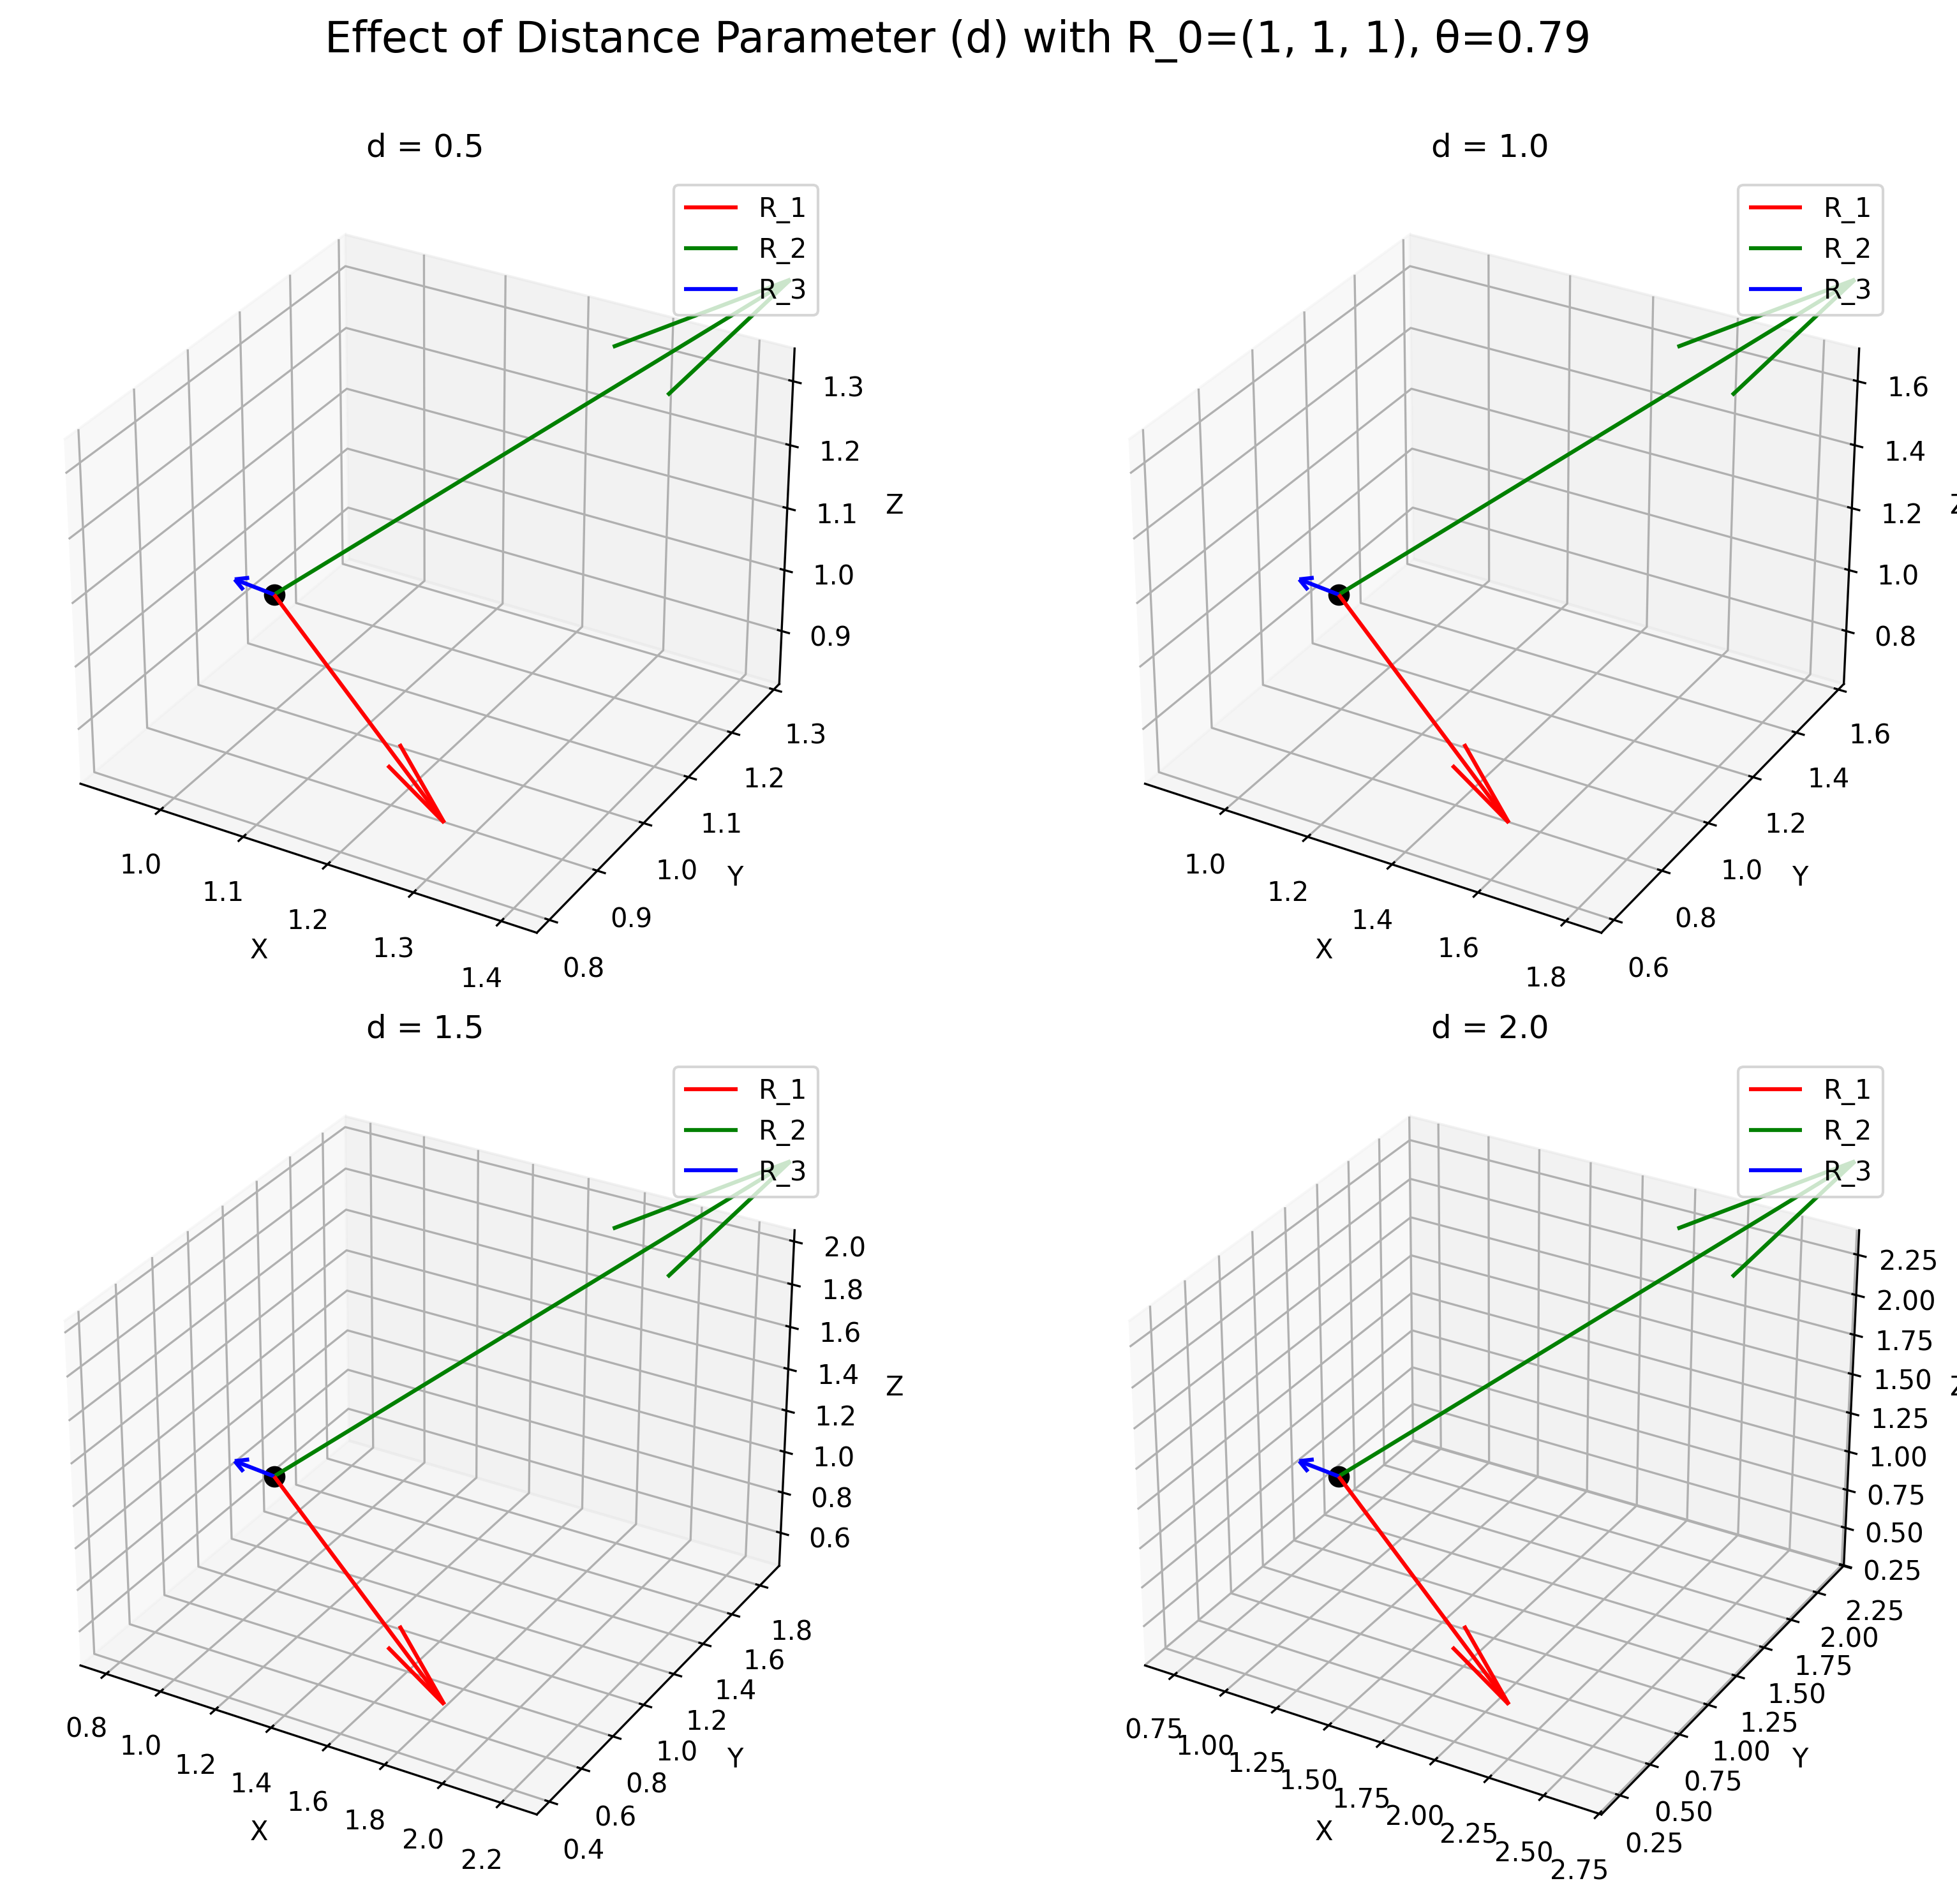
\includegraphics[width=0.9\textwidth]{figures/d_effect_R0_1_1_1.png}
    \caption{Effect of distance parameter on vector visualization with origin at $(1,1,1)$}
    \label{fig:example_distance_effect_custom1}
\end{figure}

\begin{figure}[H]
    \centering
    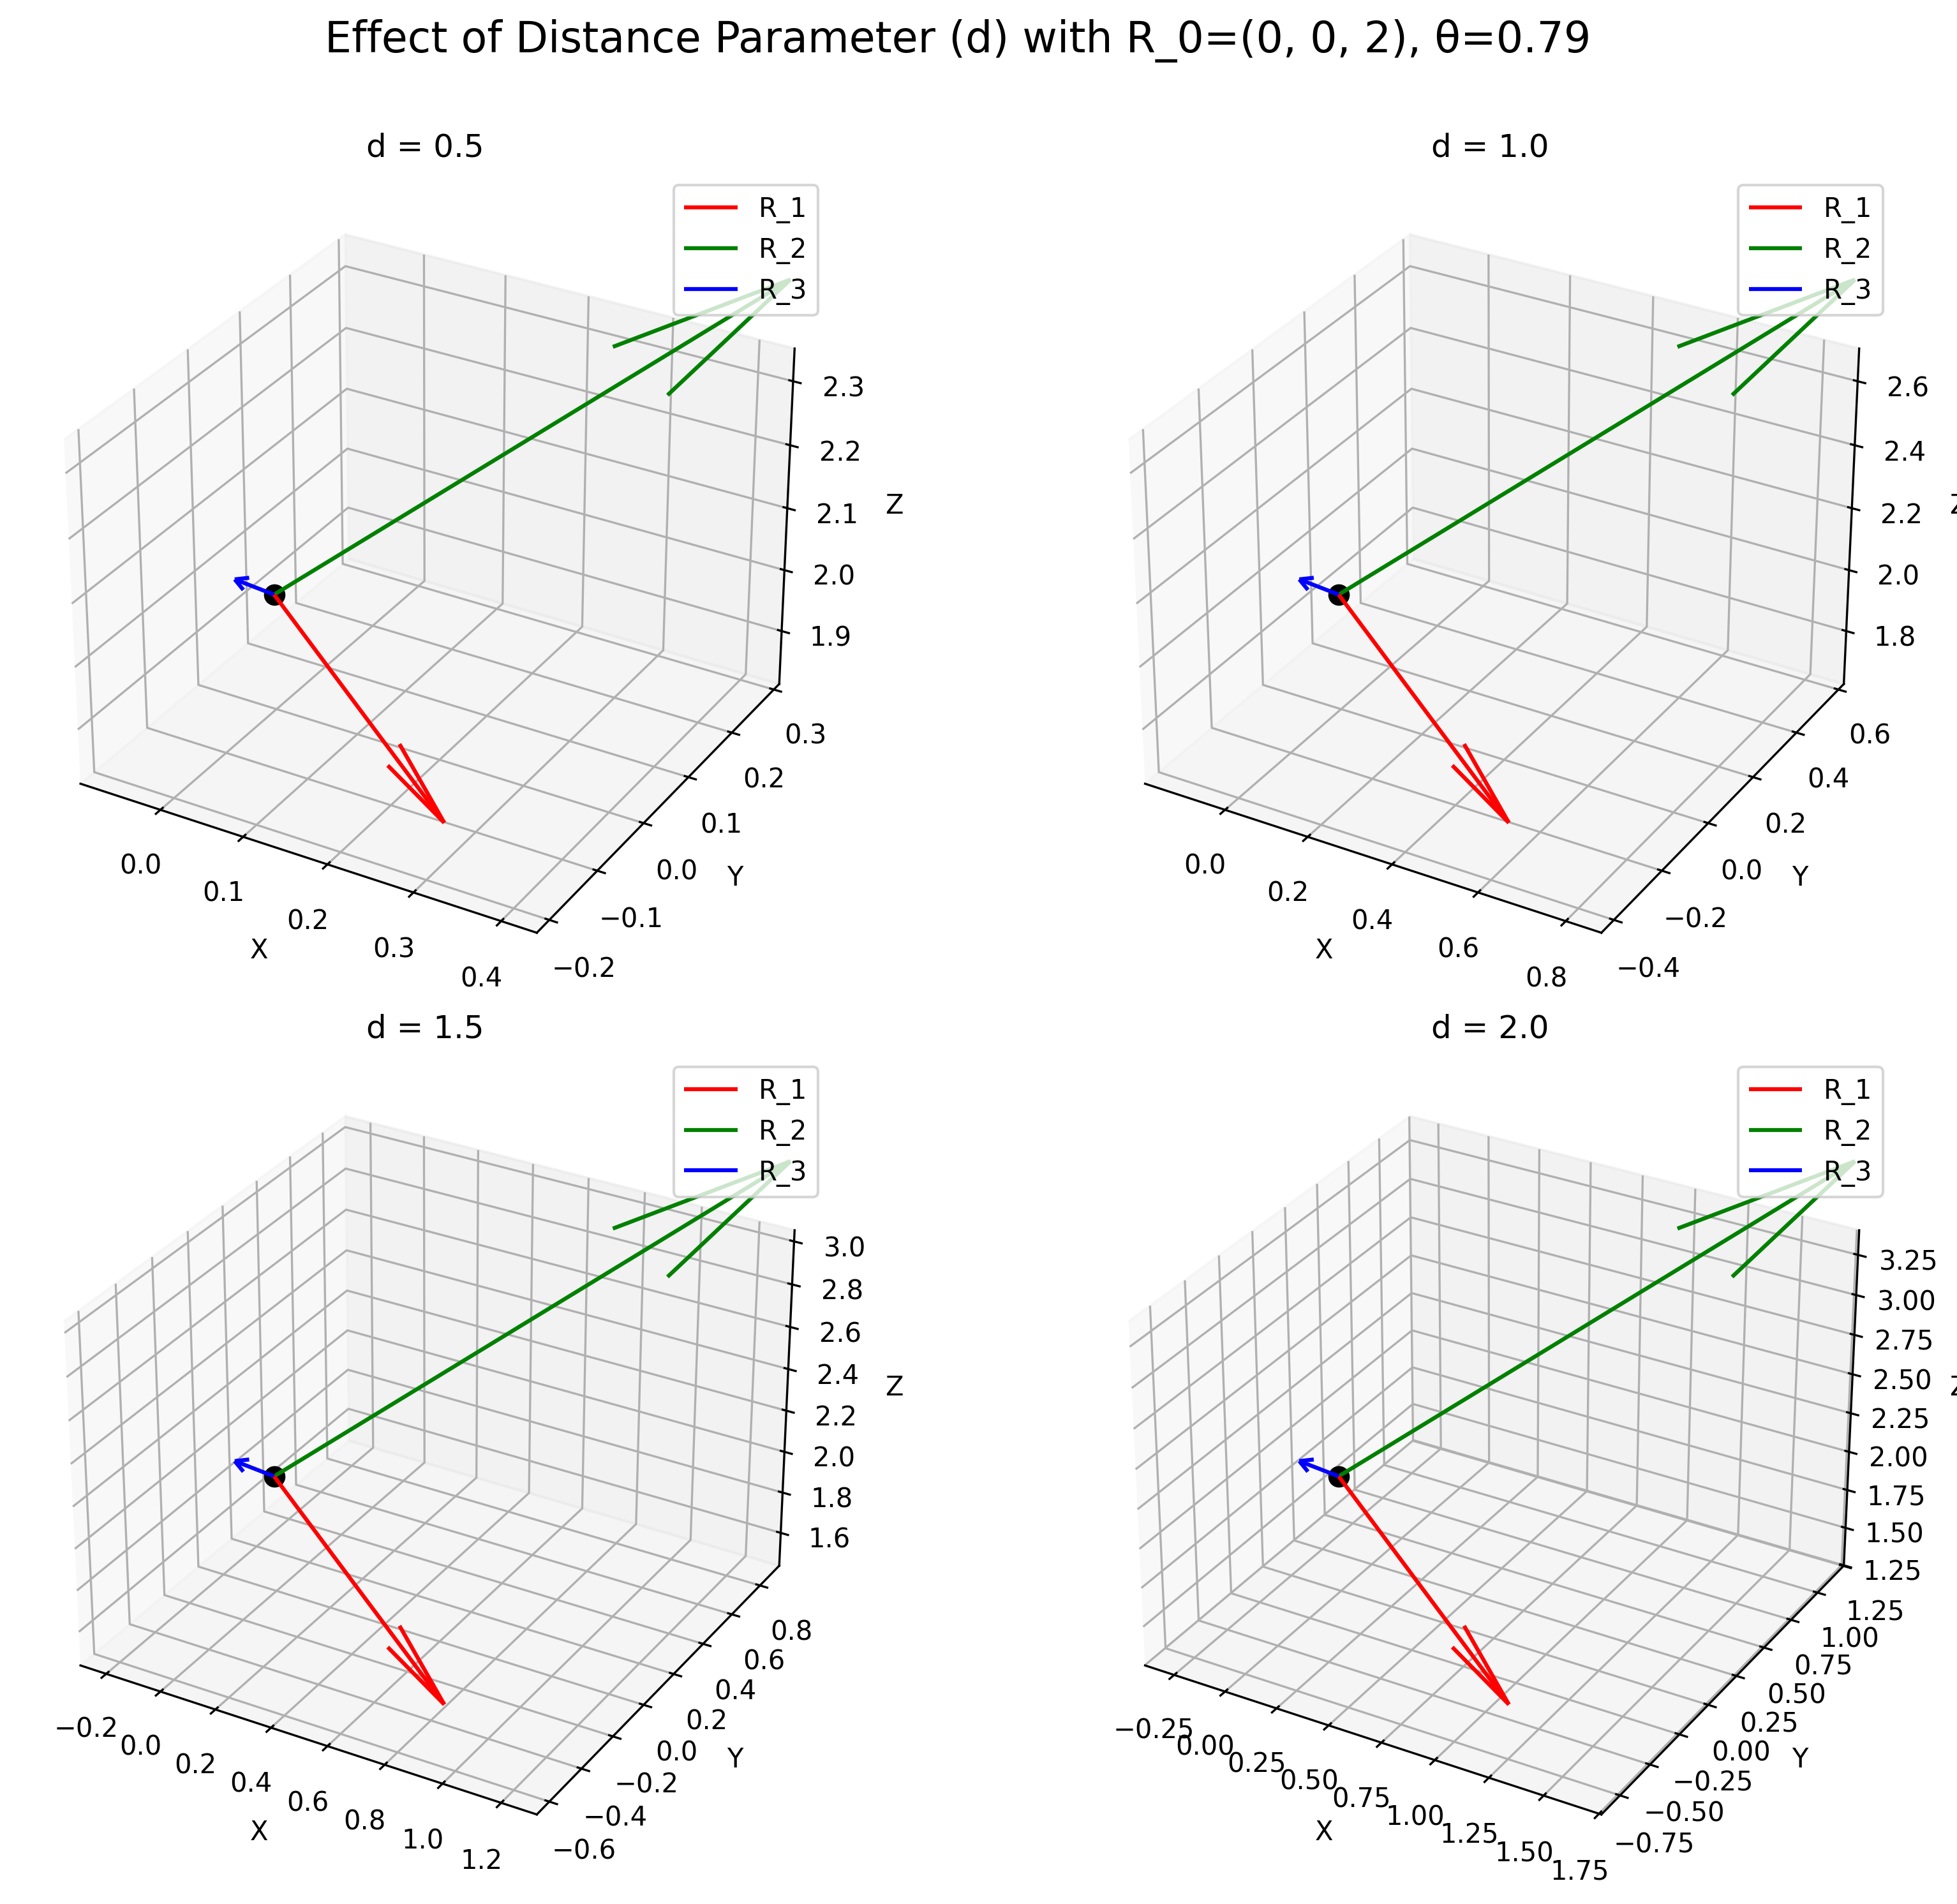
\includegraphics[width=0.9\textwidth]{figures/d_effect_R0_0_0_2.png}
    \caption{Effect of distance parameter on vector visualization with origin at $(0,0,2)$}
    \label{fig:example_distance_effect_custom2}
\end{figure}

\textbf{Effect of Distance Parameter:} The distance parameter $d$ scales the vectors equally, preserving their orthogonality. Increasing $d$ increases the distance of the vectors from the origin, while decreasing $d$ decreases the distance. As shown in the figures above, the effect is consistent across different origin points.

\subsection{Effect of Angle Parameter}

The angle parameter $\theta$ rotates the vectors around the origin, preserving their orthogonality. Different values of $\theta$ result in different orientations of the vectors.

\begin{figure}[H]
    \centering
    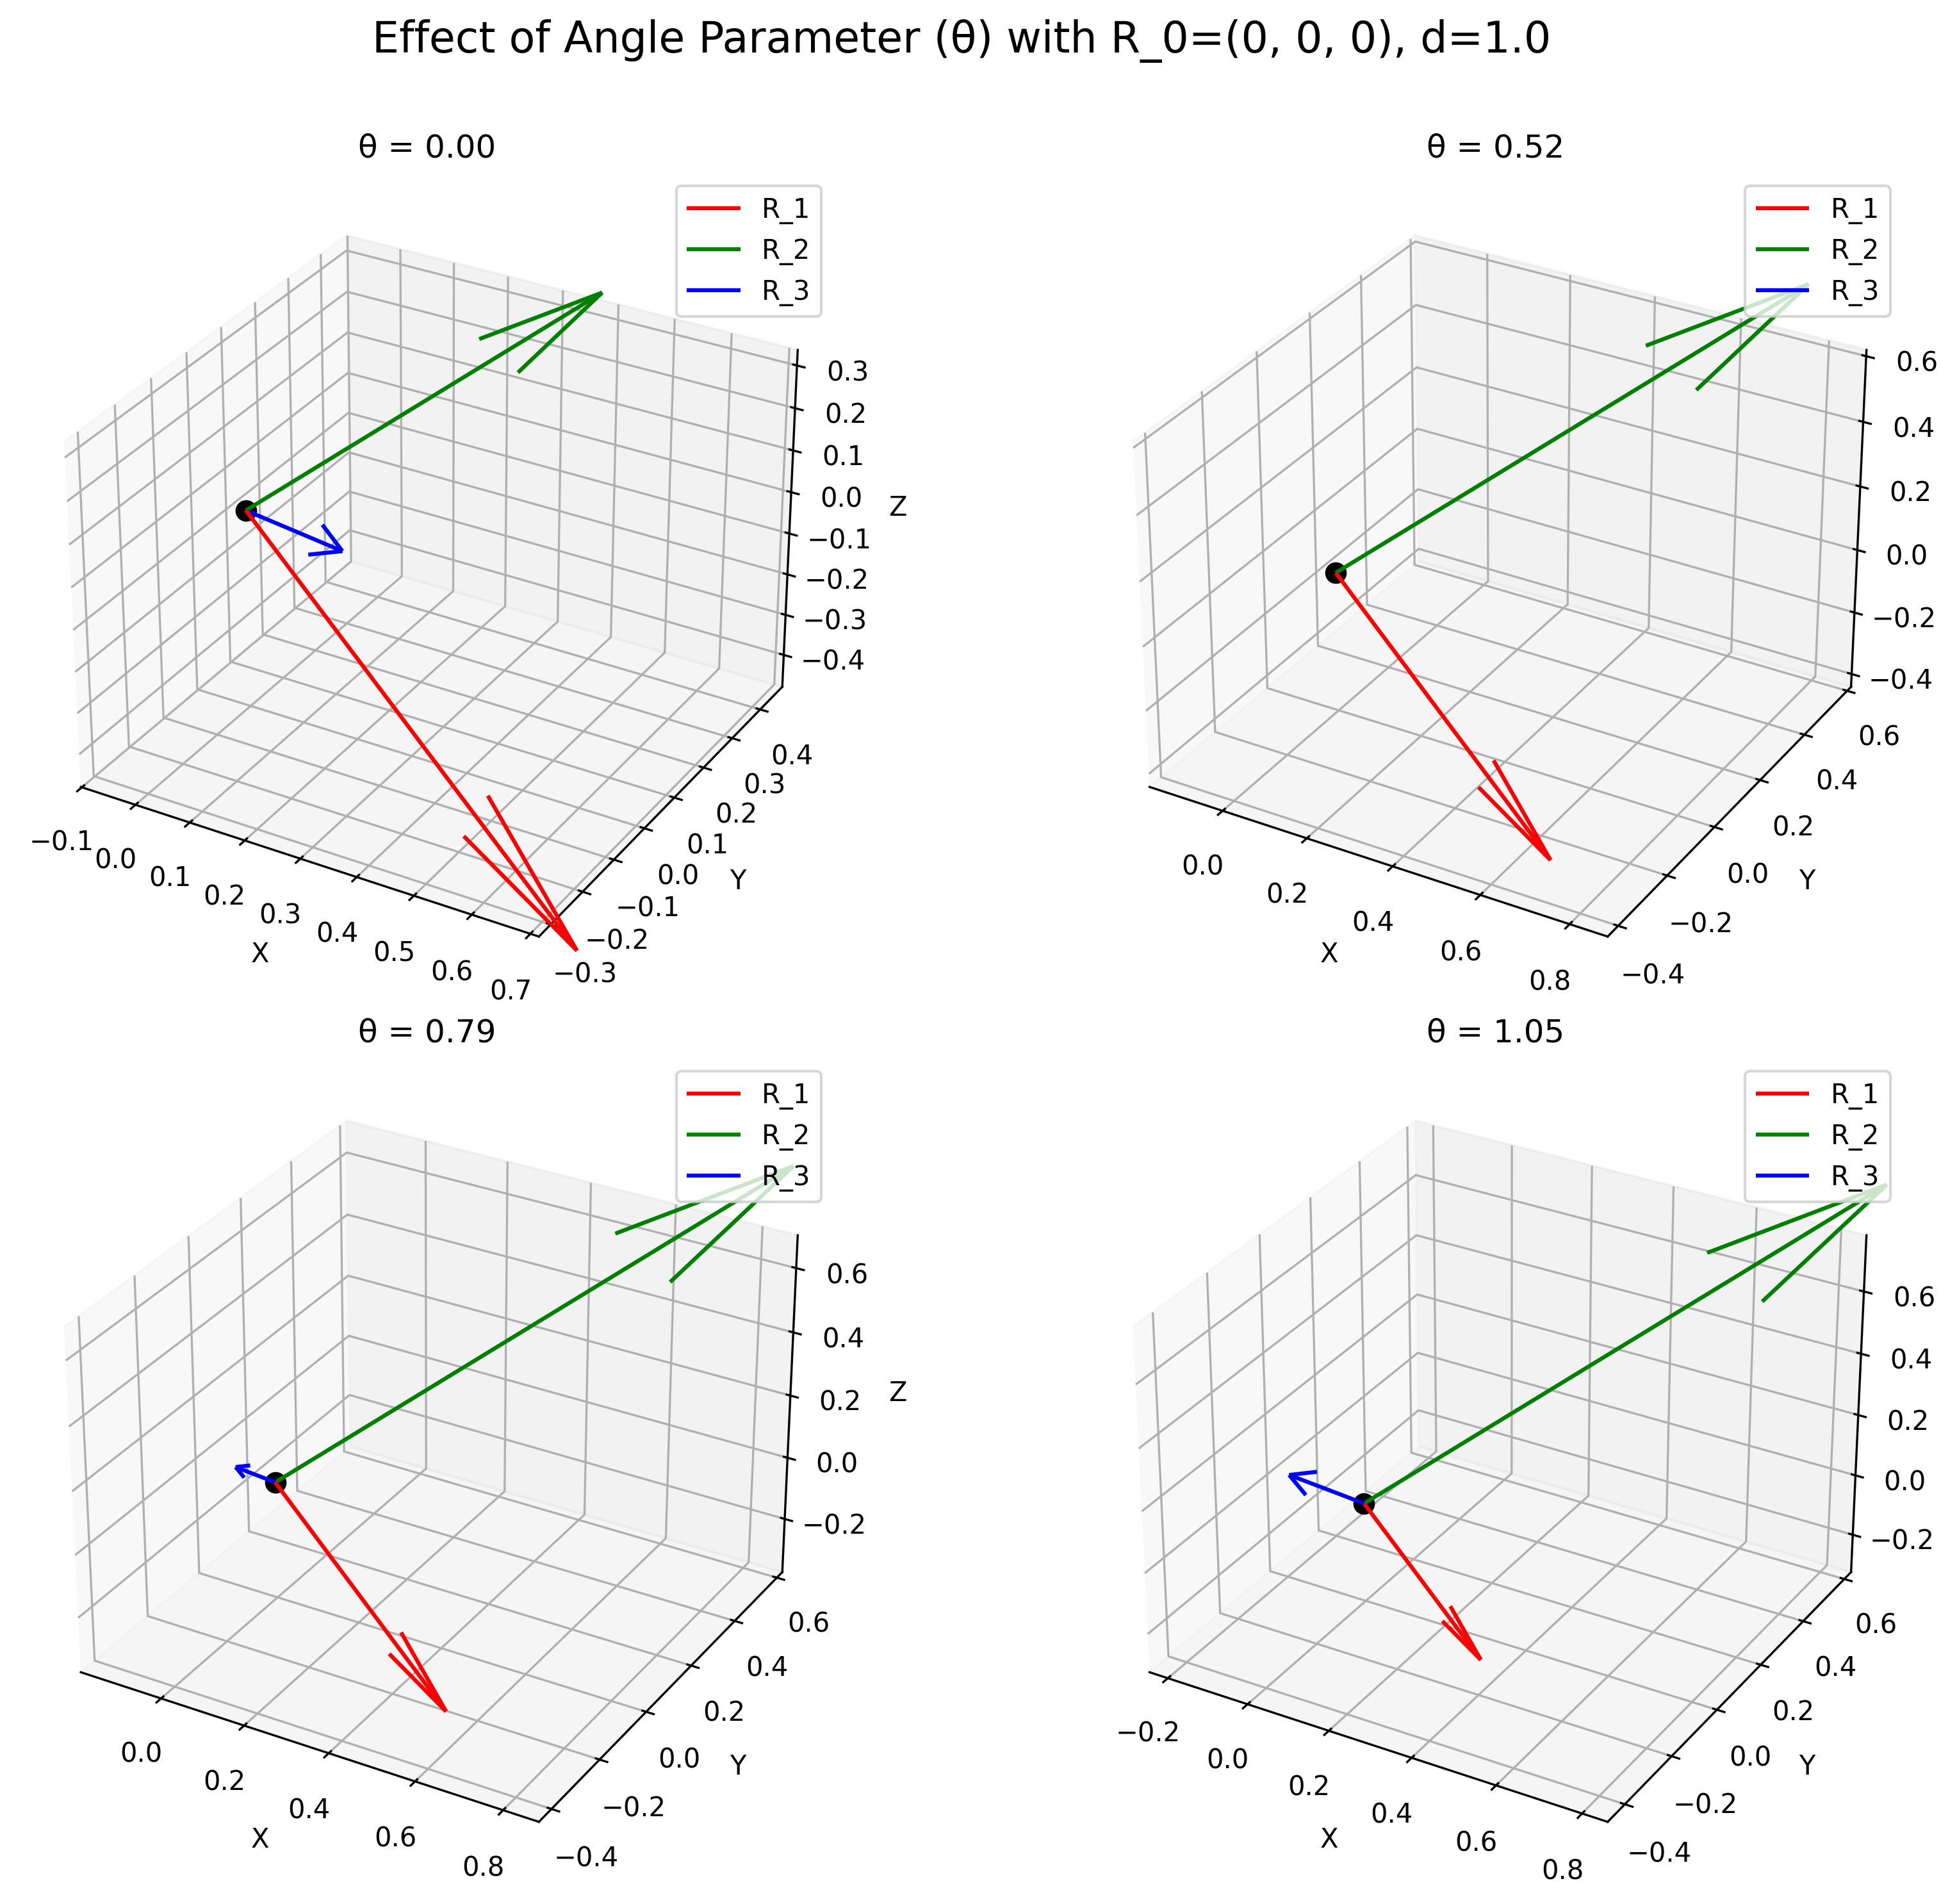
\includegraphics[width=0.9\textwidth]{figures/theta_effect_R0_0_0_0.png}
    \caption{Effect of angle parameter on vector visualization with origin at $(0,0,0)$}
    \label{fig:example_angle_effect_default}
\end{figure}

\begin{figure}[H]
    \centering
    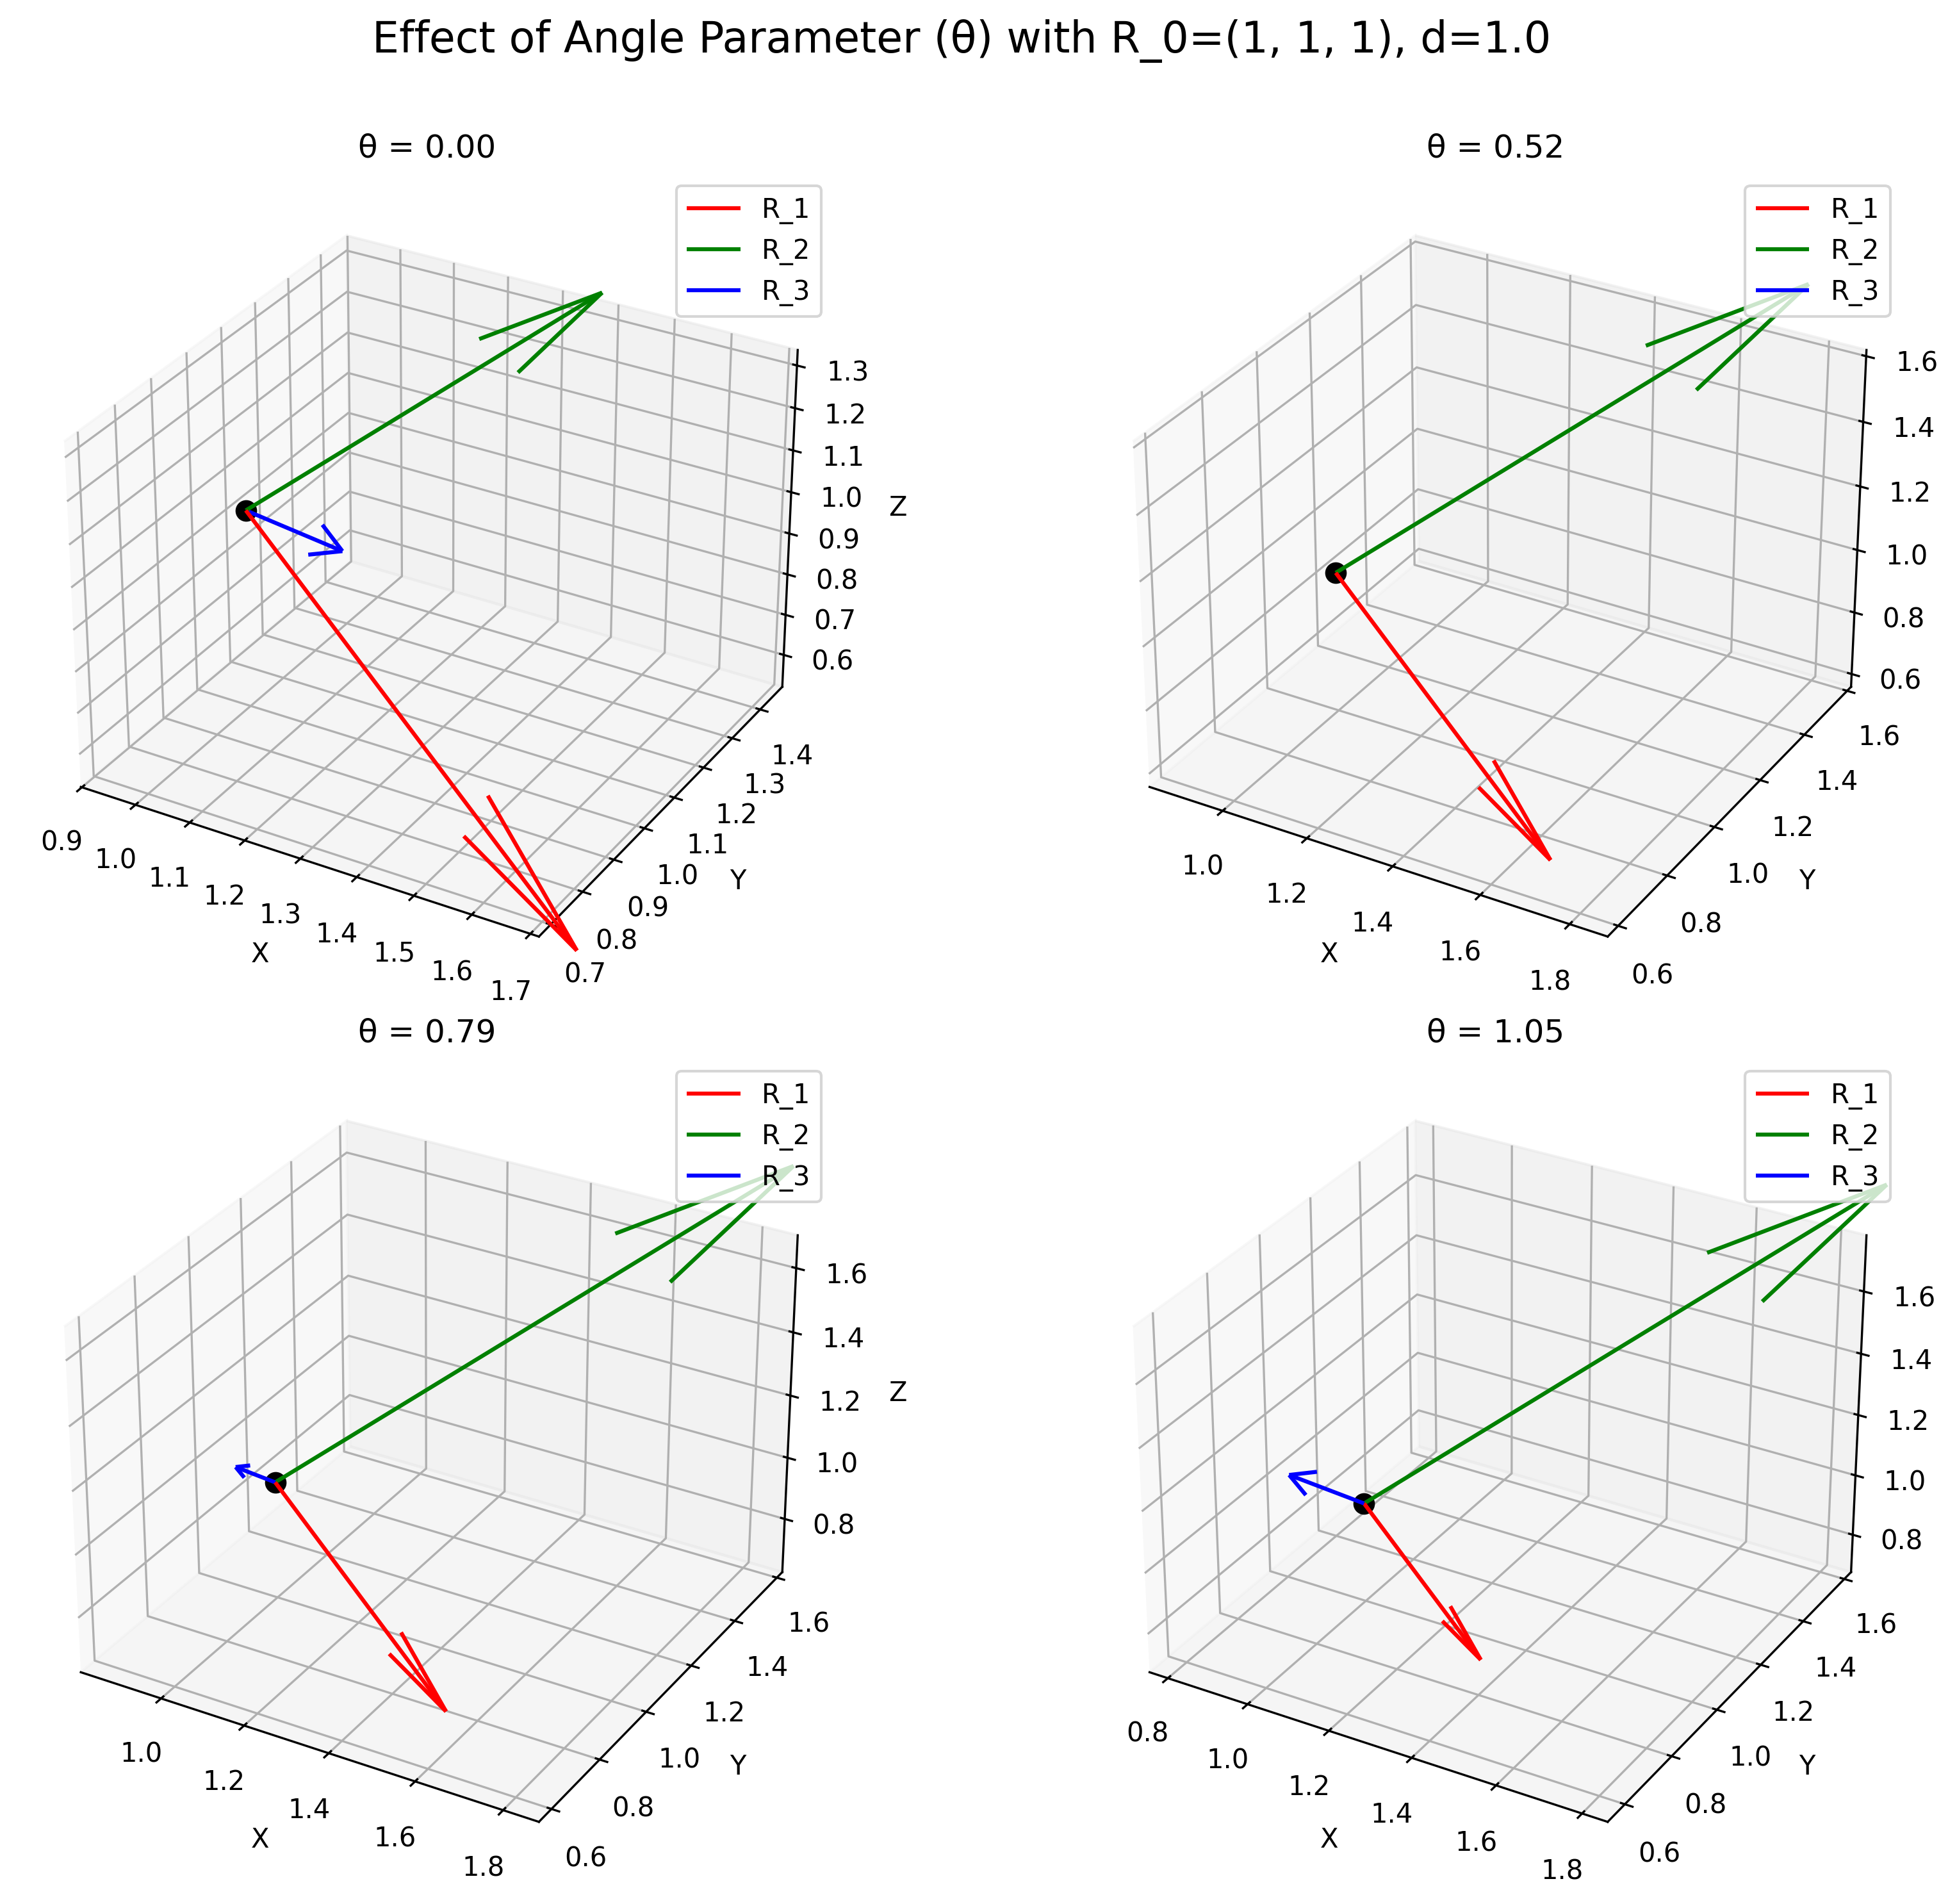
\includegraphics[width=0.9\textwidth]{figures/theta_effect_R0_1_1_1.png}
    \caption{Effect of angle parameter on vector visualization with origin at $(1,1,1)$}
    \label{fig:example_angle_effect_custom1}
\end{figure}

\begin{figure}[H]
    \centering
    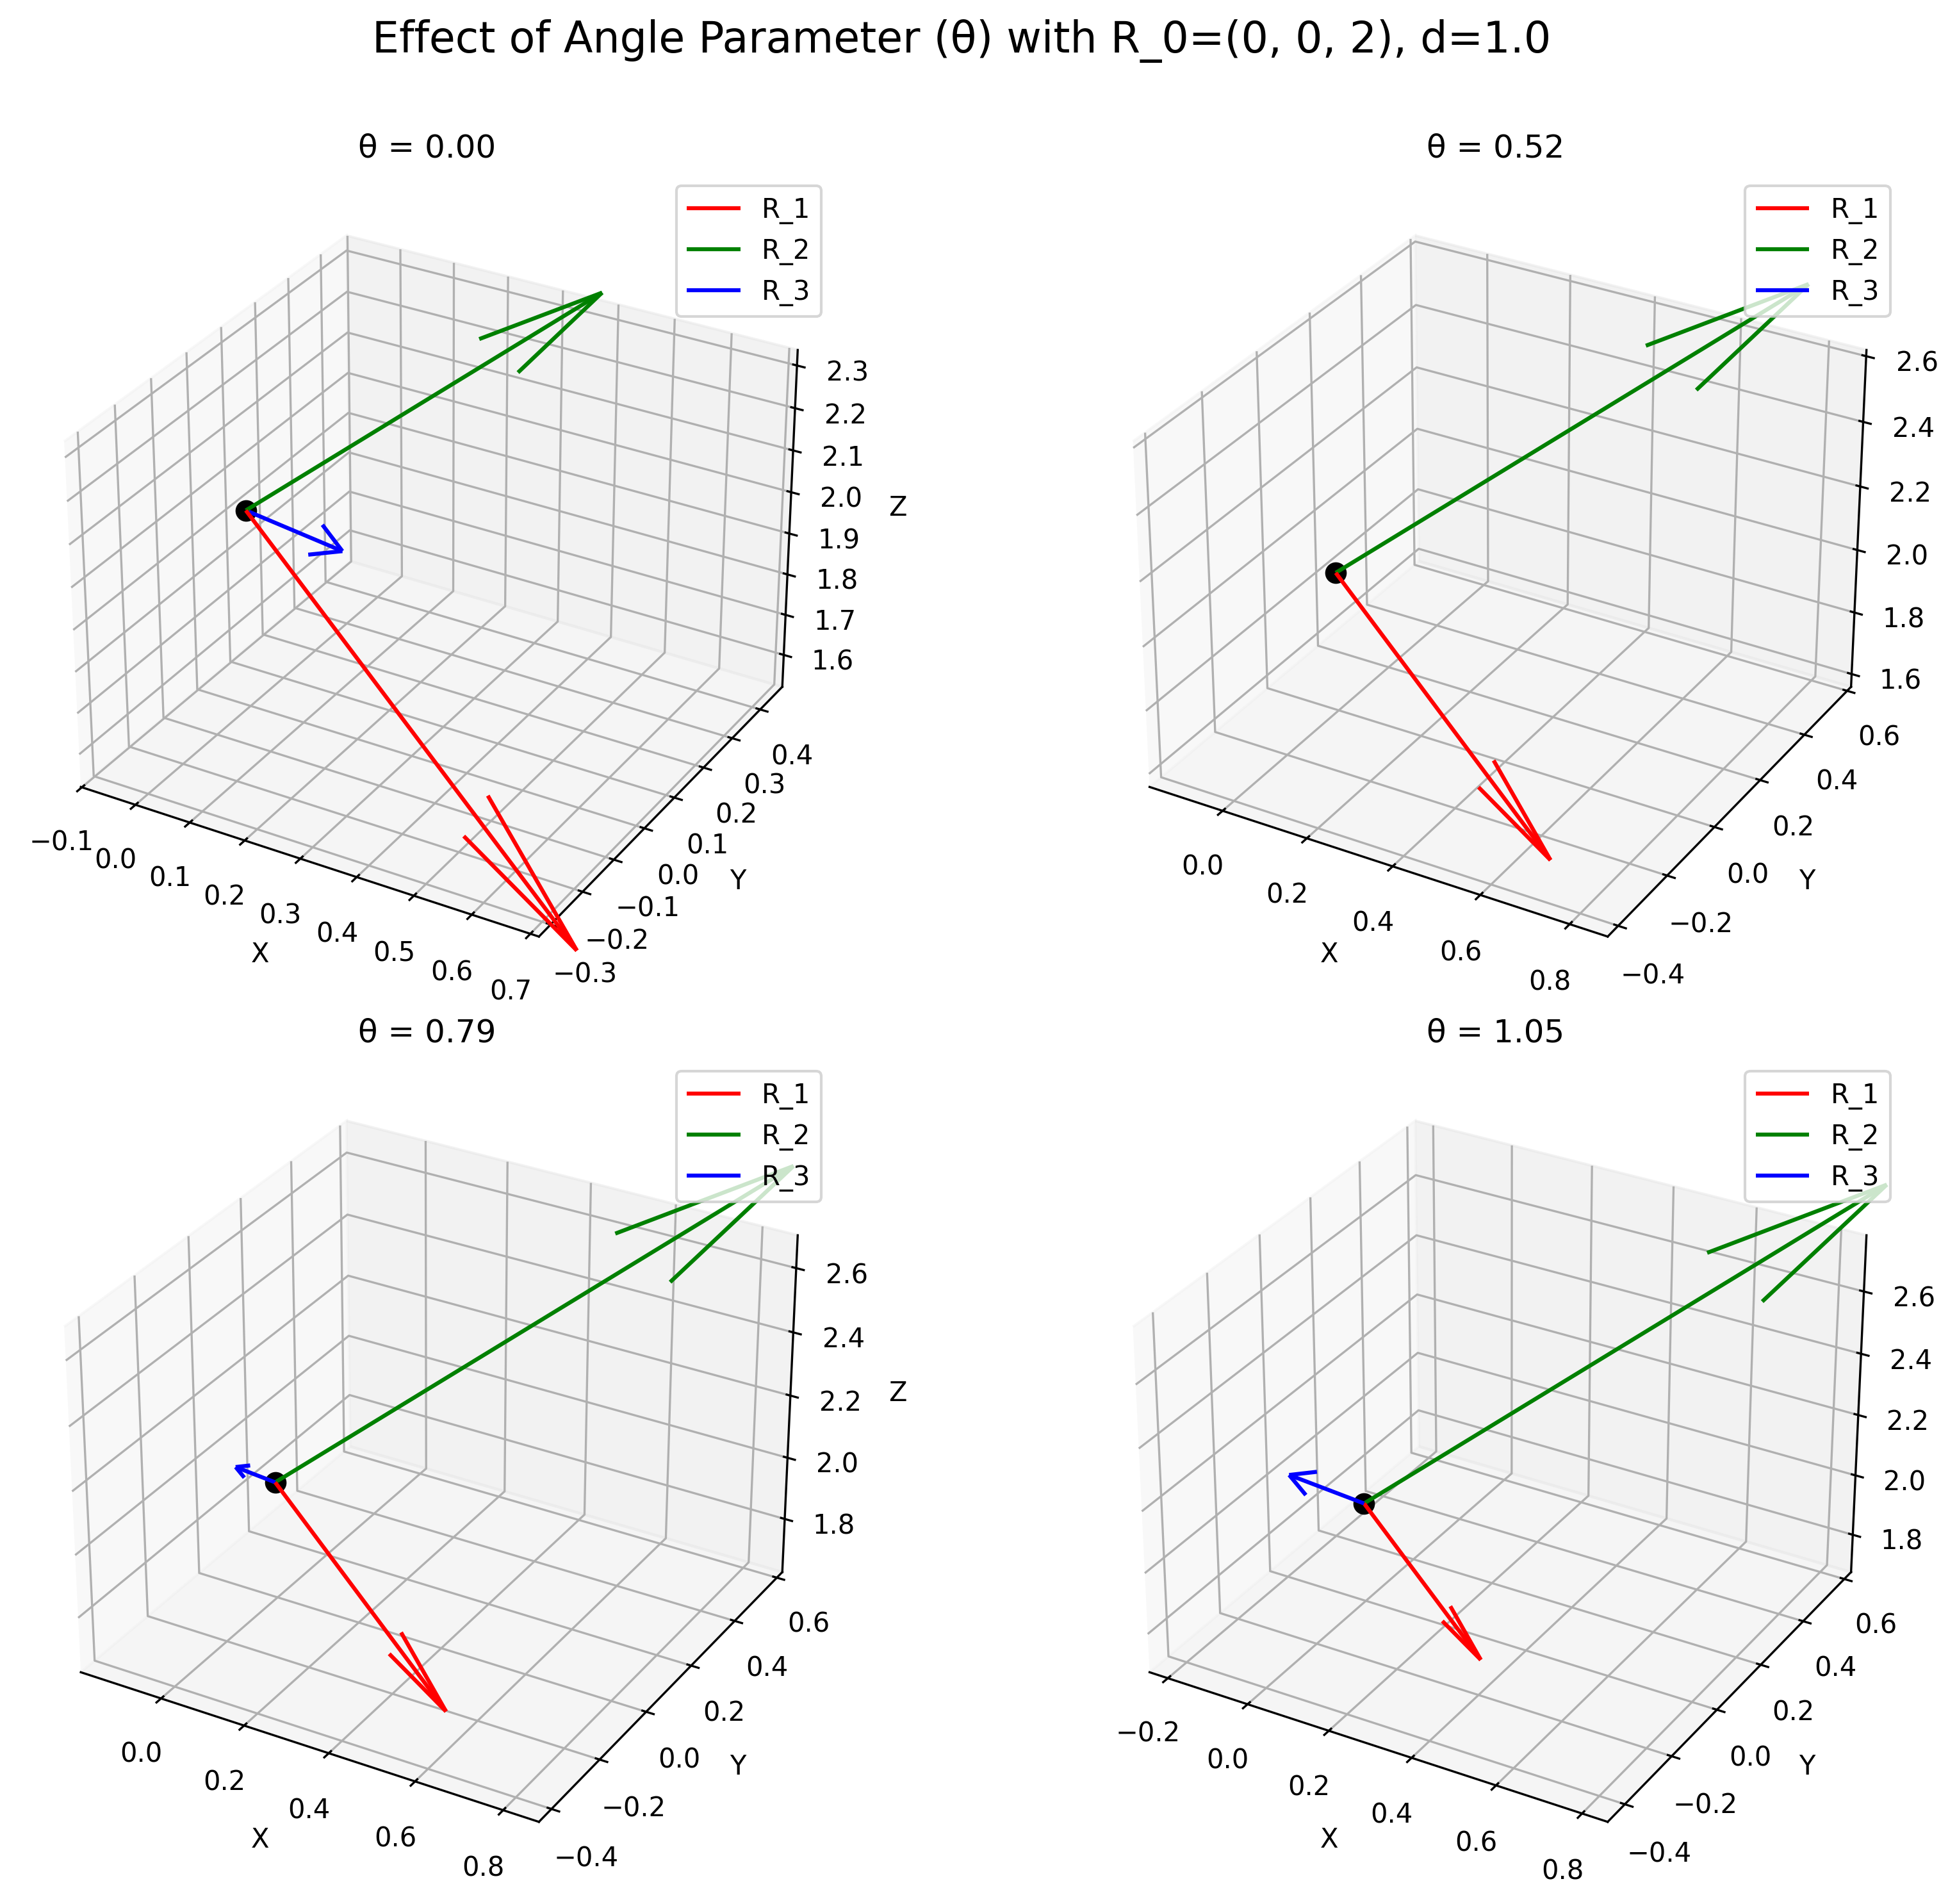
\includegraphics[width=0.9\textwidth]{figures/theta_effect_R0_0_0_2.png}
    \caption{Effect of angle parameter on vector visualization with origin at $(0,0,2)$}
    \label{fig:example_angle_effect_custom2}
\end{figure}

\textbf{Effect of Angle Parameter:} The angle parameter $\theta$ rotates the vectors around the origin, preserving their orthogonality. Different values of $\theta$ result in different orientations of the vectors. As shown in the figures above, the effect is consistent across different origin points, with the rotation occurring relative to the specified origin.

\subsection{Effect of Origin}

The origin parameter $\vec{R}_0$ shifts the entire vector system, preserving the orthogonality of the displacement vectors. Different origin points result in different positions of the vectors in space.

\subsubsection{3D Visualizations}

\begin{figure}[H]
    \centering
    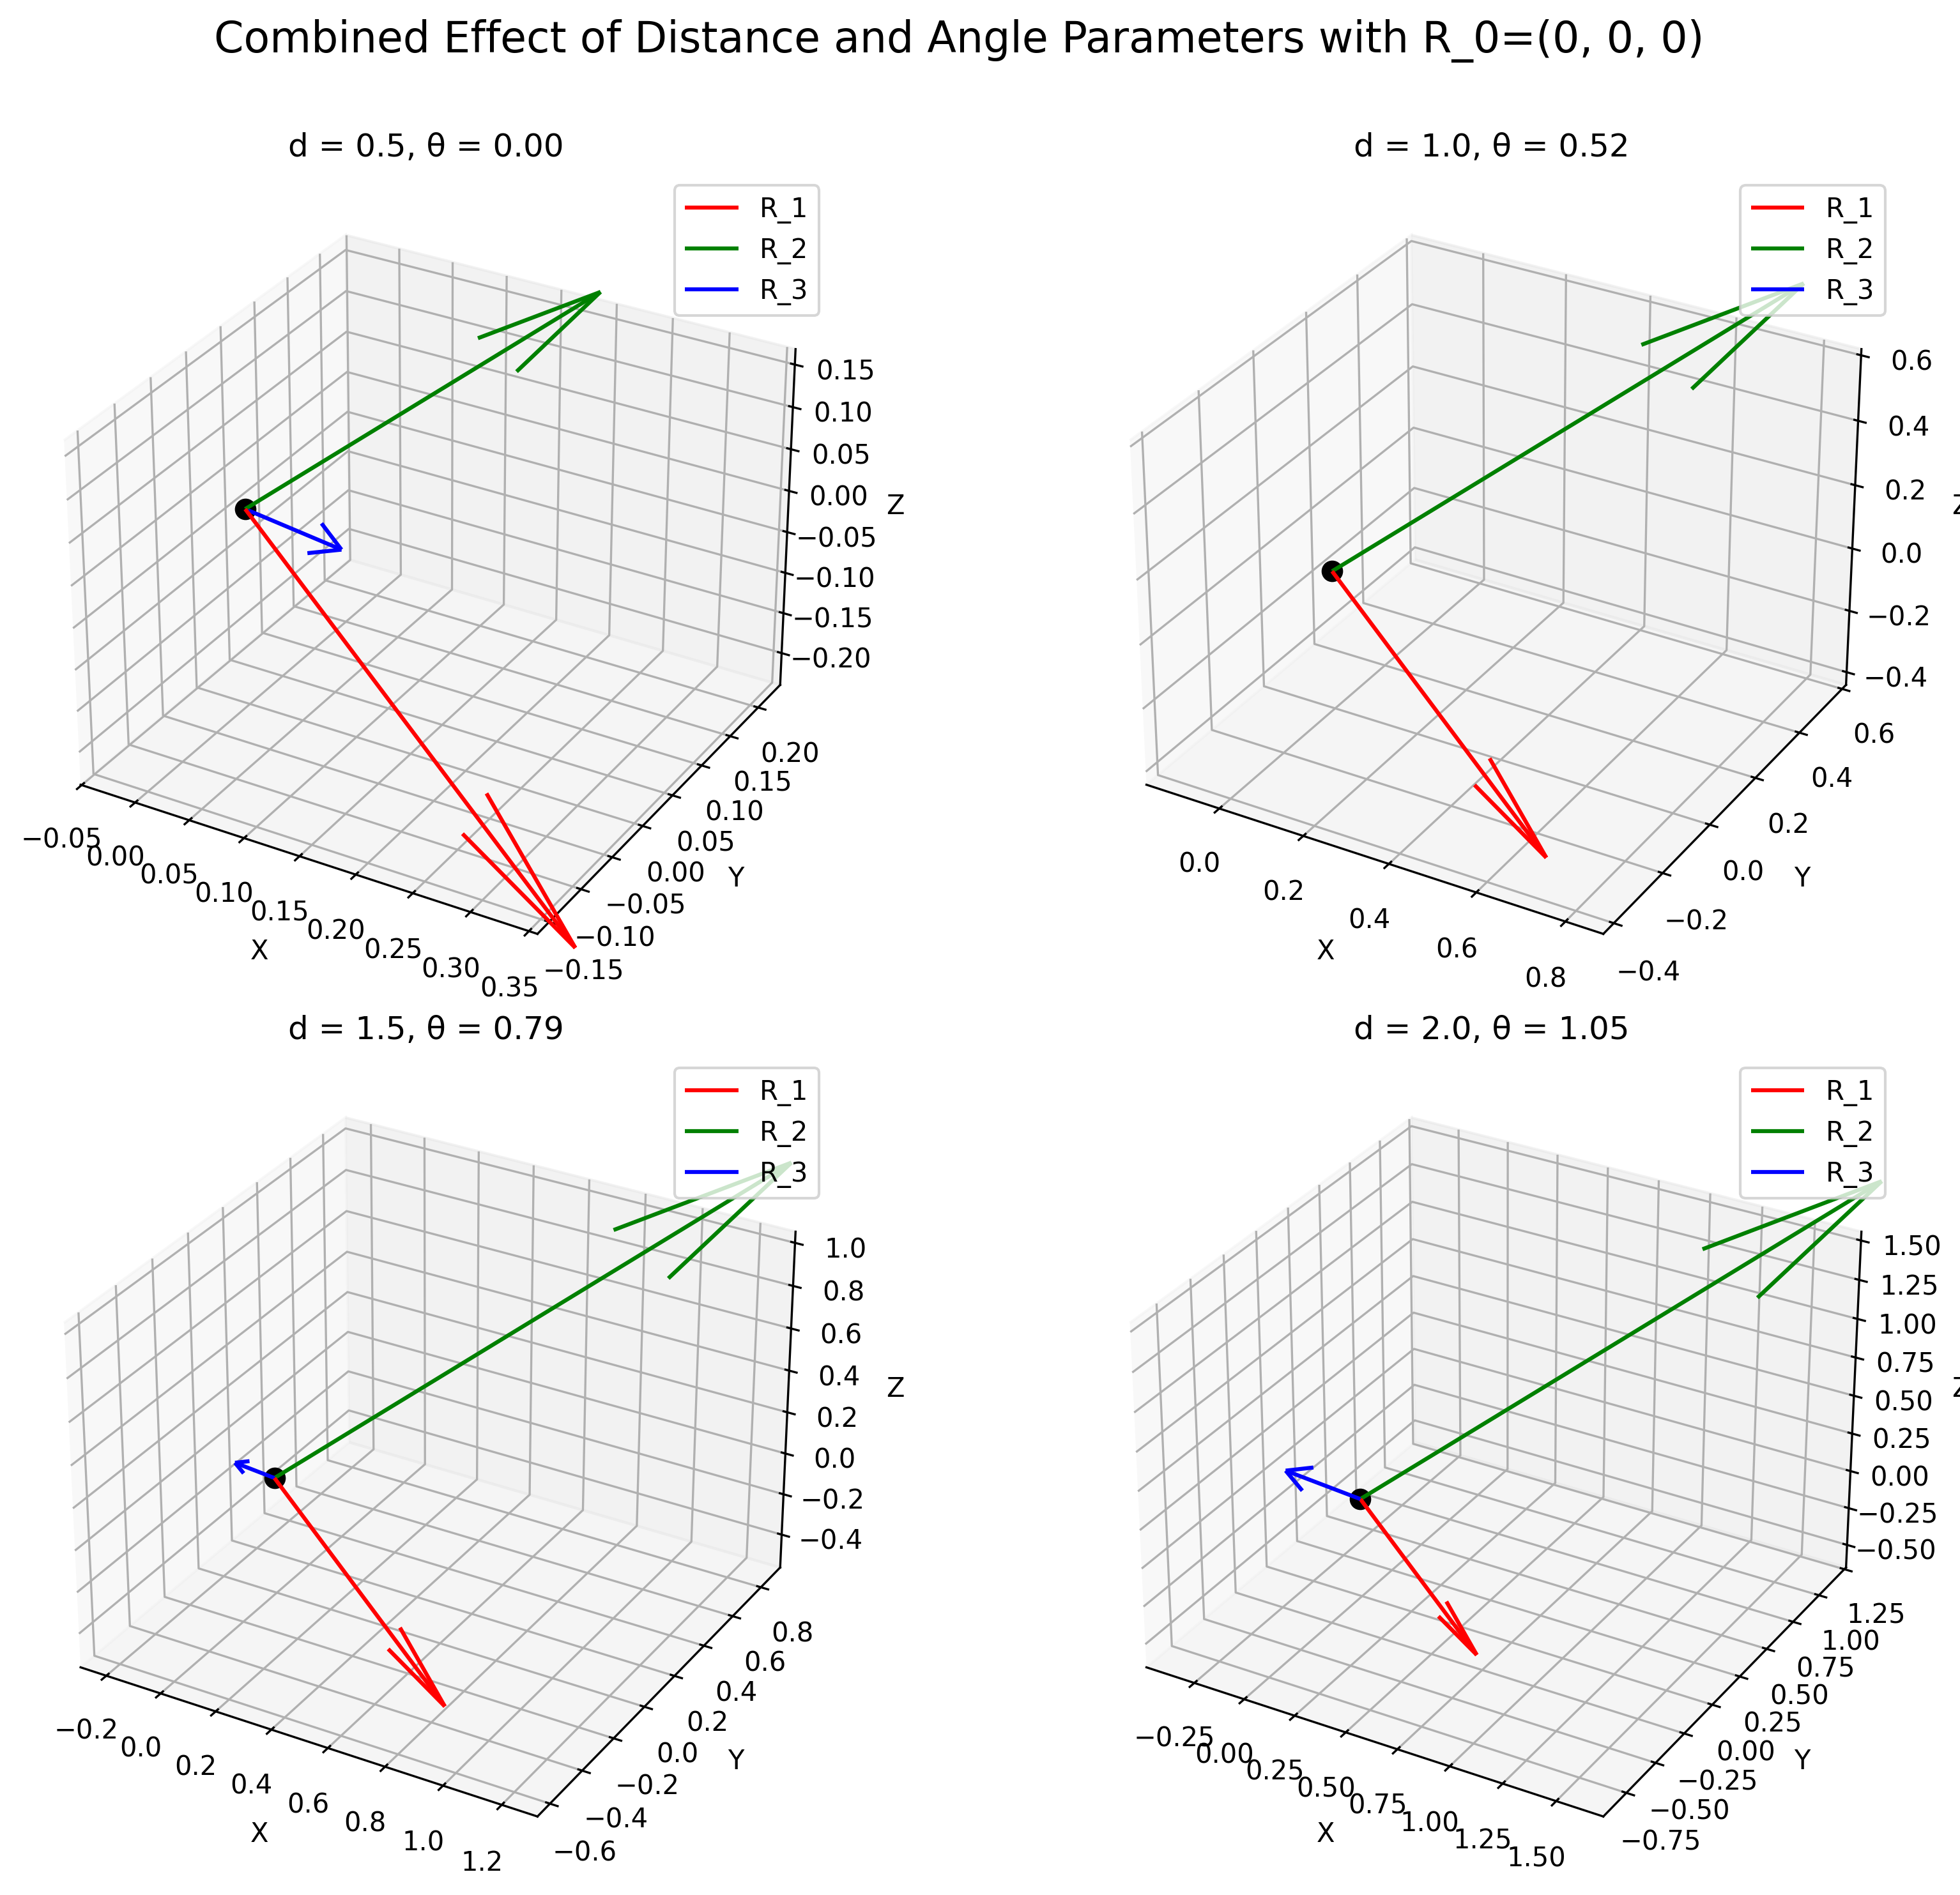
\includegraphics[width=0.9\textwidth]{figures/combined_effect_R0_0_0_0.png}
    \caption{Combined effect of distance and angle parameters with origin at $(0,0,0)$}
    \label{fig:example_combined_effect_default}
\end{figure}

\begin{figure}[H]
    \centering
    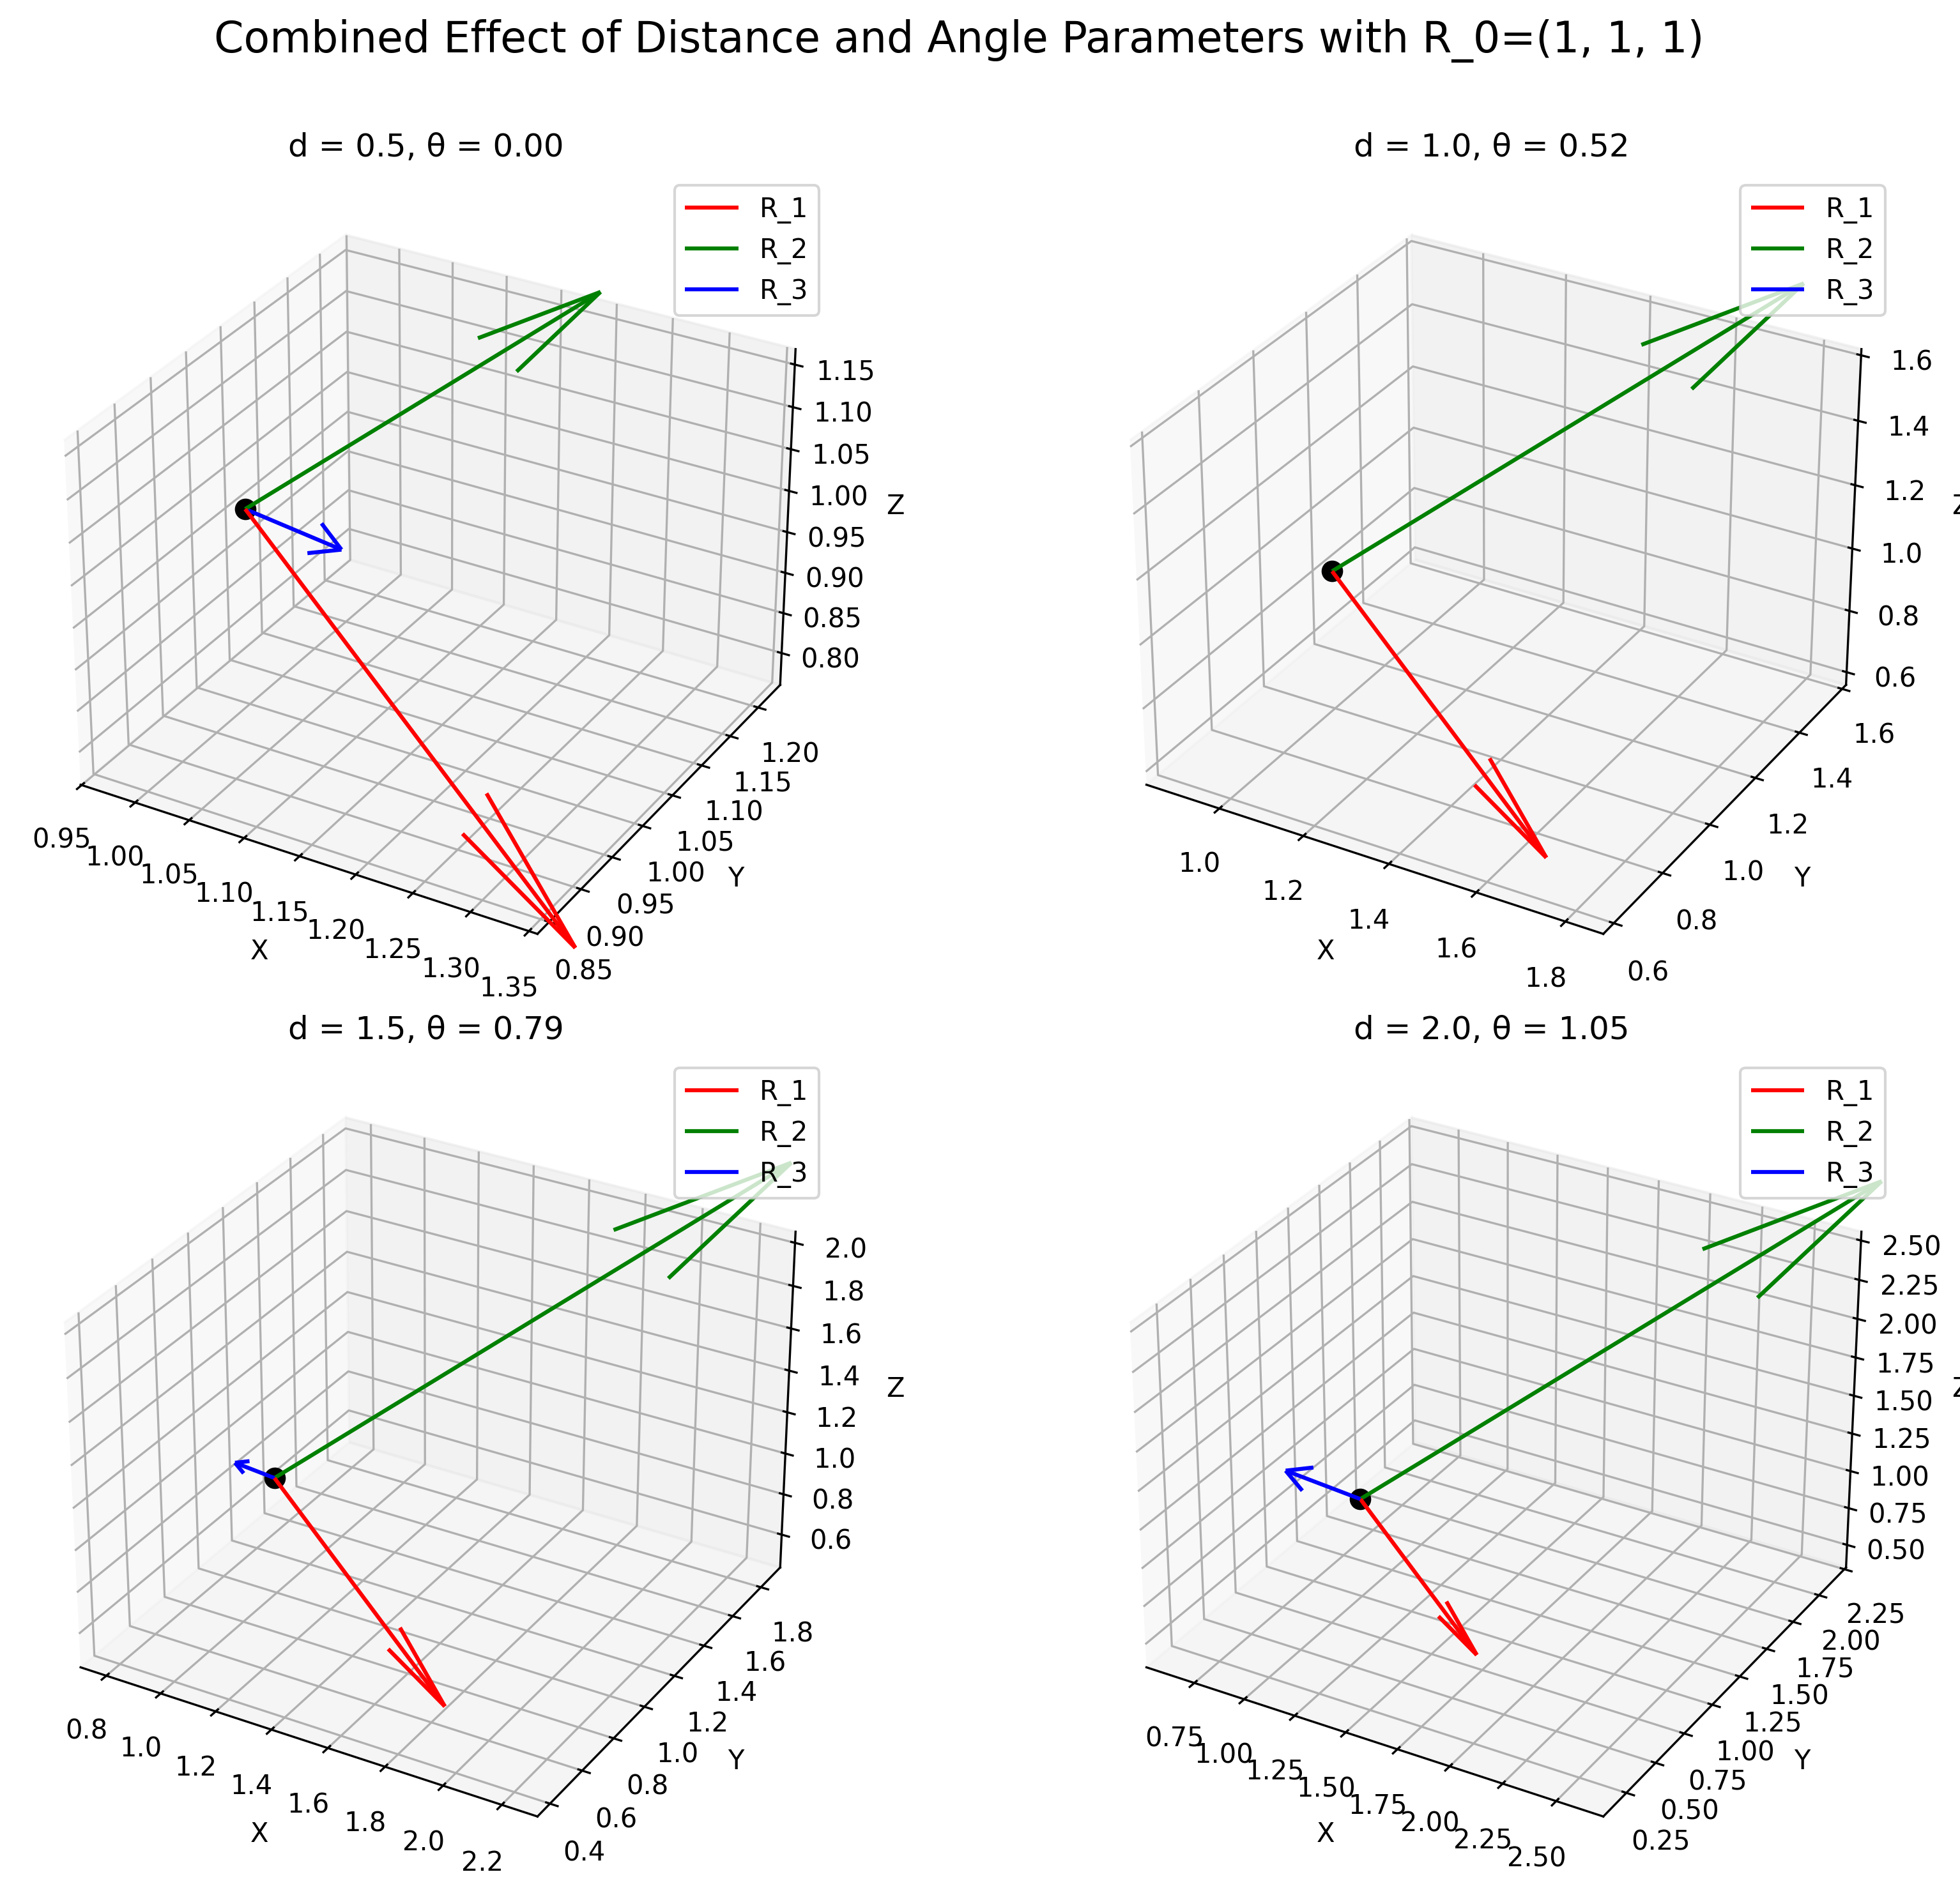
\includegraphics[width=0.9\textwidth]{figures/combined_effect_R0_1_1_1.png}
    \caption{Combined effect of distance and angle parameters with origin at $(1,1,1)$}
    \label{fig:example_combined_effect_custom1}
\end{figure}

\begin{figure}[H]
    \centering
    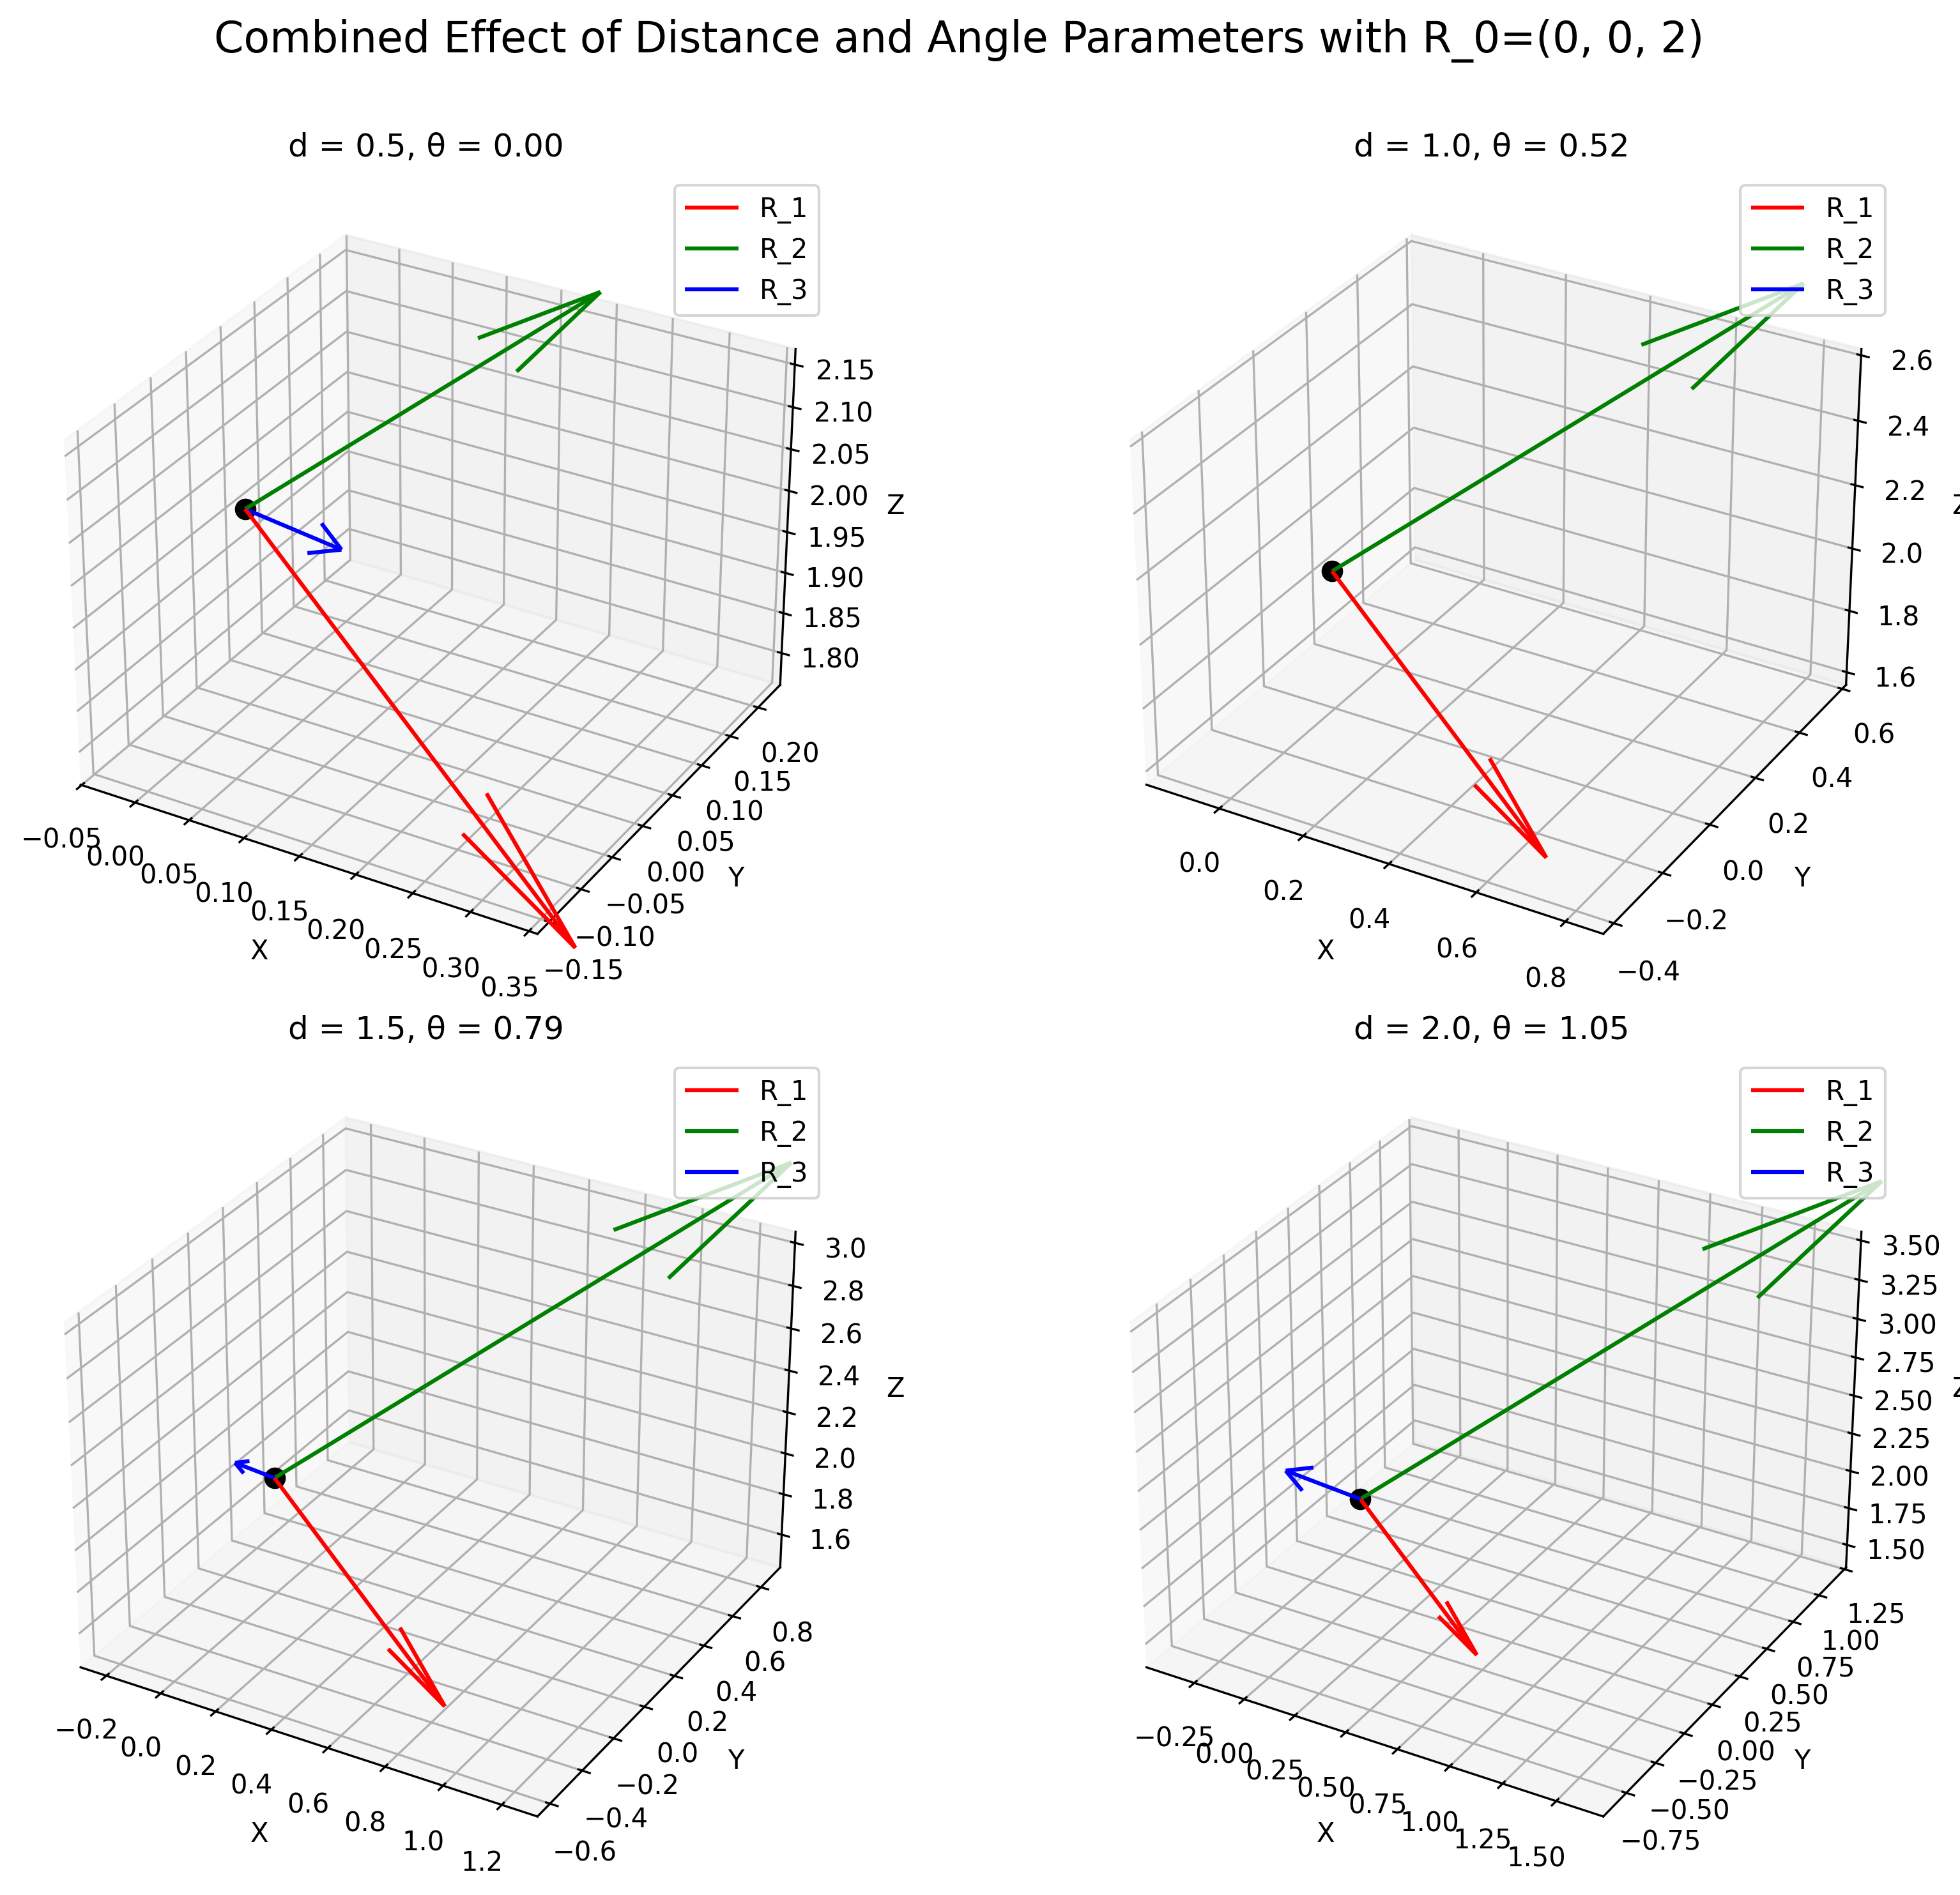
\includegraphics[width=0.9\textwidth]{figures/combined_effect_R0_0_0_2.png}
    \caption{Combined effect of distance and angle parameters with origin at $(0,0,2)$}
    \label{fig:example_combined_effect_custom2}
\end{figure}

\subsubsection{$R_0$ Plane Projections}

The $R_0$ plane projections provide a clear view of the orthogonality of the vectors in the plane perpendicular to the origin direction. These projections use a carefully constructed orthogonal basis in the plane:

\begin{itemize}
    \item When $R_0 = (0,0,0)$, the basis vectors are derived from $R_1$ and $R_2$ after orthogonalization using the Gram-Schmidt process.
    \item For non-zero $R_0$, the basis is constructed as follows:
    \begin{itemize}
        \item The plane normal is defined as the normalized vector from the global origin to $R_0$.
        \item The first basis vector is computed as the cross product of this normal with either $[1,0,0]$ or $[0,1,0]$ (whichever is not parallel to the normal).
        \item The second basis vector is computed as the cross product of the normal with the first basis vector.
    \end{itemize}
    \item This construction ensures that both basis vectors are orthogonal to each other and lie in the plane perpendicular to the vector from the origin to $R_0$.
\end{itemize}

The projections use these basis vectors as the coordinate axes, with the origin of the projection being $R_0$. This approach provides an optimal view of the orthogonality relationships between the vectors.

\begin{figure}[H]
    \centering
    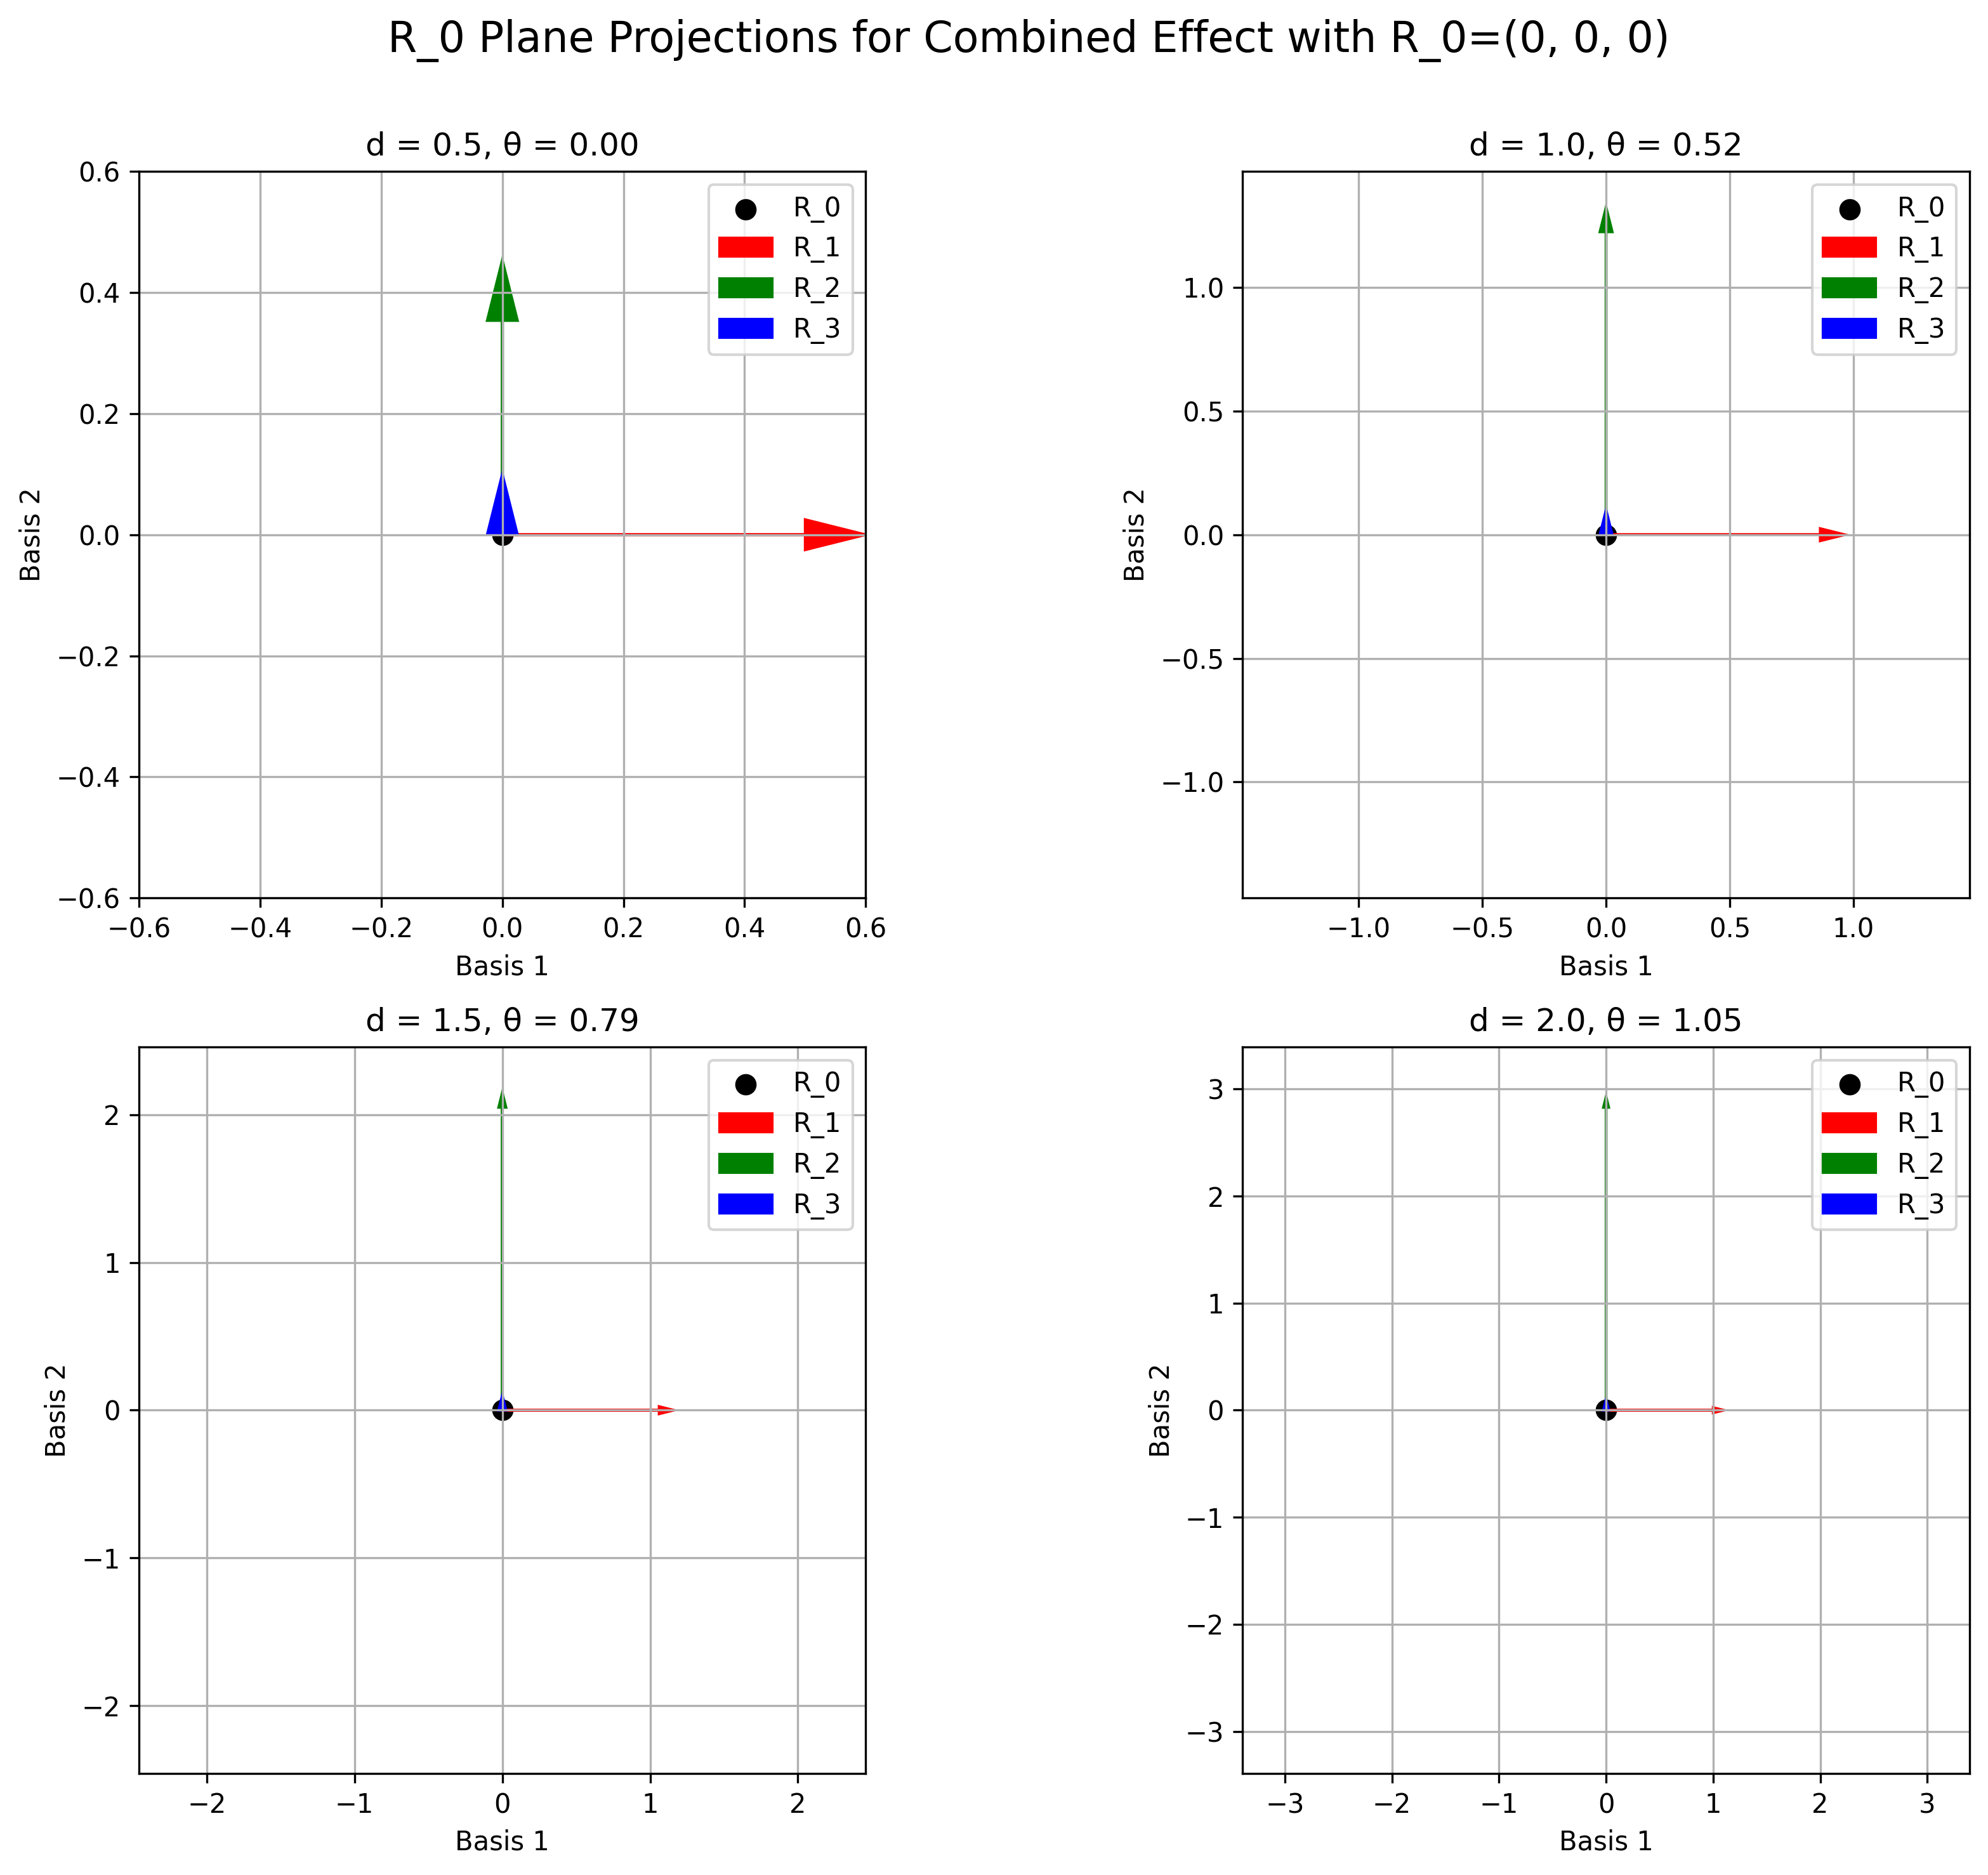
\includegraphics[width=0.9\textwidth]{figures/r0_projections_combined_effect_R0_0_0_0.png}
    \caption{$R_0$ plane projections for combined effect with origin at $(0,0,0)$}
    \label{fig:example_r0_projections_default}
\end{figure}

\begin{figure}[H]
    \centering
    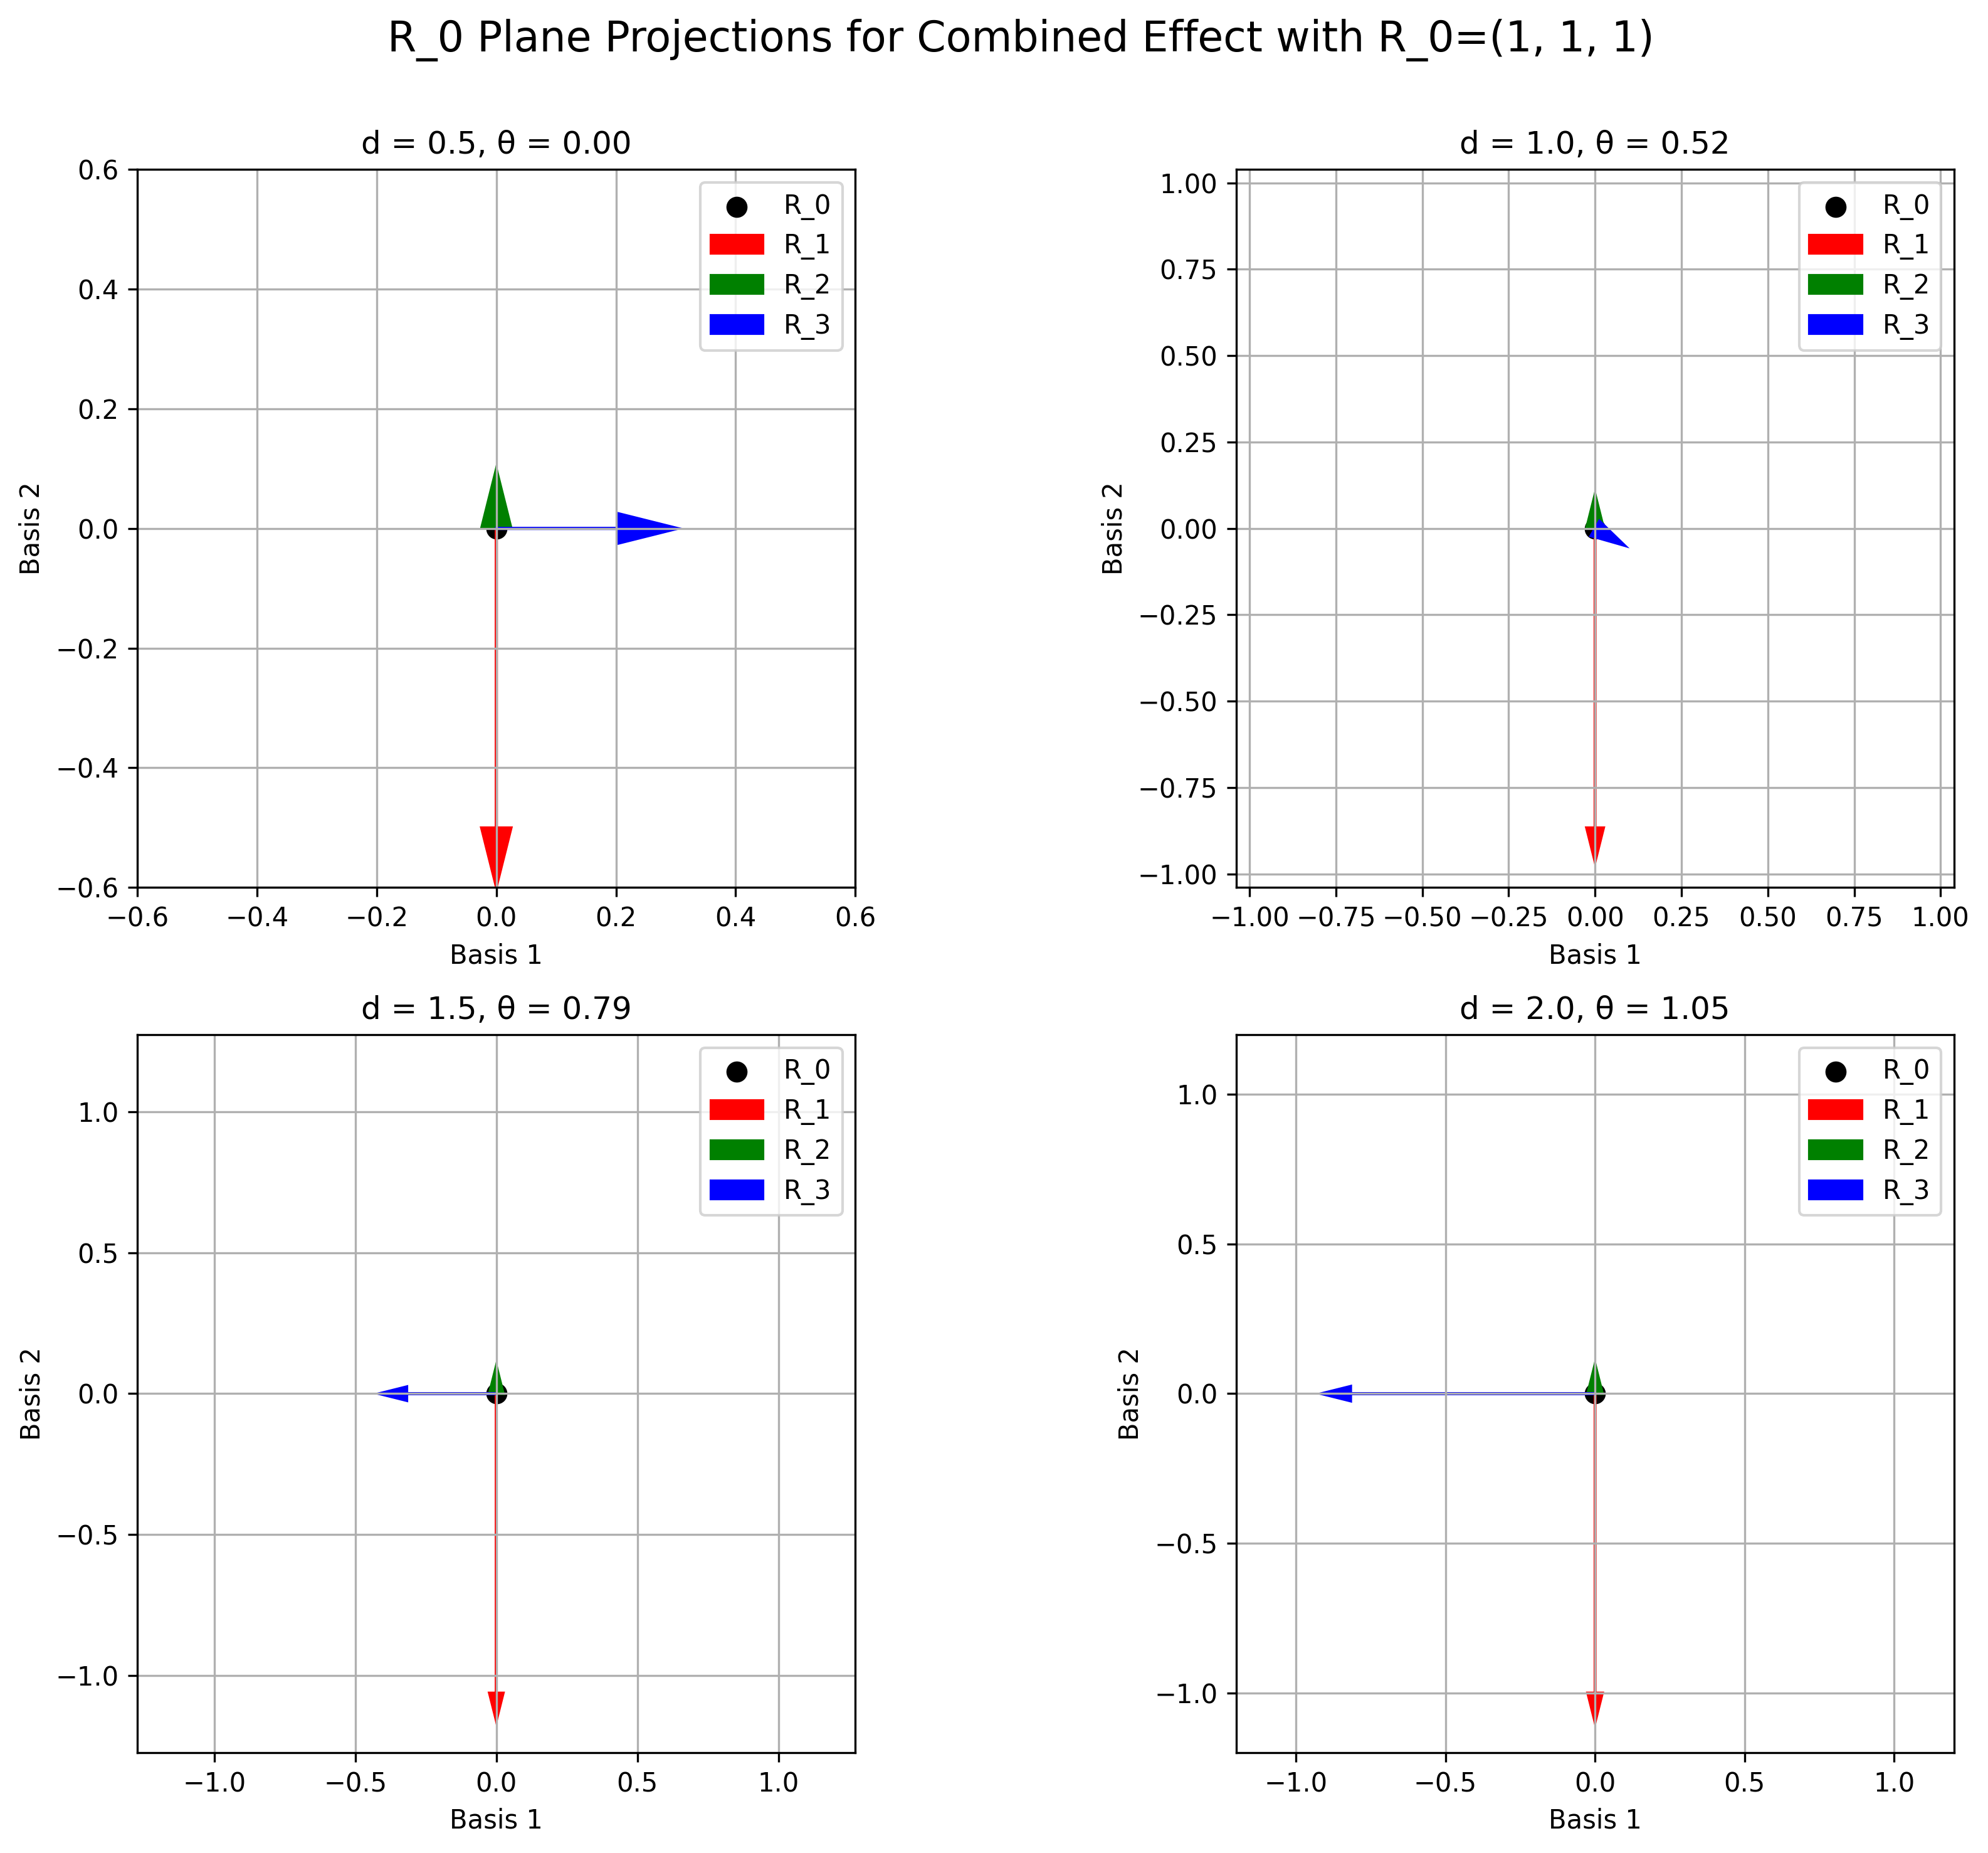
\includegraphics[width=0.9\textwidth]{figures/r0_projections_combined_effect_R0_1_1_1.png}
    \caption{$R_0$ plane projections for combined effect with origin at $(1,1,1)$}
    \label{fig:example_r0_projections_custom1}
\end{figure}

\begin{figure}[H]
    \centering
    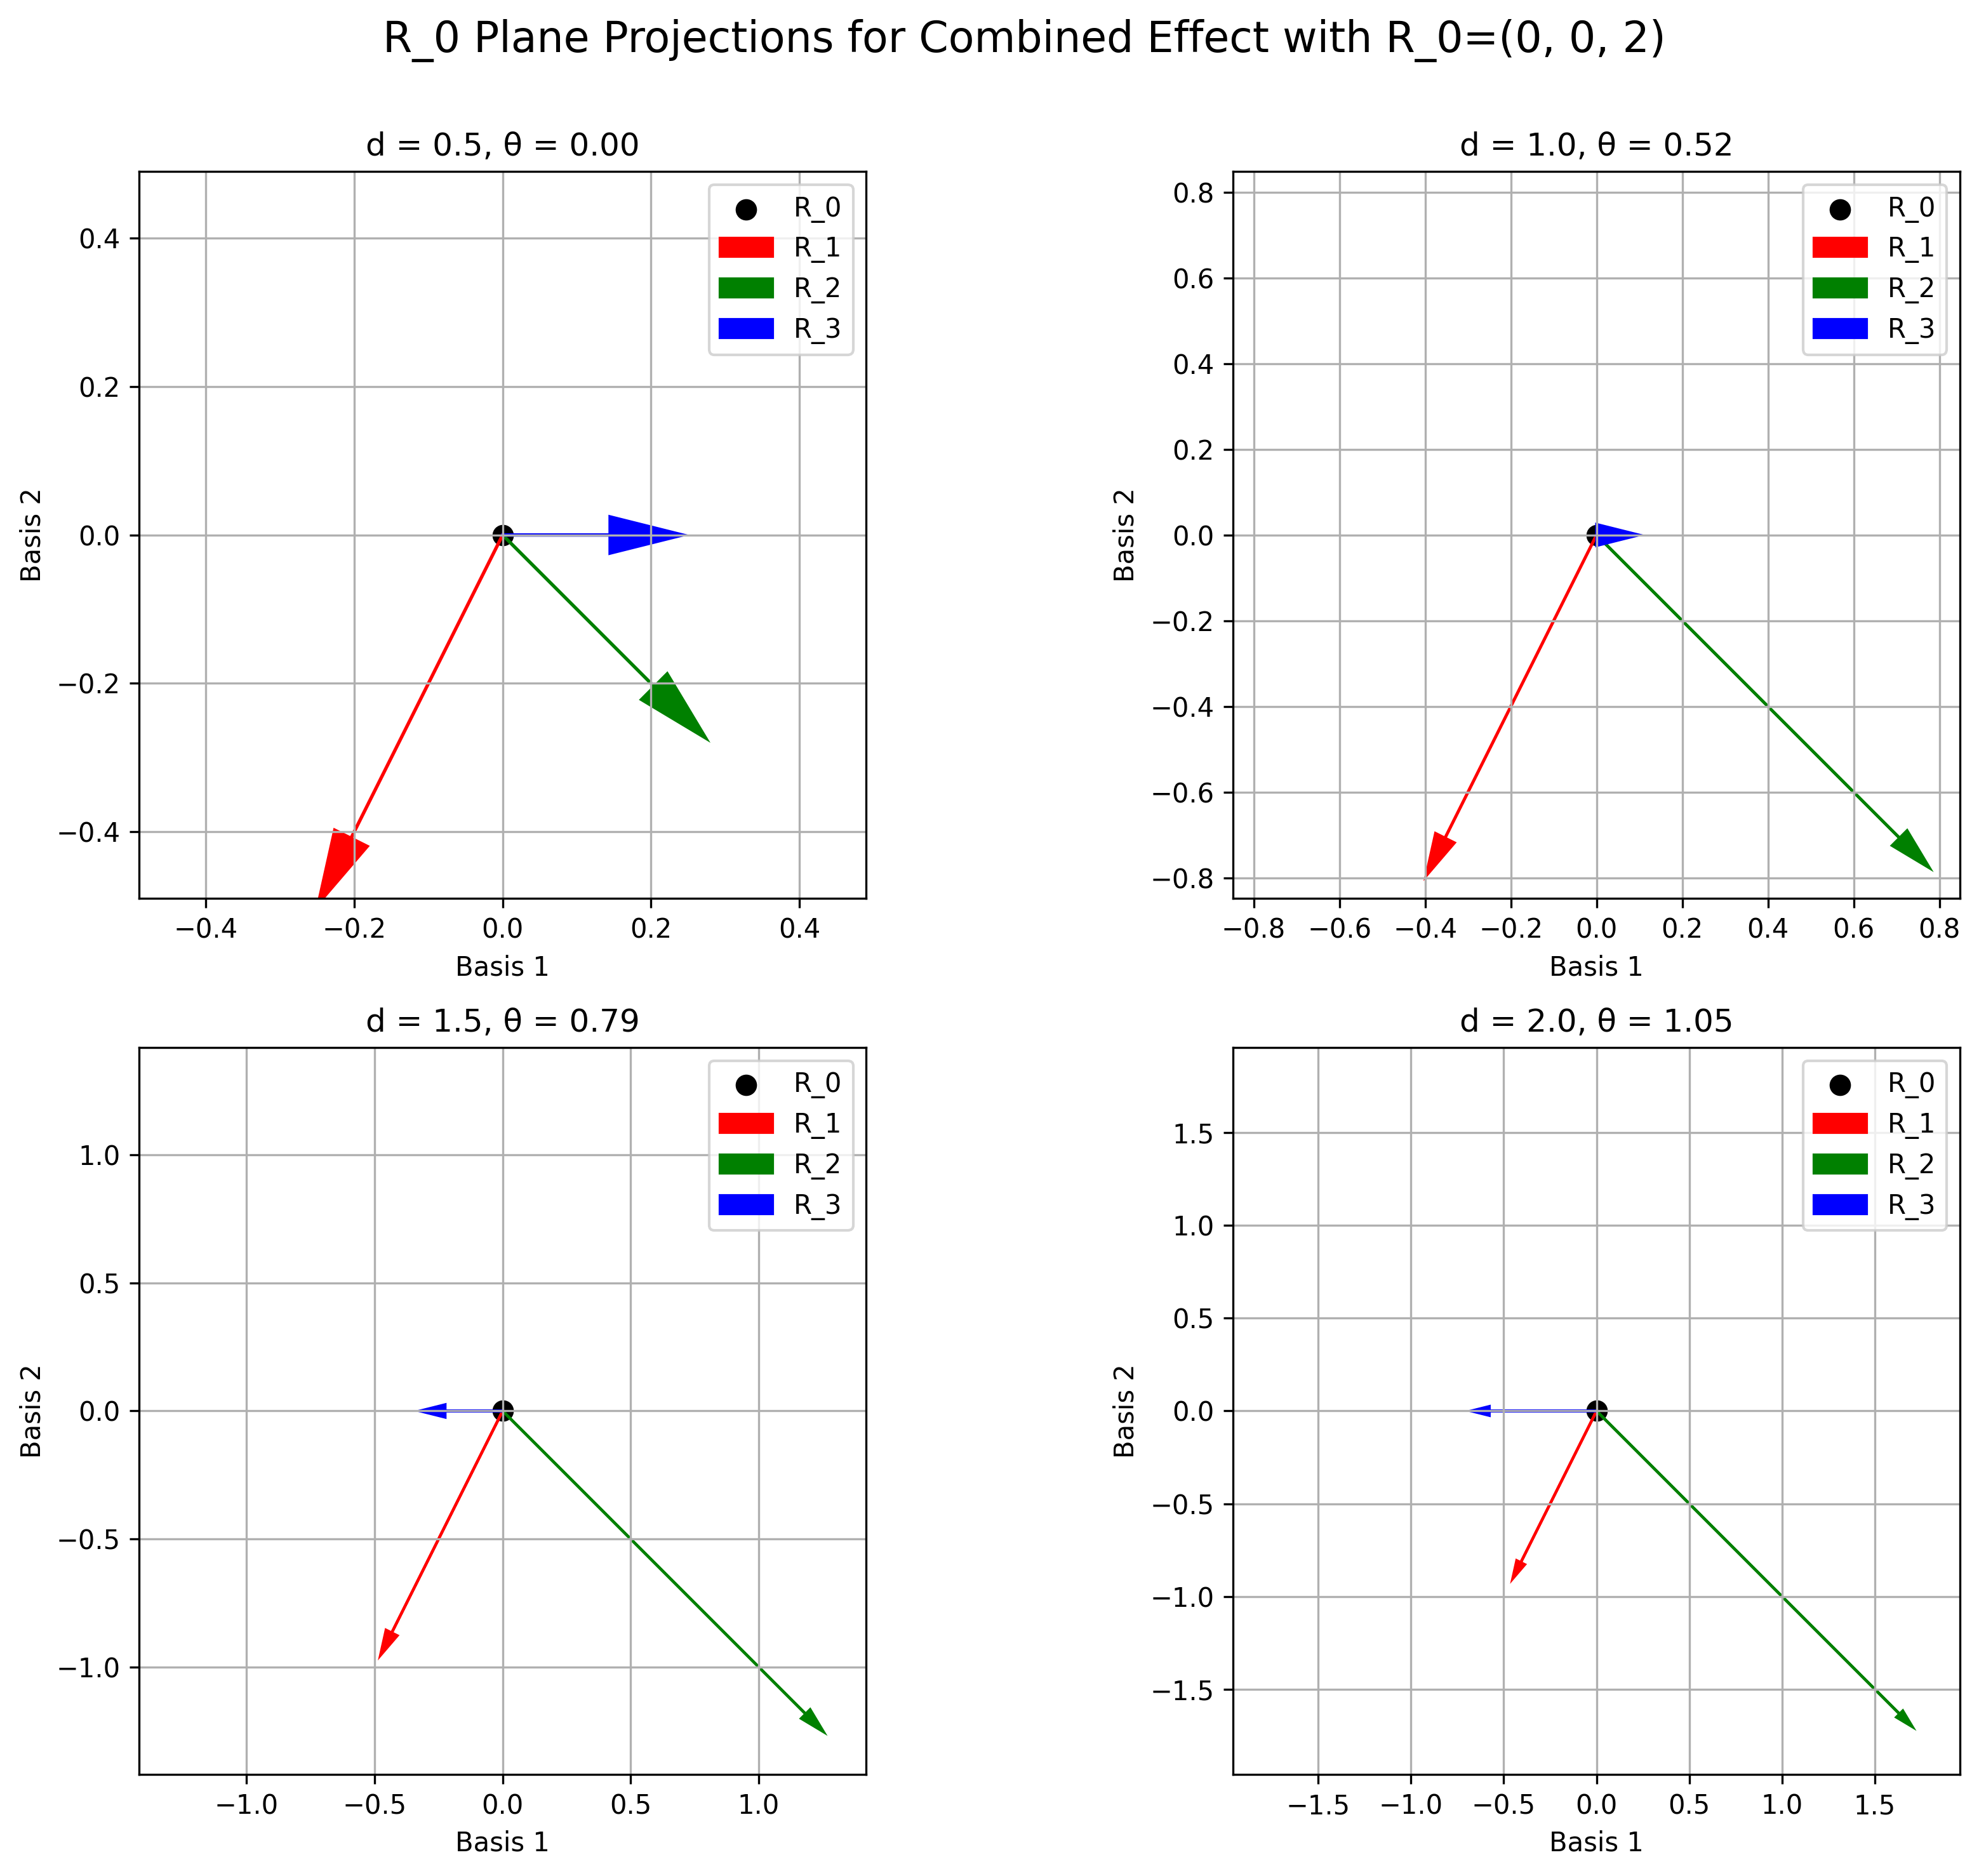
\includegraphics[width=0.9\textwidth]{figures/r0_projections_combined_effect_R0_0_0_2.png}
    \caption{$R_0$ plane projections for combined effect with origin at $(0,0,2)$}
    \label{fig:example_r0_projections_custom2}
\end{figure}

\subsubsection{Combined 3D and $R_0$ Plane Views}

The combined views show both the 3D vectors and their $R_0$ plane projections side by side, providing a comprehensive understanding of the vector relationships.

\begin{figure}[H]
    \centering
    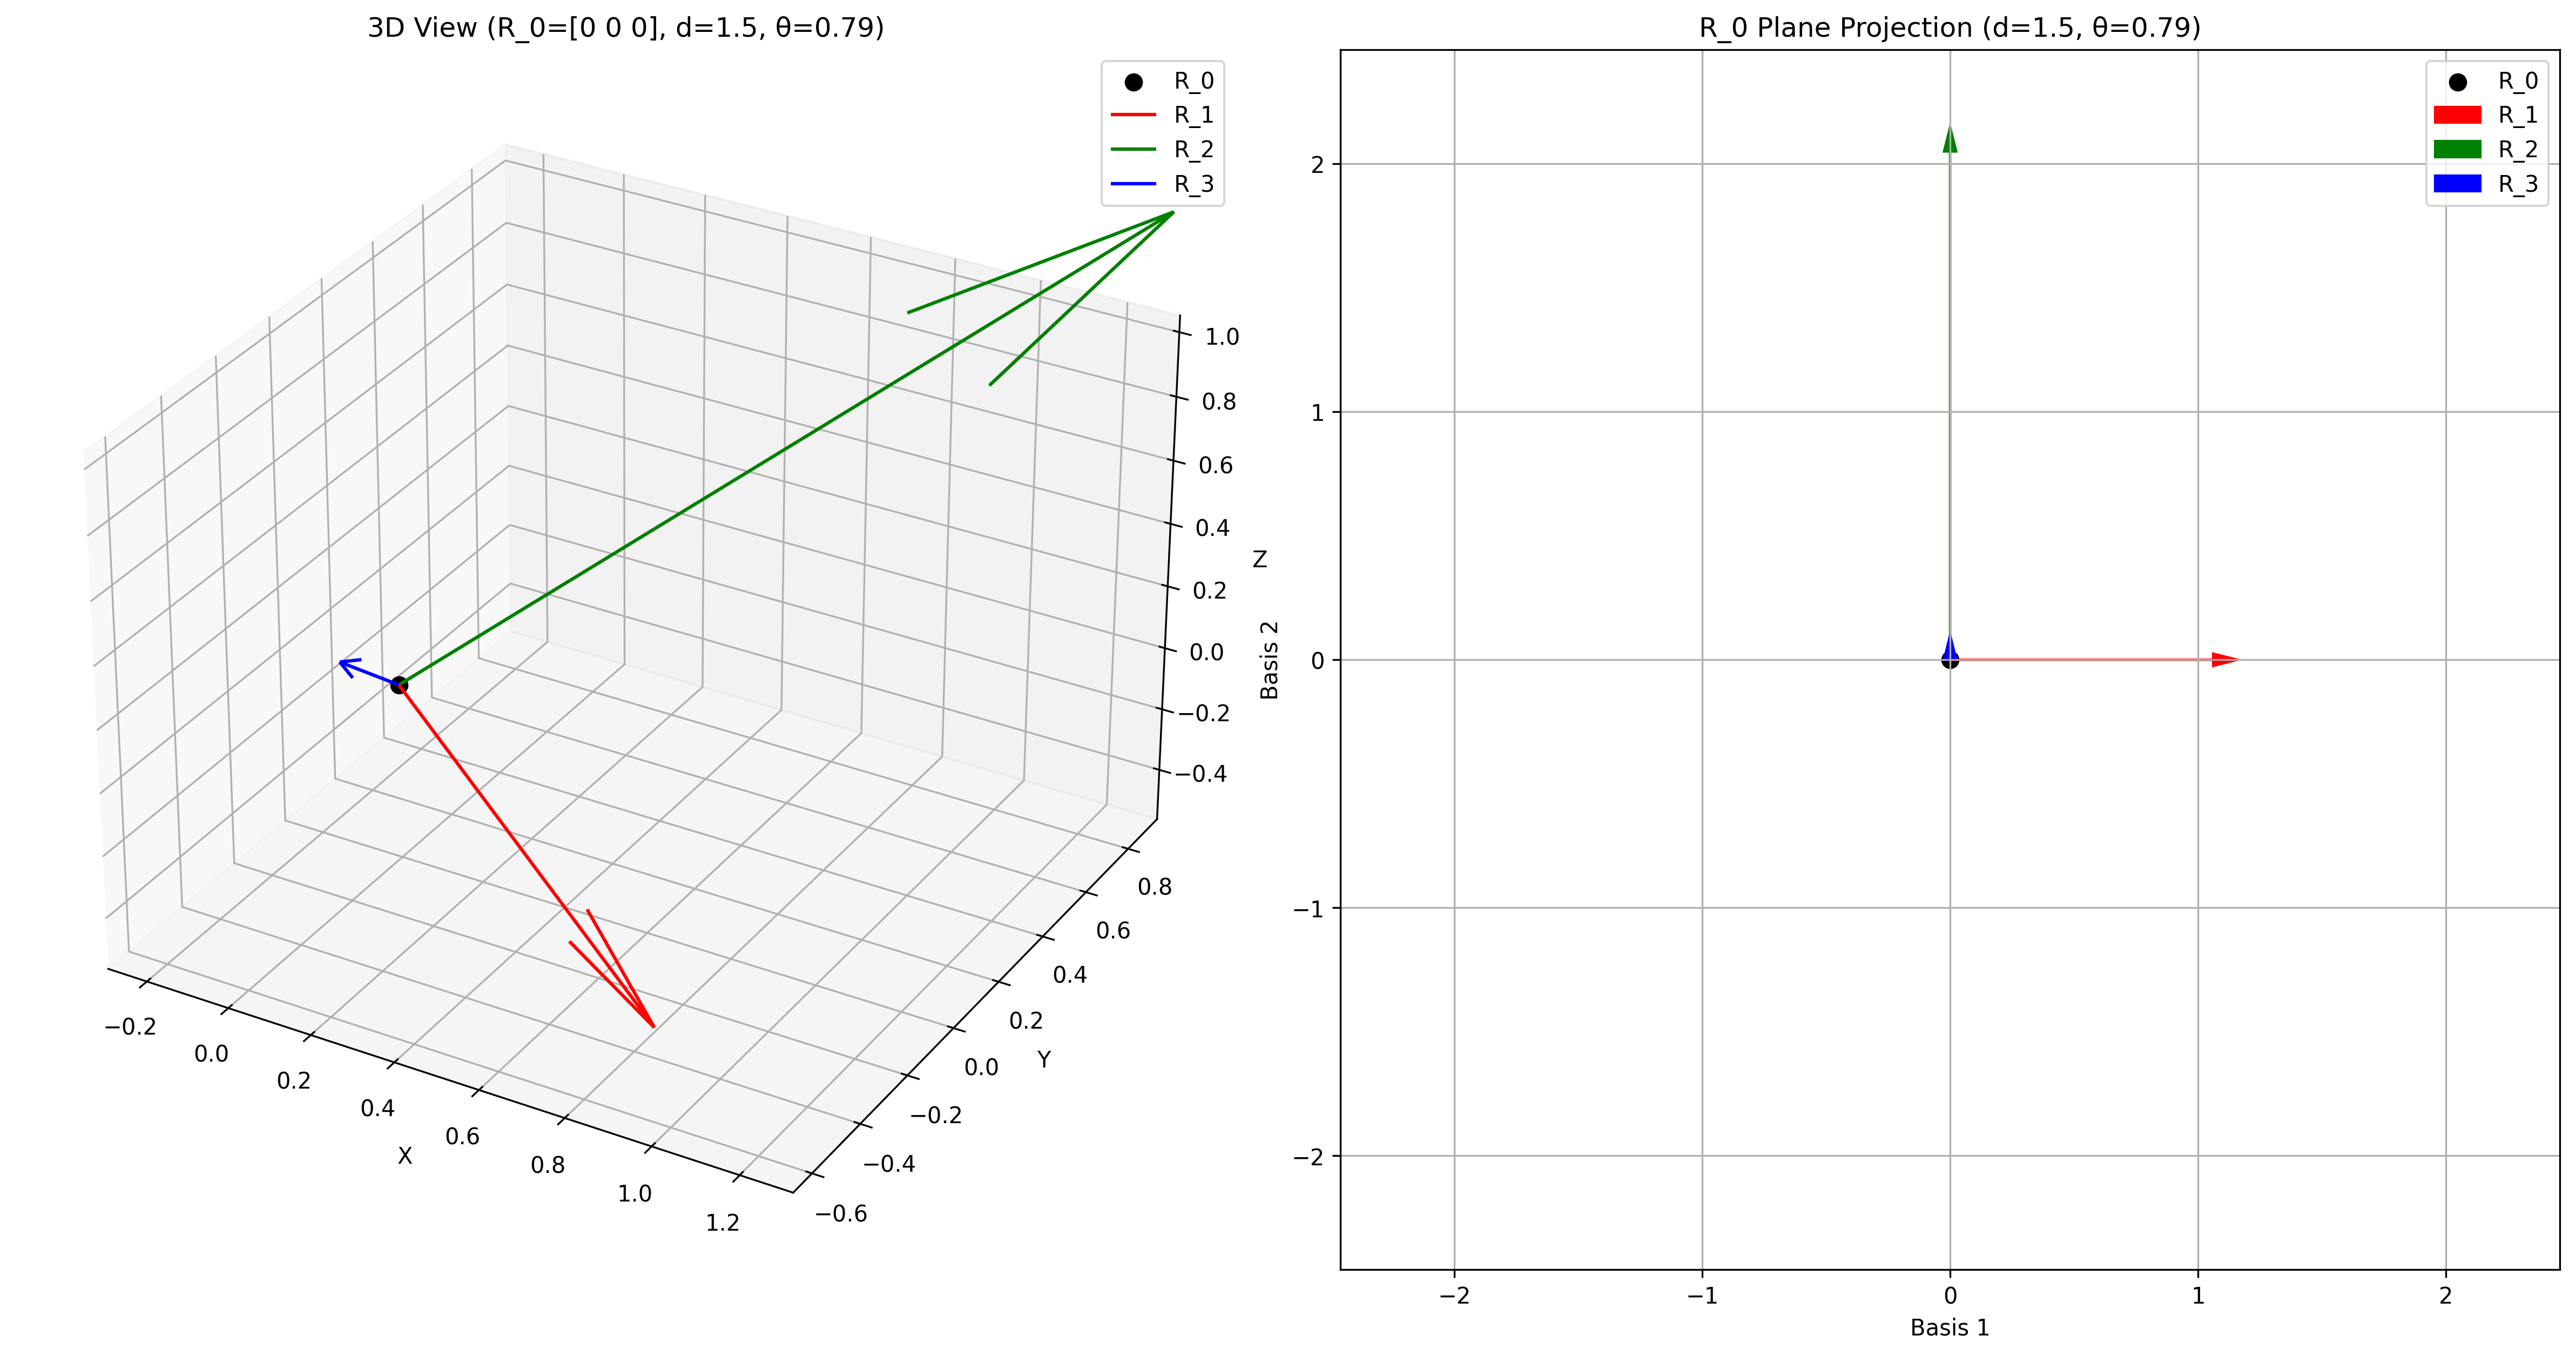
\includegraphics[width=0.9\textwidth]{figures/combined_view_R0_0_0_0_d_1p5_theta_0p79.png}
    \caption{Combined 3D and $R_0$ plane view with origin at $(0,0,0)$, $d=1.5$, $\theta=\pi/4$}
    \label{fig:example_combined_view_default}
\end{figure}

\begin{figure}[H]
    \centering
    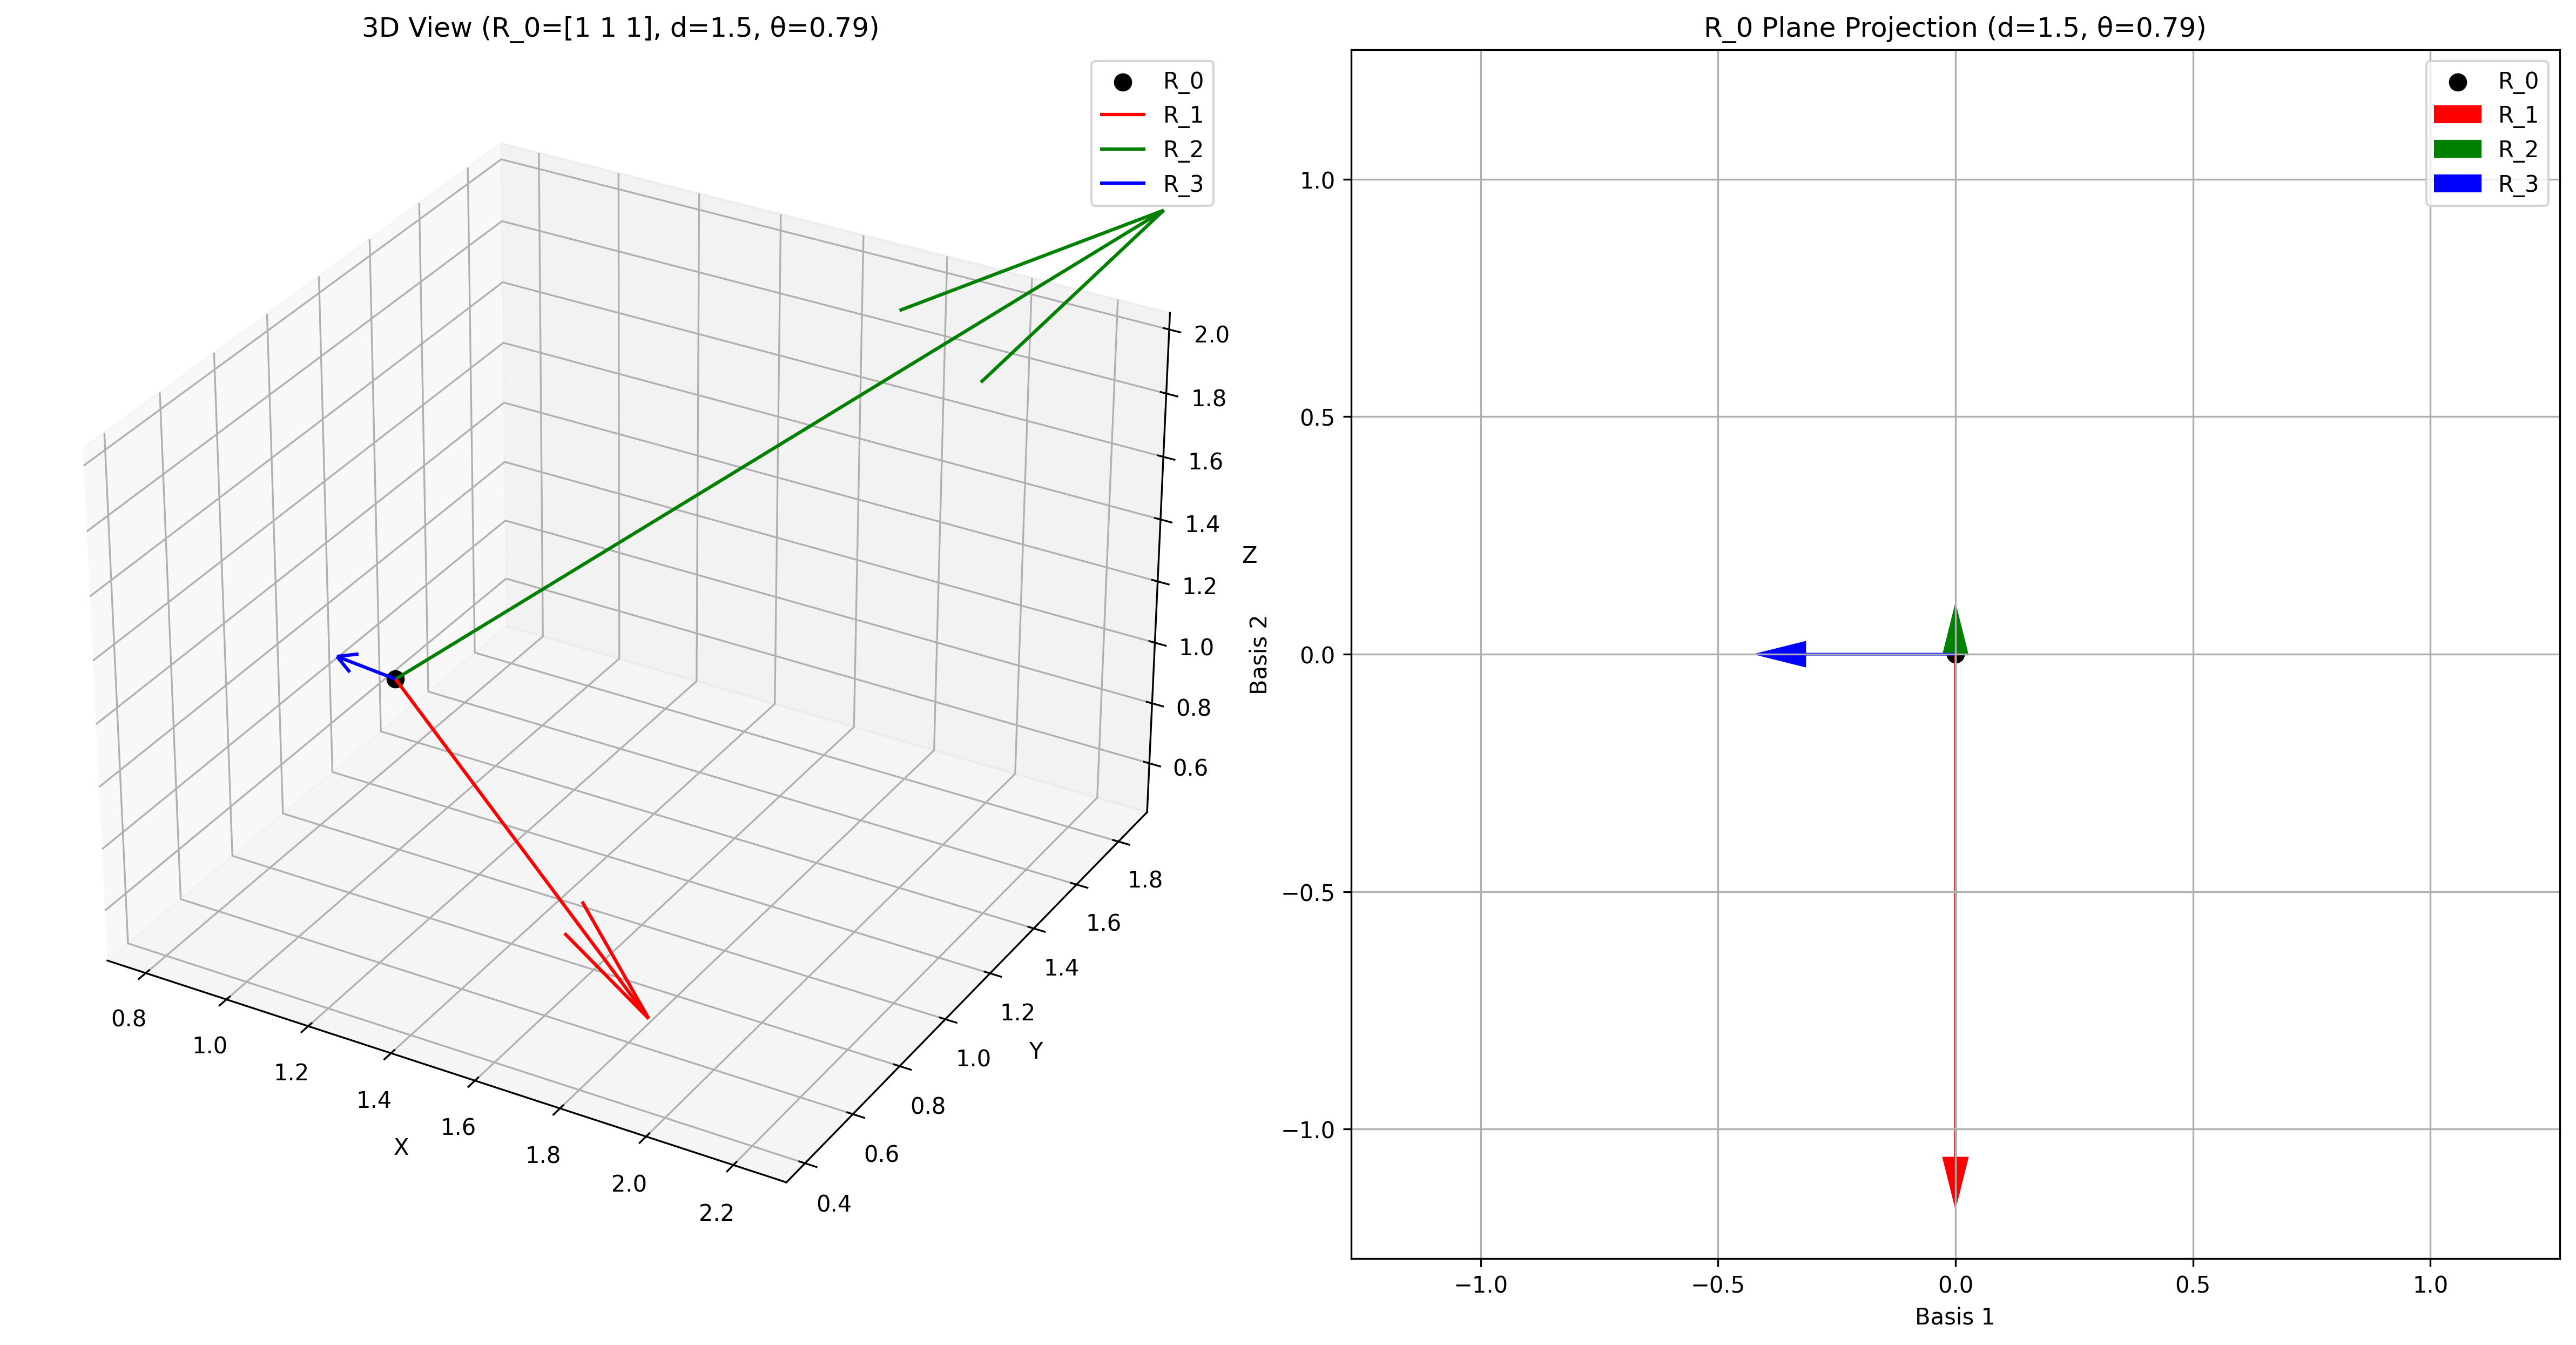
\includegraphics[width=0.9\textwidth]{figures/combined_view_R0_1_1_1_d_1p5_theta_0p79.png}
    \caption{Combined 3D and $R_0$ plane view with origin at $(1,1,1)$, $d=1.5$, $\theta=\pi/4$}
    \label{fig:example_combined_view_custom1}
\end{figure}

\begin{figure}[H]
    \centering
    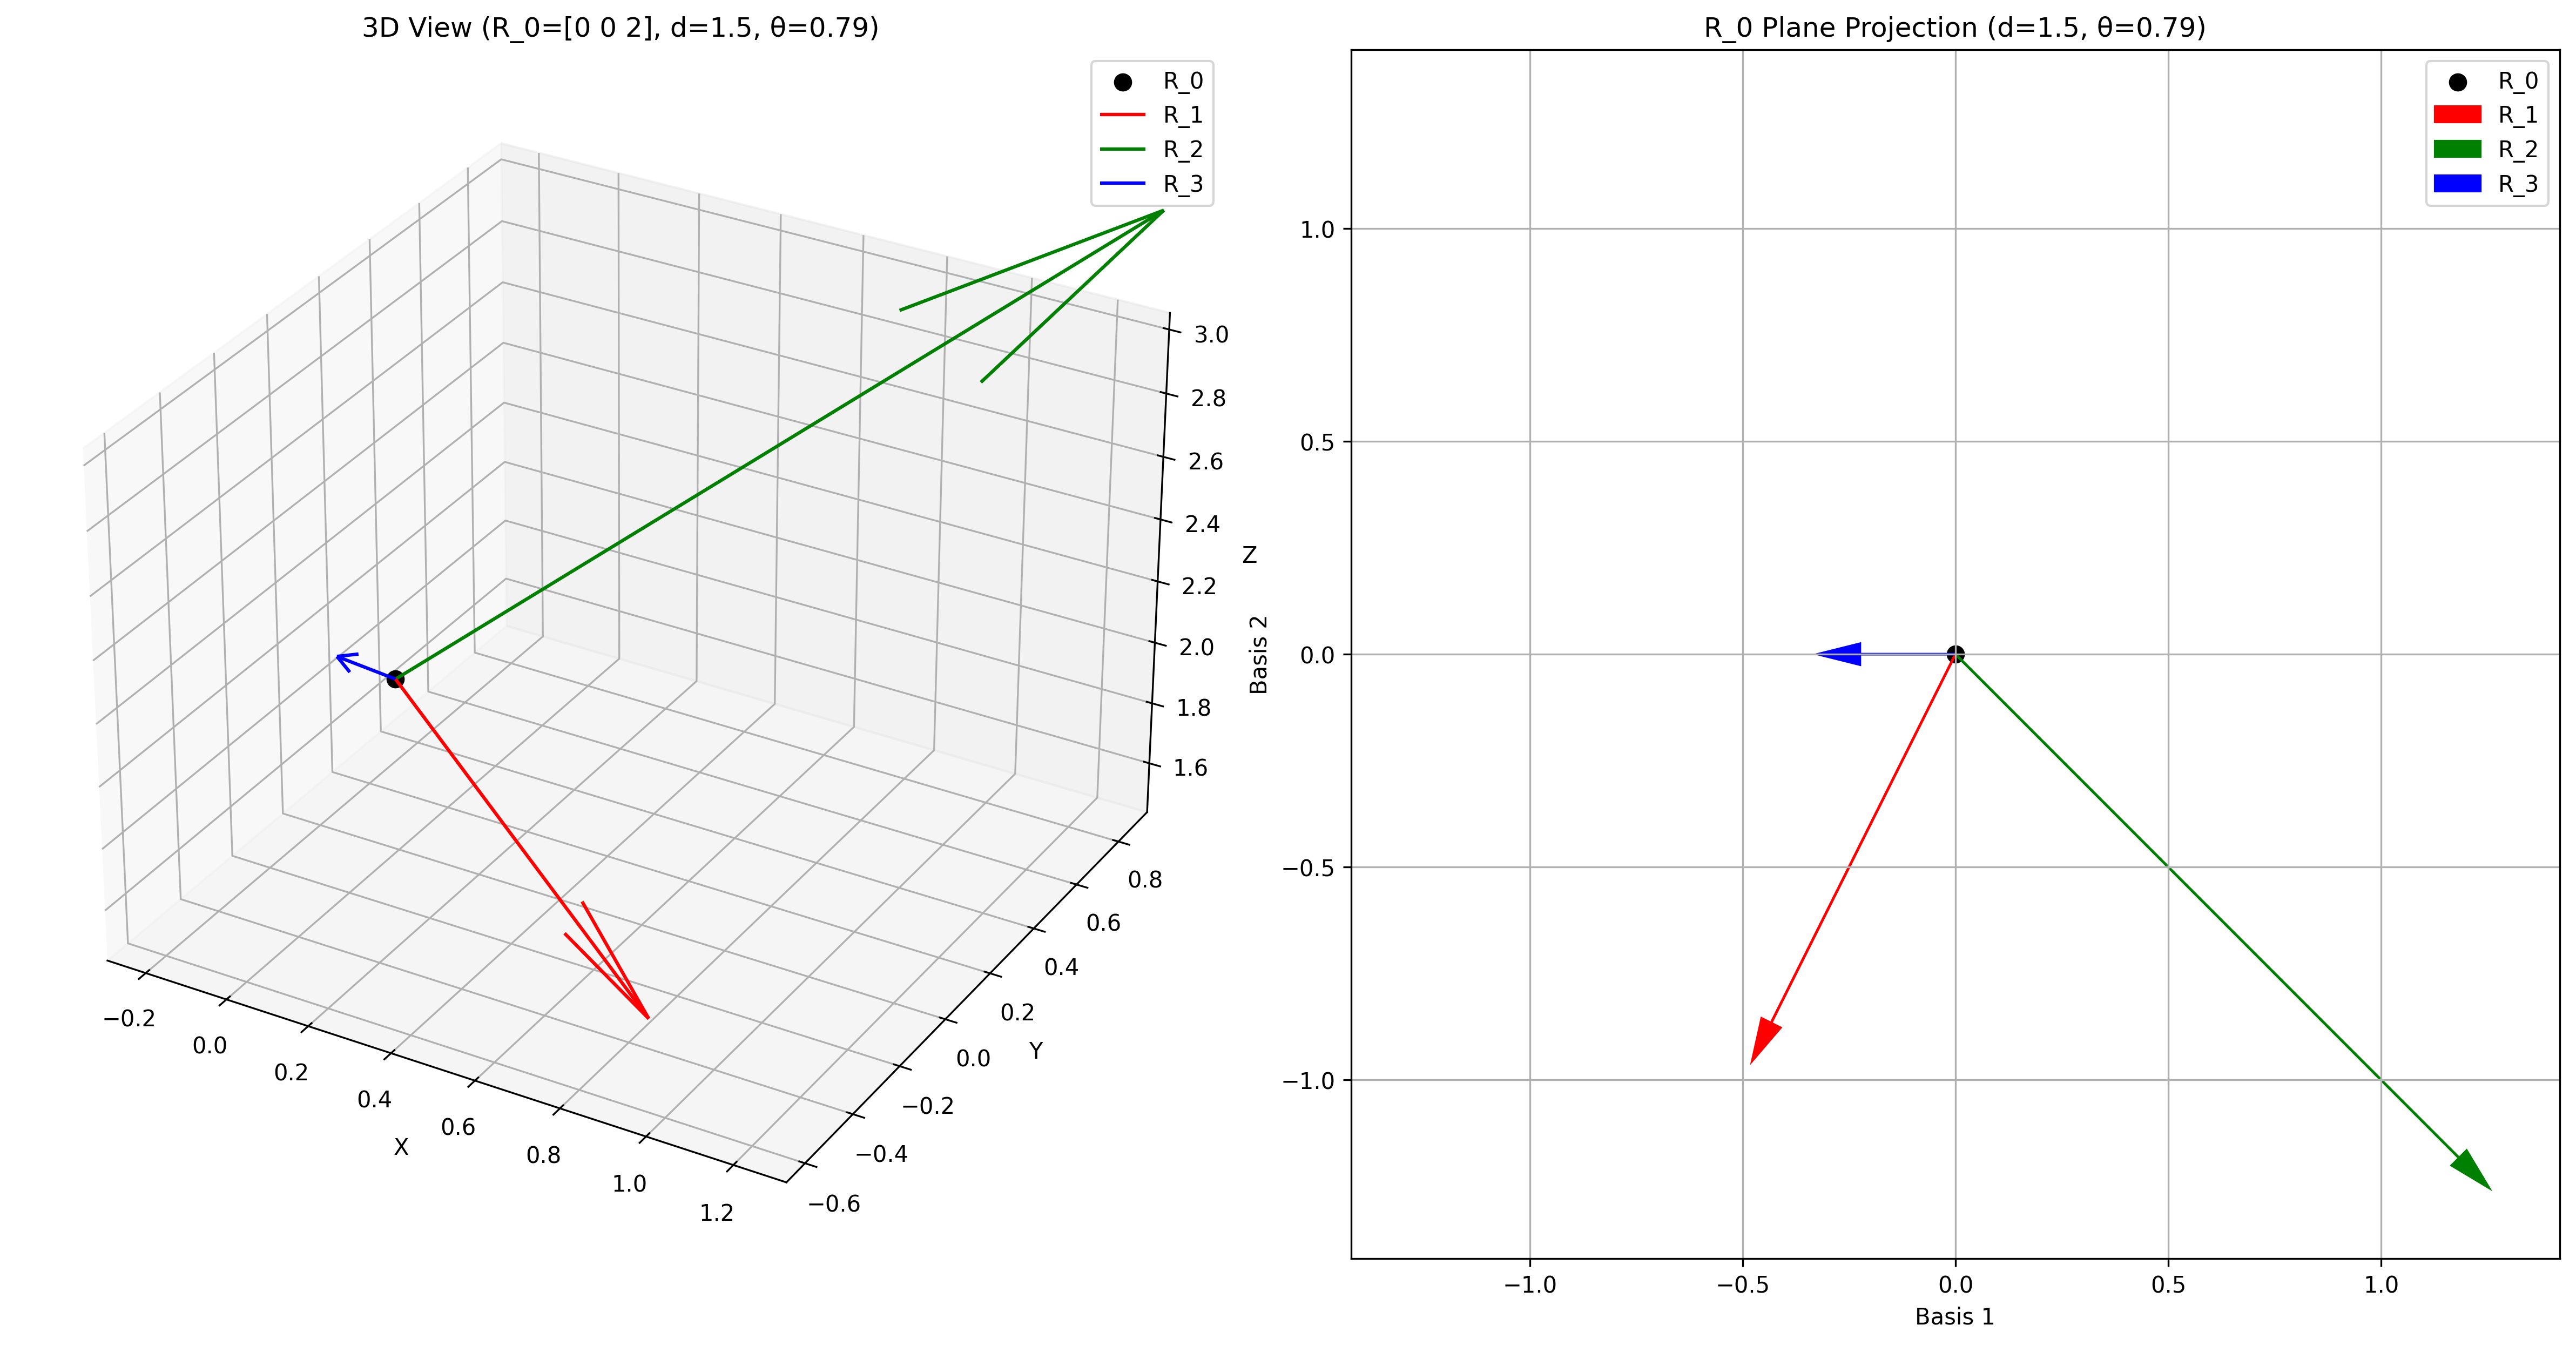
\includegraphics[width=0.9\textwidth]{figures/combined_view_R0_0_0_2_d_1p5_theta_0p79.png}
    \caption{Combined 3D and $R_0$ plane view with origin at $(0,0,2)$, $d=1.5$, $\theta=\pi/4$}
    \label{fig:example_combined_view_custom2}
\end{figure}

\textbf{Effect of Origin and Combined Parameters:} The origin parameter $\vec{R}_0$ shifts the entire vector system, preserving the orthogonality of the displacement vectors. Different origin points result in different positions of the vectors in space. The figures above demonstrate how different combinations of distance and angle parameters affect the vector visualization for each origin point. This illustrates the flexibility of the generalized orthogonal vectors implementation in creating various vector configurations.

\subsection{Summary of Results}

The example results demonstrate that the Generalized Orthogonal Vectors Generator and Visualizer successfully generates and visualizes orthogonal vectors for various configurations. The vectors are confirmed to be orthogonal by calculating their dot products, which are all zero (within numerical precision).

The visualizations show the vectors in both 3D and 2D projections, providing different perspectives on their spatial relationships. The effects of the distance parameter, angle parameter, and origin on the vector system are also demonstrated.

\section{Conclusion}

The Generalized Orthogonal Vectors Generator and Visualizer package provides a comprehensive solution for generating and visualizing orthogonal vectors in three-dimensional space. This document has described the mathematical formulation, implementation details, API reference, usage examples, visualization techniques, configuration system, command-line interface, and example results of the package.

\subsection{Summary of Features}

The package offers the following key features:

\begin{itemize}
    \item \textbf{Mathematical Rigor}: The package is based on a mathematically proven formulation for generating orthogonal vectors, ensuring the correctness of the results.
    
    \item \textbf{Modular Architecture}: The package is organized into separate modules for vector calculations, visualization, and configuration management, making it easy to maintain, extend, and reuse.
    
    \item \textbf{Configurability}: All aspects of vector generation and visualization can be configured through a unified configuration system, allowing for customization without modifying the code.
    
    \item \textbf{Command-line Interface}: The package provides a comprehensive command-line interface that allows users to generate and visualize orthogonal vectors without writing Python code.
    
    \item \textbf{Configuration File Support}: Configurations can be saved to and loaded from JSON files, making it easy to reuse configurations across different runs.
    
    \item \textbf{Multiple Visualization Options}: The package supports both 3D visualization and various 2D projections, providing different perspectives on the vectors.
    
    \item \textbf{Plot Saving}: Plots can be saved to files instead of being displayed interactively, allowing for the creation of visualizations for documentation or presentations.
    
    \item \textbf{Python Package}: The package can be used as a Python package, allowing for integration into other projects.
\end{itemize}

\subsection{Potential Applications}

The Generalized Orthogonal Vectors Generator and Visualizer package can be used in various applications, including:

\begin{itemize}
    \item \textbf{Educational Tools}: The package can be used as an educational tool for teaching concepts related to vectors, orthogonality, and three-dimensional geometry.
    
    \item \textbf{Scientific Visualization}: The package can be used for visualizing orthogonal vectors in scientific applications, such as physics simulations or computational geometry.
    
    \item \textbf{Computer Graphics}: The package can be used in computer graphics applications that require orthogonal coordinate systems, such as camera positioning or object orientation.
    
    \item \textbf{Robotics}: The package can be used in robotics applications that require orthogonal coordinate systems, such as robot arm positioning or sensor orientation.
\end{itemize}

\subsection{Future Work}

The Generalized Orthogonal Vectors Generator and Visualizer package can be extended in various ways, including:

\begin{itemize}
    \item \textbf{Additional Visualization Options}: The package could be extended to support additional visualization options, such as interactive 3D visualization or animation of vector rotation.
    
    \item \textbf{More Advanced Configuration Management}: The configuration management system could be extended to support more advanced features, such as configuration validation or configuration inheritance.
    
    \item \textbf{Integration with Other Packages}: The package could be integrated with other Python packages for scientific computing or visualization, such as SciPy or Plotly.
    
    \item \textbf{Web Interface}: The package could be extended to provide a web interface for generating and visualizing orthogonal vectors, making it accessible to users without Python knowledge.
    
    \item \textbf{Performance Optimization}: The package could be optimized for performance, especially for applications that require generating and visualizing a large number of vectors.
    
    \item \textbf{Unit Tests}: The package could be extended with comprehensive unit tests to ensure the correctness of the implementation.
    
    \item \textbf{Documentation Improvements}: The documentation could be improved with more examples, tutorials, and explanations of the mathematical concepts.
\end{itemize}

\subsection{Conclusion}

The Generalized Orthogonal Vectors Generator and Visualizer package provides a powerful and flexible tool for generating and visualizing orthogonal vectors in three-dimensional space. Its modular architecture, configurability, and comprehensive features make it suitable for a wide range of applications, from educational tools to scientific visualization. The package is designed to be easy to use, both as a command-line tool and as a Python package, making it accessible to users with different levels of programming experience.


\appendix
\section{Source Code}

This appendix contains the complete source code for the Generalized Orthogonal Vectors Generator and Visualizer package.

\subsection{main.py}

\begin{lstlisting}[language=Python]
#!/usr/bin/env python3
import numpy as np
import matplotlib.pyplot as plt
import argparse
import math
import os
import sys

from vector_utils import create_orthogonal_vectors, check_orthogonality
from visualization import plot_vectors_3d, plot_vectors_2d_projection, plot_all_projections
from config import VectorConfig, default_config

def parse_arguments():
    """
    Parse command line arguments
    
    Returns:
    argparse.Namespace: Parsed arguments
    """
    parser = argparse.ArgumentParser(description='Generate and visualize orthogonal vectors')
    
    # Vector parameters
    parser.add_argument('--origin', '-R', type=float, nargs=3, default=[0, 0, 0],
                        help='Origin vector R_0 (x y z)')
    parser.add_argument('--distance', '-d', type=float, default=1,
                        help='Distance parameter d')
    parser.add_argument('--angle', '-a', type=float, default=math.pi/4,
                        help='Angle parameter theta in radians')
    
    # Visualization parameters
    parser.add_argument('--no-r0-plane', action='store_false', dest='show_r0_plane',
                        help='Do not show the R_0 plane projection')
    parser.add_argument('--no-legend', action='store_false', dest='show_legend',
                        help='Do not show the legend')
    parser.add_argument('--no-grid', action='store_false', dest='show_grid',
                        help='Do not show the grid')
    
    # Output parameters
    parser.add_argument('--save-plots', action='store_true',
                        help='Save plots to files instead of displaying them')
    parser.add_argument('--output-dir', type=str, default='plots',
                        help='Directory to save plots to')
    parser.add_argument('--config', type=str,
                        help='Path to configuration file')
    parser.add_argument('--save-config', type=str,
                        help='Save configuration to file')
    
    return parser.parse_args()

def display_help():
    """
    Display detailed help information
    """
    help_text = """
    Orthogonal Vectors Generator and Visualizer
    =======================================
    
    This tool generates and visualizes three orthogonal vectors from a given origin point.
    
    Basic Usage:
    -----------
    python main.py                              # Use default parameters
    python main.py -R 1 1 1                    # Set origin to (1,1,1)
    python main.py -R 0 0 2 -d 1.5 -a 0.5236   # Custom origin, distance and angle
    python main.py --help                      # Show help
    
    Parameters:
    ----------
    -R, --origin X Y Z    : Set the origin vector R_0 coordinates (default: 0 0 0)
    -d, --distance VALUE  : Set the distance parameter (default: 1)
    -a, --angle VALUE     : Set the angle parameter in radians (default: \pi/4)
    
    Visualization Options:
    --------------------
    --no-r0-plane        : Do not show the R_0 plane projection
    --no-legend          : Do not show the legend
    --no-grid            : Do not show the grid
    
    Output Options:
    --------------
    --save-plots         : Save plots to files instead of displaying them
    --output-dir DIR     : Directory to save plots to (default: 'plots')
    
    Configuration:
    -------------
    --config FILE        : Load configuration from a JSON file
    --save-config FILE   : Save current configuration to a JSON file
    
    Examples:
    --------
    # Generate vectors with origin at (1,1,1), distance 2, and angle \pi/3
    python main.py -R 1 1 1 -d 2 -a 1.047
    
    # Save plots to a custom directory
    python main.py -R 0 0 2 --save-plots --output-dir my_plots
    
    # Load configuration from a file
    python main.py --config my_config.json
    """
    print(help_text)
    sys.exit(0)

def main():
    """
    Main function
    """
    # Check for detailed help command
    if len(sys.argv) > 1 and sys.argv[1] == 'help':
        display_help()
    
    # Parse command line arguments
    args = parse_arguments()
    
    # Load configuration
    if args.config:
        config = VectorConfig.load_from_file(args.config)
    else:
        # Create configuration from command line arguments
        config = VectorConfig(
            R_0=args.origin,
            d=args.distance,
            theta=args.angle,
            show_r0_plane=args.show_r0_plane,
            show_legend=args.show_legend,
            show_grid=args.show_grid
        )
    
    # Save configuration if requested
    if args.save_config:
        config.save_to_file(args.save_config)
    
    # Create the orthogonal vectors
    R_0 = config.R_0
    R_1, R_2, R_3 = create_orthogonal_vectors(R_0, config.d, config.theta)
    
    # Print vector information
    print("R_0:", R_0)
    print("R_1:", R_1)
    print("R_2:", R_2)
    print("R_3:", R_3)
    
    # Check orthogonality
    orthogonality = check_orthogonality(R_0, R_1, R_2, R_3)
    print("\nChecking orthogonality (dot products should be close to zero):")
    for key, value in orthogonality.items():
        print(f"{key}: {value}")
    
    # Plot the vectors
    plots = plot_all_projections(
        R_0, R_1, R_2, R_3,
        show_r0_plane=config.show_r0_plane,
        figsize_3d=config.figsize_3d,
        figsize_2d=config.figsize_2d
    )
    
    # Save or show the plots
    if args.save_plots:
        # Create output directory if it doesn't exist
        os.makedirs(args.output_dir, exist_ok=True)
        
        # Save each plot
        for name, (fig, _) in plots.items():
            filename = os.path.join(args.output_dir, f"{name}.png")
            fig.savefig(filename)
            print(f"Saved plot to {filename}")
    else:
        # Show the plots
        plt.show()

if __name__ == "__main__":
    main()
\end{lstlisting}

\subsection{vector\_utils.py}

\begin{lstlisting}[language=Python]
#!/usr/bin/env python3
import numpy as np

def create_orthogonal_vectors(R_0=(0, 0, 0), d=1, theta=0):
    """
    Create 3 orthogonal R vectors for R_0
    
    Parameters:
    R_0 (tuple or numpy.ndarray): The origin vector, default is (0, 0, 0)
    d (float): The distance parameter, default is 1
    theta (float): The angle parameter in radians, default is 0
    
    Returns:
    tuple: Three orthogonal vectors R_1, R_2, R_3
    """
    # Convert R_0 to numpy array for vector operations
    R_0 = np.array(R_0)
    
    # Calculate R_1, R_2, R_3 according to the given formulas
    # R_1 = R_0 + d * (cos(theta))*sqrt(2/3)
    R_1 = R_0 + d * np.cos(theta) * np.sqrt(2/3) * np.array([1, -1/2, -1/2])
    
    # R_2 = R_0 + d * (cos(theta)/sqrt(3) + sin(theta))/sqrt(2)
    R_2 = R_0 + d * (np.cos(theta)/np.sqrt(3) + np.sin(theta))/np.sqrt(2) * np.array([1, 1, 1])
    
    # R_3 = R_0 + d * (sin(theta) - cos(theta)/sqrt(3))/sqrt(2)
    R_3 = R_0 + d * (np.sin(theta) - np.cos(theta)/np.sqrt(3))/np.sqrt(2) * np.array([0, -1/2, 1/2]) * np.sqrt(2)
    
    return R_1, R_2, R_3

def check_orthogonality(R_0, R_1, R_2, R_3):
    """
    Check if the vectors R_1, R_2, R_3 are orthogonal with respect to R_0
    
    Parameters:
    R_0, R_1, R_2, R_3 (numpy.ndarray): The vectors to check
    
    Returns:
    dict: Dictionary containing the dot products between pairs of vectors
    """
    dot_1_2 = np.dot(R_1 - R_0, R_2 - R_0)
    dot_1_3 = np.dot(R_1 - R_0, R_3 - R_0)
    dot_2_3 = np.dot(R_2 - R_0, R_3 - R_0)
    
    return {
        "R_1 $\cdot$ R_2": dot_1_2,
        "R_1 $\cdot$ R_3": dot_1_3,
        "R_2 $\cdot$ R_3": dot_2_3
    }
\end{lstlisting}

\subsection{config.py}

\begin{lstlisting}[language=Python]
#!/usr/bin/env python3
import numpy as np
import math
import json
import os

class VectorConfig:
    """
    Configuration class for orthogonal vector generation and visualization
    """
    def __init__(self, 
                 R_0=(0, 0, 0), 
                 d=1, 
                 theta=math.pi/4,
                 show_r0_plane=True,
                 figsize_3d=(10, 8),
                 figsize_2d=(8, 8),
                 show_legend=True,
                 show_grid=True):
        """
        Initialize the configuration
        
        Parameters:
        R_0 (tuple or list): The origin vector
        d (float): The distance parameter
        theta (float): The angle parameter in radians
        show_r0_plane (bool): Whether to show the R_0 plane projection
        figsize_3d (tuple): Figure size for 3D plot
        figsize_2d (tuple): Figure size for 2D plots
        show_legend (bool): Whether to show the legend
        show_grid (bool): Whether to show the grid
        """
        self.R_0 = np.array(R_0)
        self.d = d
        self.theta = theta
        self.show_r0_plane = show_r0_plane
        self.figsize_3d = figsize_3d
        self.figsize_2d = figsize_2d
        self.show_legend = show_legend
        self.show_grid = show_grid
    
    def to_dict(self):
        """
        Convert the configuration to a dictionary
        
        Returns:
        dict: Dictionary representation of the configuration
        """
        return {
            'R_0': self.R_0.tolist(),
            'd': self.d,
            'theta': self.theta,
            'show_r0_plane': self.show_r0_plane,
            'figsize_3d': self.figsize_3d,
            'figsize_2d': self.figsize_2d,
            'show_legend': self.show_legend,
            'show_grid': self.show_grid
        }
    
    @classmethod
    def from_dict(cls, config_dict):
        """
        Create a configuration from a dictionary
        
        Parameters:
        config_dict (dict): Dictionary containing configuration parameters
        
        Returns:
        VectorConfig: Configuration object
        """
        return cls(
            R_0=config_dict.get('R_0', (0, 0, 0)),
            d=config_dict.get('d', 1),
            theta=config_dict.get('theta', math.pi/4),
            show_r0_plane=config_dict.get('show_r0_plane', True),
            figsize_3d=config_dict.get('figsize_3d', (10, 8)),
            figsize_2d=config_dict.get('figsize_2d', (8, 8)),
            show_legend=config_dict.get('show_legend', True),
            show_grid=config_dict.get('show_grid', True)
        )
    
    def save_to_file(self, filename):
        """
        Save the configuration to a JSON file
        
        Parameters:
        filename (str): Path to the output file
        """
        with open(filename, 'w') as f:
            json.dump(self.to_dict(), f, indent=4)
    
    @classmethod
    def load_from_file(cls, filename):
        """
        Load a configuration from a JSON file
        
        Parameters:
        filename (str): Path to the input file
        
        Returns:
        VectorConfig: Configuration object
        """
        if not os.path.exists(filename):
            print(f"Warning: Config file {filename} not found. Using default configuration.")
            return cls()
        
        with open(filename, 'r') as f:
            config_dict = json.load(f)
        
        return cls.from_dict(config_dict)

# Default configuration
default_config = VectorConfig()
\end{lstlisting}

\subsection{visualization.py}

\begin{lstlisting}[language=Python]
#!/usr/bin/env python3
import numpy as np
import matplotlib.pyplot as plt
from mpl_toolkits.mplot3d import Axes3D

def plot_vectors_3d(R_0, R_1, R_2, R_3, figsize=(10, 8), show_legend=True):
    """
    Plot the vectors in 3D
    
    Parameters:
    R_0 (numpy.ndarray): The origin vector
    R_1, R_2, R_3 (numpy.ndarray): The three orthogonal vectors
    figsize (tuple): Figure size (width, height) in inches
    show_legend (bool): Whether to show the legend
    
    Returns:
    tuple: (fig, ax) matplotlib figure and axis objects
    """
    fig = plt.figure(figsize=figsize)
    ax = fig.add_subplot(111, projection='3d')
    
    # Plot the origin
    ax.scatter(R_0[0], R_0[1], R_0[2], color='black', s=100, label='R_0')
    
    # Plot the vectors as arrows from the origin
    vectors = [R_1, R_2, R_3]
    colors = ['r', 'g', 'b']
    labels = ['R_1', 'R_2', 'R_3']
    
    for i, (vector, color, label) in enumerate(zip(vectors, colors, labels)):
        ax.quiver(R_0[0], R_0[1], R_0[2], 
                 vector[0]-R_0[0], vector[1]-R_0[1], vector[2]-R_0[2], 
                 color=color, label=label, arrow_length_ratio=0.1)
    
    # Set labels and title
    ax.set_xlabel('X')
    ax.set_ylabel('Y')
    ax.set_zlabel('Z')
    ax.set_title('3D Plot of Orthogonal Vectors')
    
    # Set equal aspect ratio
    max_range = np.array([
        np.max([R_0[0], R_1[0], R_2[0], R_3[0]]) - np.min([R_0[0], R_1[0], R_2[0], R_3[0]]),
        np.max([R_0[1], R_1[1], R_2[1], R_3[1]]) - np.min([R_0[1], R_1[1], R_2[1], R_3[1]]),
        np.max([R_0[2], R_1[2], R_2[2], R_3[2]]) - np.min([R_0[2], R_1[2], R_2[2], R_3[2]])
    ]).max() / 2.0
    
    mid_x = (np.max([R_0[0], R_1[0], R_2[0], R_3[0]]) + np.min([R_0[0], R_1[0], R_2[0], R_3[0]])) / 2
    mid_y = (np.max([R_0[1], R_1[1], R_2[1], R_3[1]]) + np.min([R_0[1], R_1[1], R_2[1], R_3[1]])) / 2
    mid_z = (np.max([R_0[2], R_1[2], R_2[2], R_3[2]]) + np.min([R_0[2], R_1[2], R_2[2], R_3[2]])) / 2
    
    ax.set_xlim(mid_x - max_range, mid_x + max_range)
    ax.set_ylim(mid_y - max_range, mid_y + max_range)
    ax.set_zlim(mid_z - max_range, mid_z + max_range)
    
    if show_legend:
        ax.legend()
    
    return fig, ax

# Note: This is a partial listing. The full visualization.py file contains additional functions
# such as plot_vectors_2d_projection and plot_all_projections that are omitted here for brevity.
\end{lstlisting}

\subsection{\_\_init\_\_.py}

\begin{lstlisting}[language=Python]
# Generalized Orthogonal Vectors Generator and Visualizer
# This package provides tools for generating and visualizing orthogonal vectors

from .vector_utils import create_orthogonal_vectors, check_orthogonality
from .visualization import plot_vectors_3d, plot_vectors_2d_projection, plot_all_projections
from .config import VectorConfig, default_config

__all__ = [
    'create_orthogonal_vectors',
    'check_orthogonality',
    'plot_vectors_3d',
    'plot_vectors_2d_projection',
    'plot_all_projections',
    'VectorConfig',
    'default_config'
]

__version__ = '1.0.0'
\end{lstlisting}


\end{document}
